\documentclass[sfheadings,a4paper,10pt,floats,floatfix]{article}
\usepackage[margin=0.7in]{geometry}
\usepackage{graphicx}
\usepackage{verbatim}
\usepackage{bookmark}
\usepackage{float,url}% to fix the figure at the exact position
% \restylefloat{figure}
%\usepackage{hyperref}
% \usepackage{latin1}%{inputenc}
\usepackage{mathrsfs}
\usepackage{amssymb}
\usepackage{amsmath}
\usepackage{bm}
\usepackage{color}
\usepackage[table]{xcolor}% http://ctan.org/pkg/xcolor
\usepackage{multirow}
% \usepackage{caption}
\usepackage{subfig}%
% \usepackage{subcaption}
\newcommand{\bra}[1]{\left(#1\right)}
\newcommand{\loge}[1]{\text{#1}}
\newcommand{\bras}[1]{\left[#1\right]}
\newcommand{\brac}[1]{\left\{#1\right\}}
\newcommand{\bral}[1]{\left|#1\right|}
\newcommand{\ber}{\begin{eqnarray}}
\newcommand{\eer}{\end{eqnarray}}
\newcommand{\ETAL}{{\it et al.}}  
\newcommand{\be}{\begin{equation}}
\newcommand{\ee}{\end{equation}}
\newcommand{\ba}{\begin{eqnarray}}
\newcommand{\ea}{\end{eqnarray}}
\newcommand{\hld}{\hspace{0.25cm}\cdots}
\newcommand{\fns}{\footnotesize}
\newcommand{\fnsc}{\scriptsize}
\newcommand{\mbs}[1]{\mbox{\small #1}}
\newcommand{\la}{\langle}
\newcommand{\ra}{\rangle}

 

\voffset .5in
\title{SKA1-Mid Scale-Dependent Sensitivity}
\author{O. M. Smirnov$^{1,2}$, S. Makhathini$^{1,2}$, M. Jarvis$^{3,4}$ and F. B. Abdalla$^5$ \\{\footnotesize \it $^1$Rhodes
University, Artillery Road P O Box 94, Grahamstown 6140, South Africa} \\{ \footnotesize \it $^2$SKA South Africa, 3rd Floor,
Park Road, Pinelands, 7405, South Africa} \\{\footnotesize \it $^3$ University of the Western Cape, ZA-7535 Cape Town, South
Africa}\\ {\footnotesize \it $^4$University of Oxford, Oxford OX1 3RH, England} \\ {\footnotesize \it $^5$Department of Physics
and Astronomy, University College London,Gower Place, London WC1E 6BT, United Kingdom}}
% \date{}
\begin{document}
\maketitle
\begin{abstract}
In this report we study the scale dependent sensitivity of the SKA1-Mid baseline design. We also propose changes to the baseline
design that enhance the sensitivity at smaller angular scales (say 0.4-1 arcsec at 650MHz) without compromising the performance at
larger scales. The changes we propose are guided by the SKA1-Mid level-zero science requirements \cite{srd}, which suggest that
baselines larger than 100km are not necessary to achieve the SKA1-Mid science objectives. The layouts we propose could be
transformational for other potential science cases which are possible with such an instrument, such as cosmology with weak
lensing, at no significant cost to any of the key science cases. In particular, a layout which has a maximum baseline of 120km
(SKA1W9-12A72B120) has more than twice the survey speed of the so-called ``second generation'' baseline layout at angular
resolutions of around 0.4-1 arcsec (over 650-1100MHz). Furthermore, some of these layouts span significantly less space which
could potentially reduce trenching and data transport costs.
\end{abstract}
\section{Introduction}
The SKA at mid frequencies (SKA-Mid) will be built in two distinct phases, SKA-Mid phase one (SKA1-Mid) and phase two (SKA2-Mid)
in South Africa, and SKA-SUR in phase 1 in Australia. The key science goals for SKA1-Mid include the study of the history and role
of neutral hydrogen in the Universe from the dark ages to the present-day, the use of pulsars as probes of fundamental physics
\cite{bd} and continuum and H{\sc i} surveys to pin down the cosmological model. Although there is a large emphasis on key science
projects outlined in several SKA memos, as the baseline design has emerged. It should however be noted that changes which do not
compromise the key science cases are possible and such changes could be transformational for other sciences which are possible
with such an instrument. \\ In this document, we attempt to gauge the scale-dependent sensitivity of the mid-frequency array
described in the {\it SKA1 System Baseline Design} (BD) document \cite{bd}. The performance of this configuration is then compared
to four alternative configurations. We also explore different weighting and tapering schemes as a way of increasing performance.\\
The rest of this document is laid out as follows: in \autoref{sec:sci-req} we discuss the science requirements for SKA1-Mid, then
in \autoref{sec:layouts} we describe layouts that we will be considering. In \autoref{sec:exp} we describe our simulation
techniques and the metrics we generated from the experiment. Finally, the results and concluding remarks are in
\autoref{sec:conclusion}.

\subsection{SKA1-Mid Baseline Design}\label{sec:BL}
The mid-frequency array described in the BD is a 254 dish array with about $36\%$ of the dishes within a radius of 400m (core),
40\% of the dishes are between 400m and 4km (outer-core) with the remaining 24\% in 3 three spiral arm-like structures starting
from about 2km and stretching out to a radius around 100km. Figures \ref{fig:lay} and \ref{fig:hist} show the BD layout and
baseline distribution histogram ($log_{10}$ space). With about 200 fifteen metre dishes (bar the 64 13.5~metre MeerKAT dishes)
within a radius of 4km, this array promises high sensitivity, with noise values around 63$\mu$Jy beam$^{-1}$ hr$^{1/2}$ \cite{bd}.
However, with three distinct dish-density regions, the resulting full sensitivity (natural weighting) point spread function (PSF)
has two pedestals
corresponding to the abrupt changes in dish densities from the core to the outer-core and from the outer-core to the spiral arms
(see Appendix \ref{app:psf}). With such a configuration, a uv-weighting that tends towards uniform is required to obtain high
resolution and uv-tapering might be also be required to get a well behaved PSF. Leading to lower sensitivity due to the
down-weighting of baselines\footnote{uniform uv-weighting down-weights the uv-points corresponding to shorter baselines, and hence
gives better resolution, while a uv-taper down-weights the edges of the uv-coverage (longer baselines) to decrease sidelobe
levels}. It is therefore important to quantify the scale-dependent sensitivity of this configuration, i.e., what is the
sensitivity at different angular scales and how this sensitivity is affected by different uv-weighting and tapering schemes. 

\subsection{SKA1-Mid science requirements}\label{sec:sci-req}

In this subsection we outline the scientific rationale for a proposal for baseline change
which we believe is as cost neutral as possible given the information we received from the
SKA office and which gives a direction which is different for the configuration of SKA-MID.
We have based the propositions in this document upon the assessment workshop for the
Cosmology working group where extensive discussion have taken place with the pulsar and
transient senior scientists plus several informal discussions between the Cosmology
members and the HI/continuum members.

\subsubsection{Highlights of requirements of each science area}

{\bf Pulsar science}: the pulsar search science is mainly dependent on the core of SKA-MID. The
instantaneous sensitivity which depends on the number of antennas in the core.
Furthermore if the antennas are moved out of the core, the synthesised beam would be
reduced which increases the pulsar search time. During the discussions in the SWG, it was
our understanding that an increase of the core area of around 10\% would be a minor
perturbation in the overall pulsar search.
Cosmology: in what concerns the baseline distribution in this document we have three
aspects which we would like to highlight: Cosmology with galaxy surveys, with weak
gravitational lensing and with intensity mapping.

{\bf Cosmology with HI surveys}: Here the main aspect of the instrument is to have a large
survey speed coupled with baselines which do not resolve out the flux of the galaxies being
observed. Given the sizes of galaxies and the fact that we would like a significant amount of
the flux not to be resolved out, the baselines of most interest are baselines below around
5km. Hence an outer core is the most important aspect of a telescope for such science.
However losing a small amount of sensitivity compared to the baseline design in this region
of uv space is not critical and was discussed at the Cosmology science assessment workshop.

{\bf Cosmology with weak lensing}: Here the main aspect is a high sensitivity at scales which can
measure the structure and shape of the galaxies in continuum. Given the size of galaxies,
this requires significant sensitivity at scales which correspond to 0.5 to 1 arcsec in the sky.
For these reasons having a larger number of antennas in the spiral arms out to around 70-80
km is beneficial for this science and the lack of those baselines would simply make such a
survey unfeasible. Such studies have to be done with SKA-MID as SKA-SUR does not have
enough antennas to produce reliable maps as the number of UV tracks is much lower than
SKA-MID. This is intrinsically due to the fact that the sensitivity of SKA-SUR is coming from
paths and not from extra collecting area.

{\bf HI and continuum morphologies}: In the current baseline design there is a lack of sensitivity
in the baselines which one would need to study morphologies of the detected continuum
and HI galaxies. The current baseline design is not even an order of magnitude better than
the VLA in terms of sensitivity. The baselines needed for morphological studies of galaxies
are similar to the baselines needed for the weak lensing experiment with weak lensing.

{\bf Cosmology with intensity mapping surveys}: Intensity mapping requires very short baselines
and would benefit from having several clusters of antennas placed either in the core or in
the outer core. This arrangement is not incompatible with the broad long baseline
proposition presented here and is briefly discussed below.

\subsubsection{General rationale}

{\bf Cost Neutral proposal}: We propose here a baseline change which is outlined in this document below. The scientific rationale is that
baselines larger than $\sim 80-90$km are expensive given that the signal needs significant boosting to
reach the main correlator, and the extra trenching and no main science goals are directly
affected by a modest reduction of the maximum baseline. This cost saving should allow for
extra antennas to be placed in the spiral arms. We have estimated (after informally enquiring
with individuals at the SKA office) this cost saving to allow for an extra 12 antennas.

{\bf A proposal that should be encompassing of all science cases}: The rational that the array
has significant UV coverage all the way up to ~70-80 km baselines to cover the above
science cases would suggest a smooth transition form the core to the outer core to the
spiral arms. This is obtained by a slight puffing up of the core as suggested it be possible by
the pulsar/transient team. The number of antennas in the core is preserved in our
proposal. This transitions to the outer core which is slightly reduced as the main science for
the outer core is the HI detection for cosmological purposes. We propose this sacrifice as
the science loss here is minimal for a loss of around 9 antennas. We further propose to
reduce the spiral arms as no science directly needs those large baselines and instead voce
the spiral arms with the extra 21 antennas which were sacrificed from the outer core (9)
plus the antennas which could be purchased from a cost effective reduction of the
maximum baseline.

This arrangement is very beneficial for HI and continuum morphological studies,
furthermore it produced a survey speed which allows weak lensing experiments to be
possible with SKA-1. It does not sacrifice HI and pulsar science as a whole and allows for
better imaging capabilities with SKA-MID. We believe that this is beneficial for the project
compared to the baseline design. Furthermore we suggest that several clusters of around 6
antennas, depending on the exact mask of roads, be placed in the core/outer
core as to increase the sensitivity for intensity mapping. This was not proposed as masking is
likely to change the position of the antennas.

\subsubsection{Specific layout implementation:}
The general scientific requirements for SKA1\cite{srd} (SRD) published by the SPO in March 2014 suggest that (at least for
SKA1-Mid), an array with a maximum baseline of around ~100km is required. Therefore, we seek a layout with the shortest possible
maximum baseline that does at least as well as the ``second generation'' baseline design in the resolution range 0.4-1 arcsec over
650, 800 and 1100MHz while not significantly compromising the performance at the larger angular scales. Moreover, as stated
previously, having a layout which performs just as well as (or better) than the baseline layout but which covers significantly
less space translates to a reduction in trenching and data transport costs, which presents an opportunity to re-invest the funds
somewhere else, therefore we consider the conservative addition of 12 dishes. However, we note that improvements on the scales of
interest are still possible without these 12 additional dishes. In the next section we present 4 alternative layouts, these
layouts
have maximum baselines of 90,100,120 and 133 km. The scale dependent sensitivity of these layouts is compared to the baseline
layout in section \ref{sec:exp}.

\subsection{Background on Layouts}\label{sec:layouts}
The following SKA1-Mid layouts are under consideration here:
\begin{itemize}
% \item[{\bf REF1}] Original baseline design layout (254 dishes) released by the SPO (April 2013).
\item[{\bf REF2A100B173}] The ”Second-generation” layout (254 dishes) produced by Robert Braun (September 2013)\footnote{We assume
this to be the baseline layout.}. This layout has a maximum baseline of 173km. In this report, we also refer to this layout as
REF2.
\item[{\bf W$i$-$j$A$k$B$l$}] This is the REF2 layout with the core ``puffed up'' by 10\%,  with $ i$ dis hes moved  from the
outer core to the spiral arms and $j$ extra dishes added to the spiral arms. The spacing in the arms is then optimised  to get
more sensitivity on the longer ($>50$km) baselines (See baseline distribution histograms in Figure \ref{fig:hist} ). Each spiral
arm stretches out to ~$k$ kilometres and the maximum baseline length is about $l$ kilometres.
\end{itemize}
The details of the layouts are tabulated in Table \ref{fig:lay}, and Figure \ref{fig:lay} shows the layouts and Figure
\ref{fig:hist} shows the baseline distribution histogram for the different layouts. Figure \ref{fig:uvcov} shows the uv-coverage
for the different layouts at 1.1GHz at declinations -50,-30,-10 degrees for 8hr tracks. At this point no optimisation has been
done on the antenna distributions and we emphasise that further improvements can be and should be made.
\begin{table}[H]
\centering
 \tiny{
 \begin{tabular}{l|cccc}\hline
 {\bf REF2A100B173} [254 dishes] & SKA dishes&  MeerKAT dishes & Both & \% \\\hline\hline
  Core & 63 & 30 & 93 & 36 \\
 Outer-core & 67 & 34 & 101 & 40 \\
 Spiral-arms & 60 & 0 & 60 & 24 \\\hline\hline
  {\bf W9-12A54B90} [266 dishes] &  & &  & \\\hline\hline
  Core & 70 & 30 & 93 & 36 \\
 Outer-core & 58 & 34 & 92 & 34 \\
 Spiral-arms & 81 & 0 & 81 & 30 \\\hline\hline
  {\bf W9-12A60B100} [266 dishes] &  & &  & \\\hline\hline
  Core & 70 & 30 & 93 & 36 \\
 Outer-core & 58 & 34 & 92 & 34 \\
 Spiral-arms & 81 & 0 & 81 & 30 \\\hline\hline
%  {\bf W9-0A60B100} [254 dishes] &  & &  & \\\hline\hline
%   Core & 70 & 30 & 93 & 37 \\
%  Outer-core & 58 & 34 & 92 & 36 \\
%  Spiral-arms & 69 & 0 & 69 & 27 \\\hline\hline
  {\bf W9-12A72B120} [266 dishes] &  & &  & \\\hline\hline
  Core & 70 & 30 & 93 & 36 \\
 Outer-core & 58 & 34 & 92 & 34 \\
 Spiral-arms & 81 & 0 & 81 & 30 \\\hline\hline
   {\bf W9-12A80B133} [266 dishes] &  & &  & \\\hline\hline
  Core & 70 & 30 & 93 & 36 \\
 Outer-core & 58 & 34 & 92 & 34 \\
 Spiral-arms & 81 & 0 & 81 & 30 \\\hline
 \end{tabular}}
 \caption{Breakdown of the layouts under consideration.}\label{tab:lay}
\end{table}

% layouts
\begin{figure}[H]
 \tiny{%%% autogen
 \begin{tabular}{cccccc}
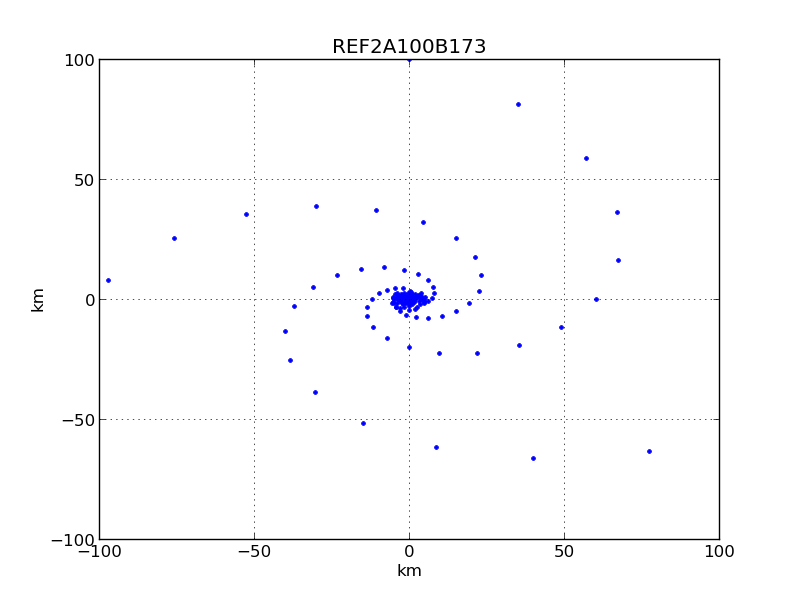
\includegraphics[width=0.150000\textwidth,trim= 0 .05cm 0 0.05cm]{{images/lay_SKA1REF2}.png} &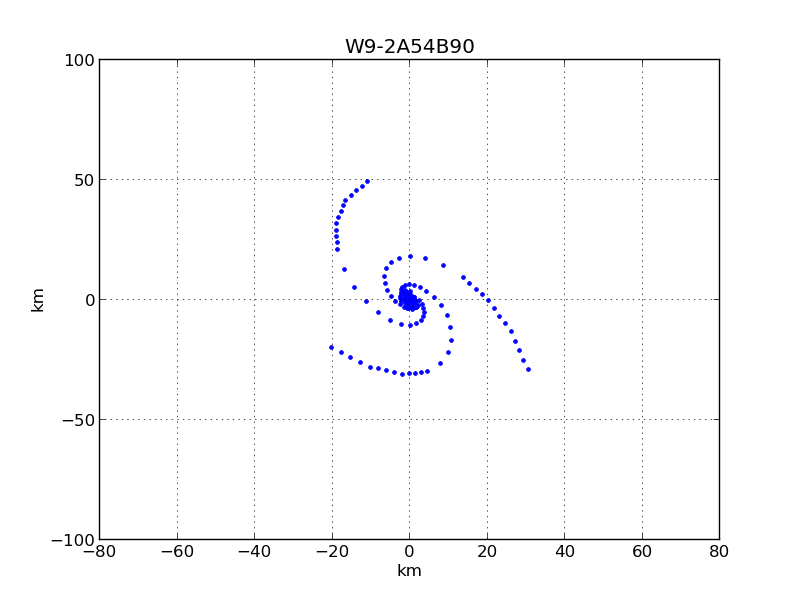
\includegraphics[width=0.150000\textwidth,trim= 0 .05cm 0 0.05cm]{{images/lay_SKA1W9-12A54B90}.png} &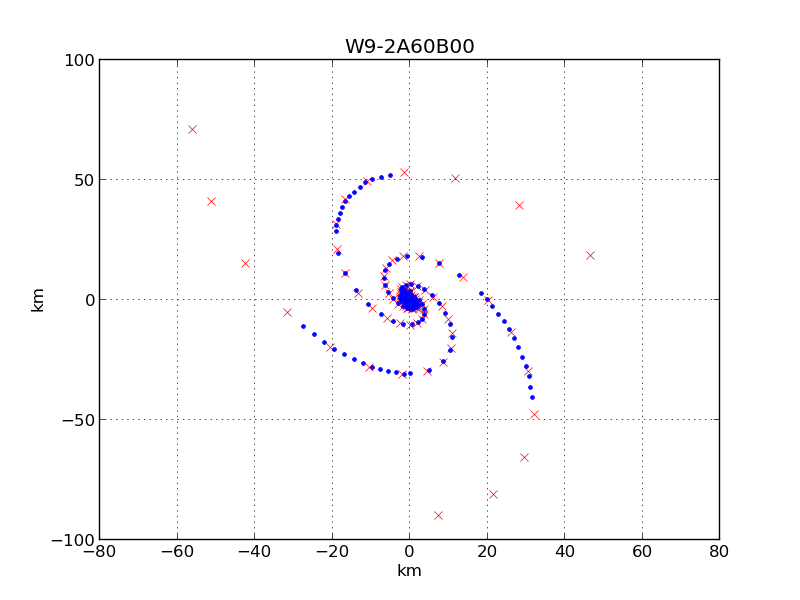
\includegraphics[width=0.150000\textwidth,trim= 0 .05cm 0 0.05cm]{{images/lay_SKA1W9-12A60B100}.png} &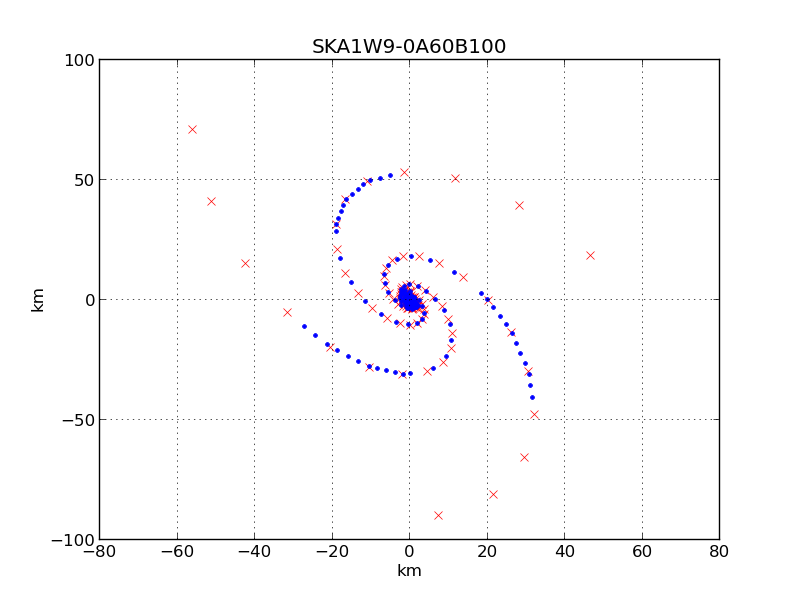
\includegraphics[width=0.150000\textwidth,trim= 0 .05cm 0 0.05cm]{{images/lay_SKA1W9-0A60B100}.png} &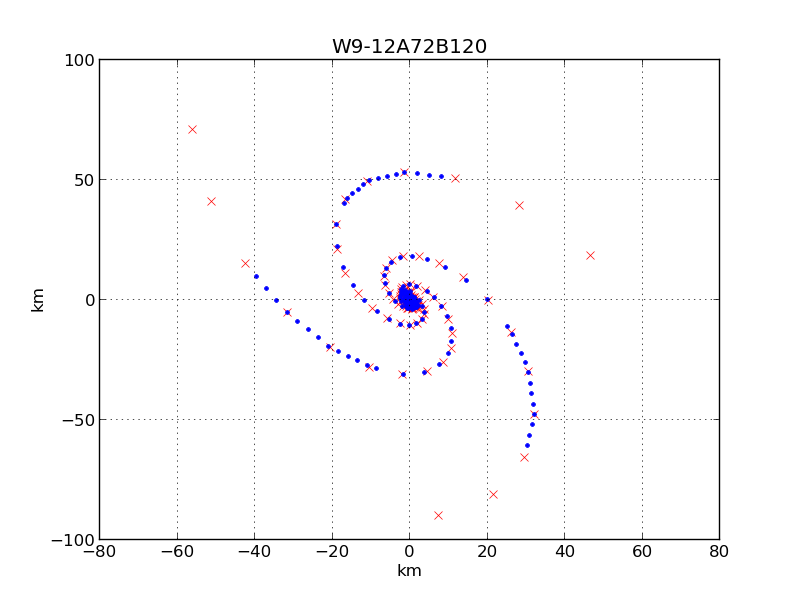
\includegraphics[width=0.150000\textwidth,trim= 0 .05cm 0 0.05cm]{{images/lay_SKA1W9-12A72B120}.png} &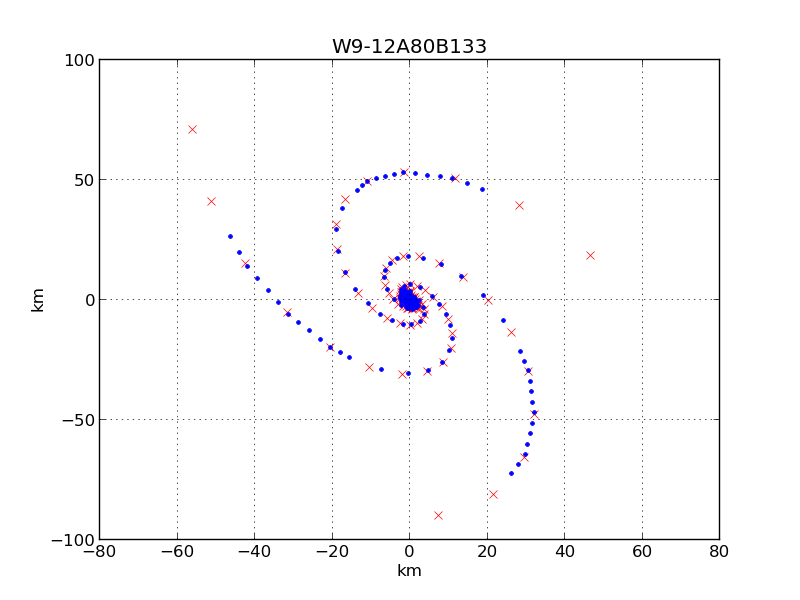
\includegraphics[width=0.150000\textwidth,trim= 0 .05cm 0 0.05cm]{{images/lay_SKA1W9-12A80B133}.png} 
 \\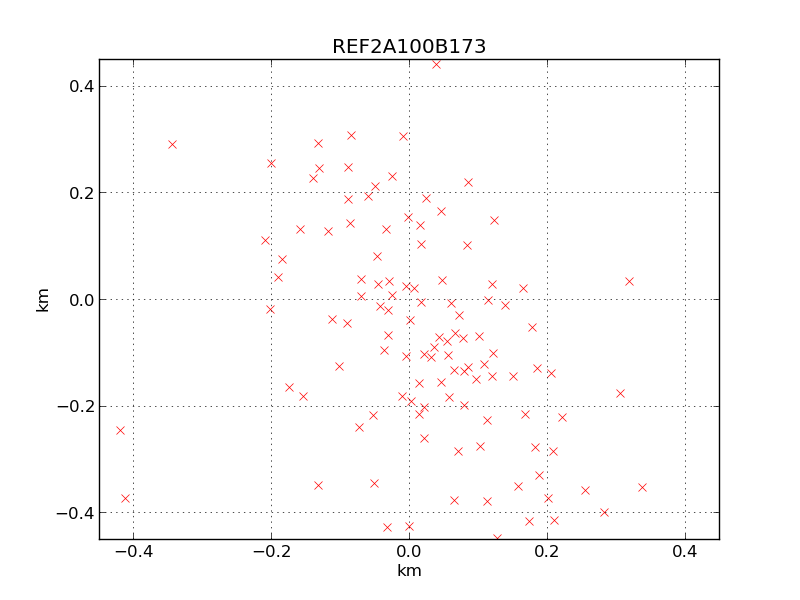
\includegraphics[width=0.150000\textwidth,trim= 0 .05cm 0 0.05cm]{{images/core_SKA1REF2}.png} &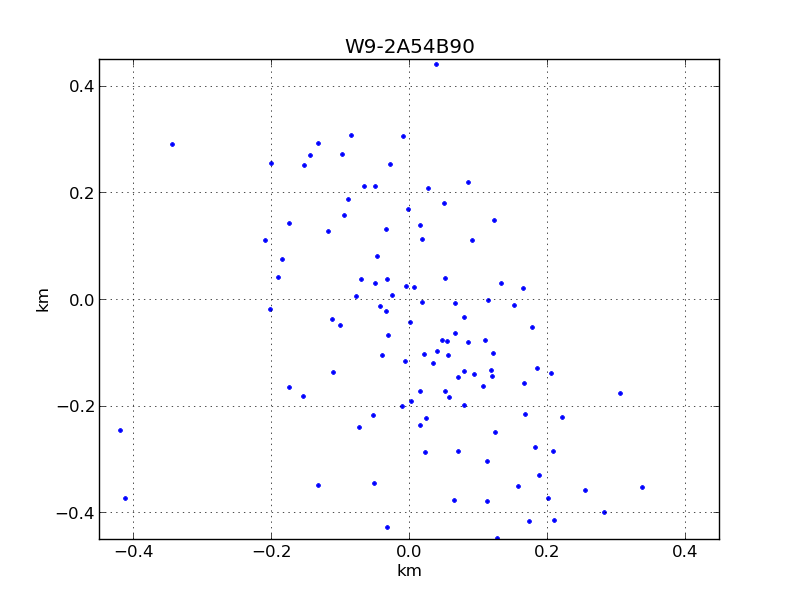
\includegraphics[width=0.150000\textwidth,trim= 0 .05cm 0 0.05cm]{{images/core_SKA1W9-12A54B90}.png} &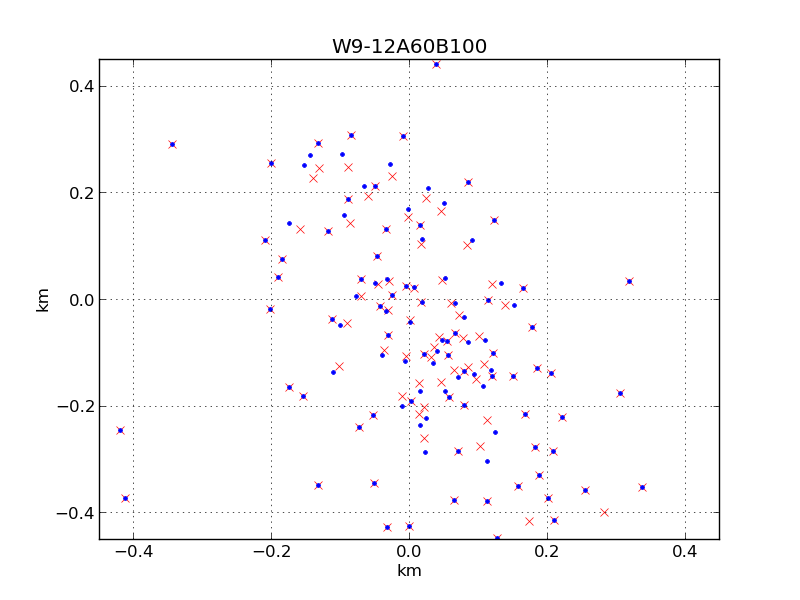
\includegraphics[width=0.150000\textwidth,trim= 0 .05cm 0 0.05cm]{{images/core_SKA1W9-12A60B100}.png} &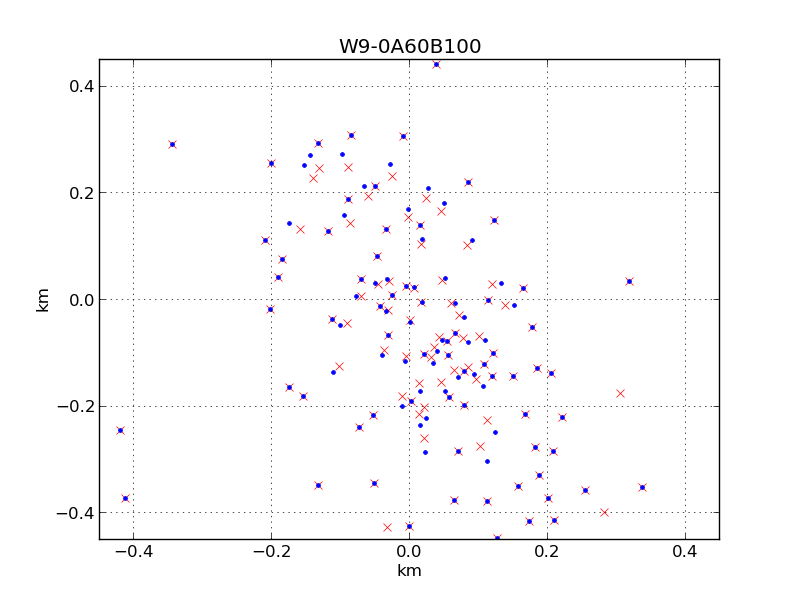
\includegraphics[width=0.150000\textwidth,trim= 0 .05cm 0 0.05cm]{{images/core_SKA1W9-0A60B100}.png} &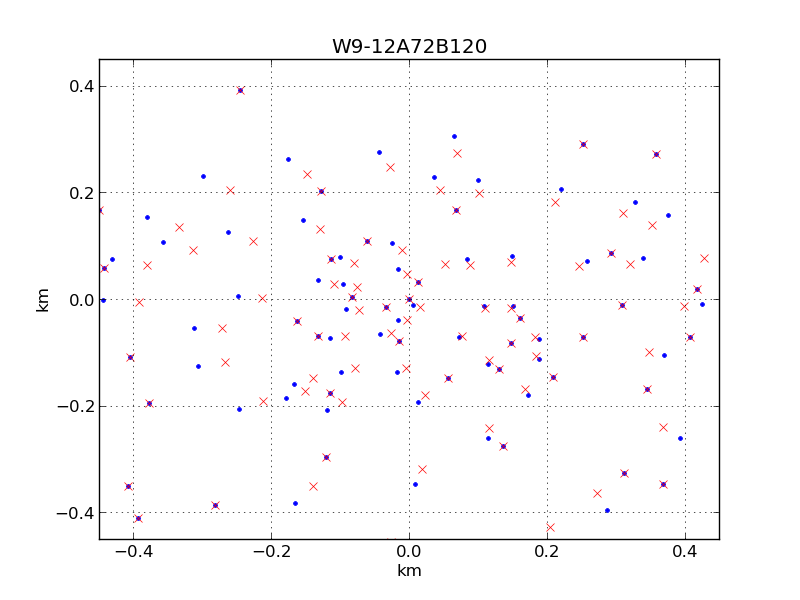
\includegraphics[width=0.150000\textwidth,trim= 0 .05cm 0 0.05cm]{{images/core_SKA1W9-12A72B120}.png} &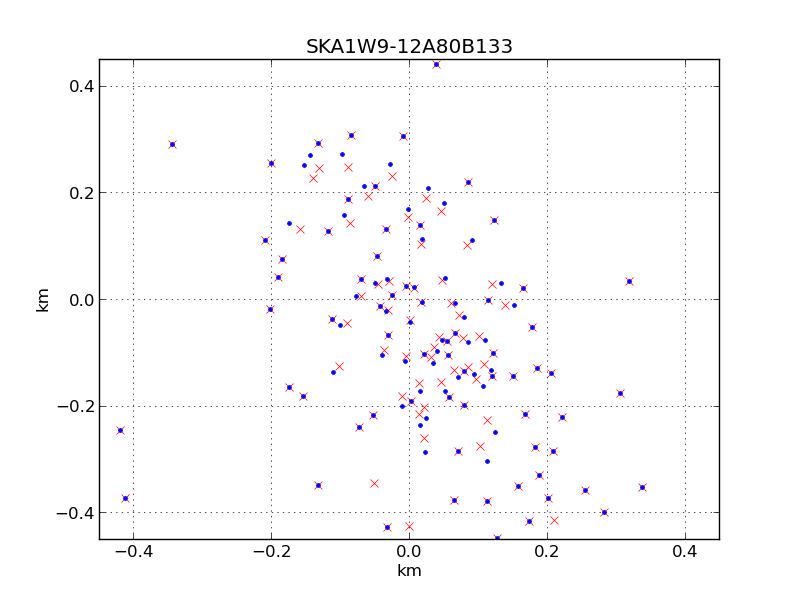
\includegraphics[width=0.150000\textwidth,trim= 0 .05cm 0 0.05cm]{{images/core_SKA1W9-12A80B133}.png} 
 \\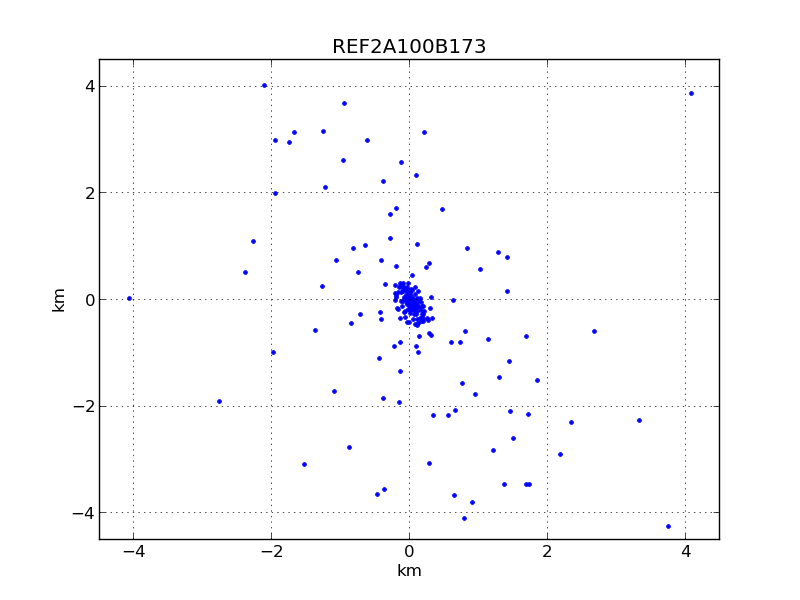
\includegraphics[width=0.150000\textwidth,trim= 0 .05cm 0 0.05cm]{{images/outer_core_SKA1REF2}.png} &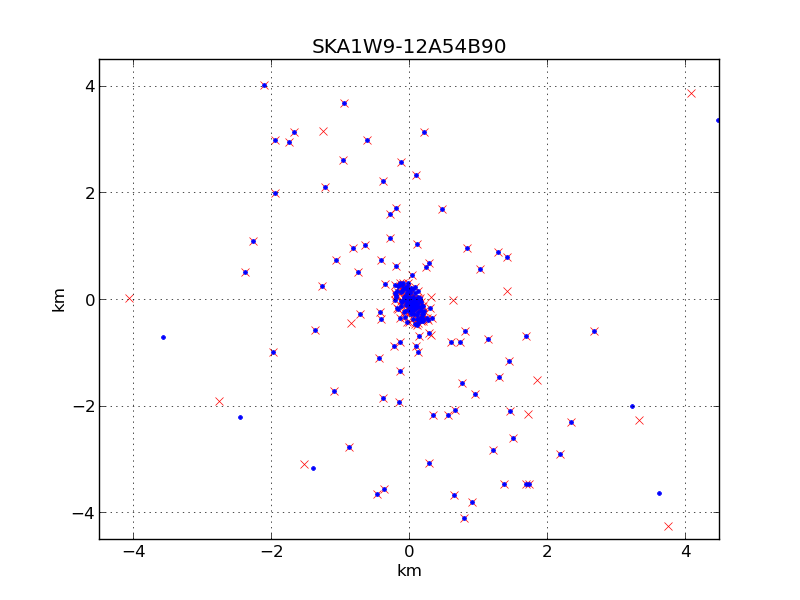
\includegraphics[width=0.150000\textwidth,trim= 0 .05cm 0 0.05cm]{{images/outer_core_SKA1W9-12A54B90}.png} &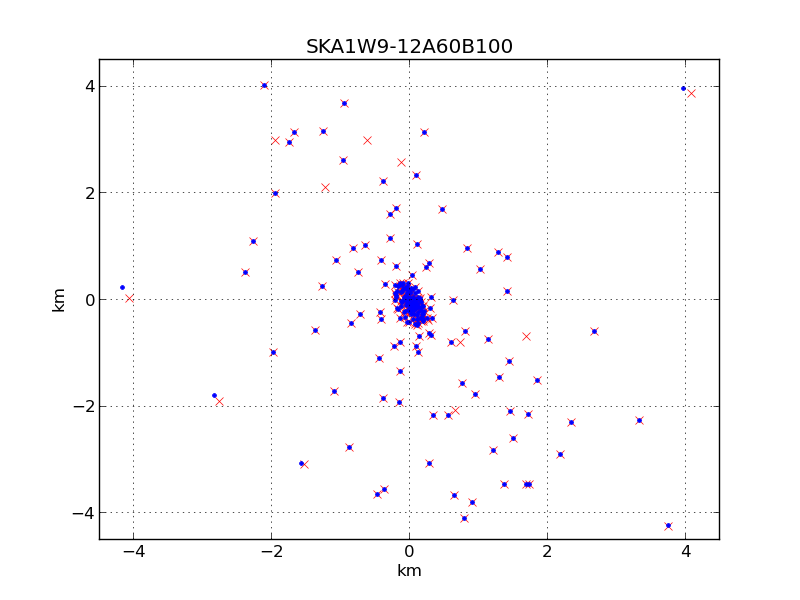
\includegraphics[width=0.150000\textwidth,trim= 0 .05cm 0 0.05cm]{{images/outer_core_SKA1W9-12A60B100}.png} &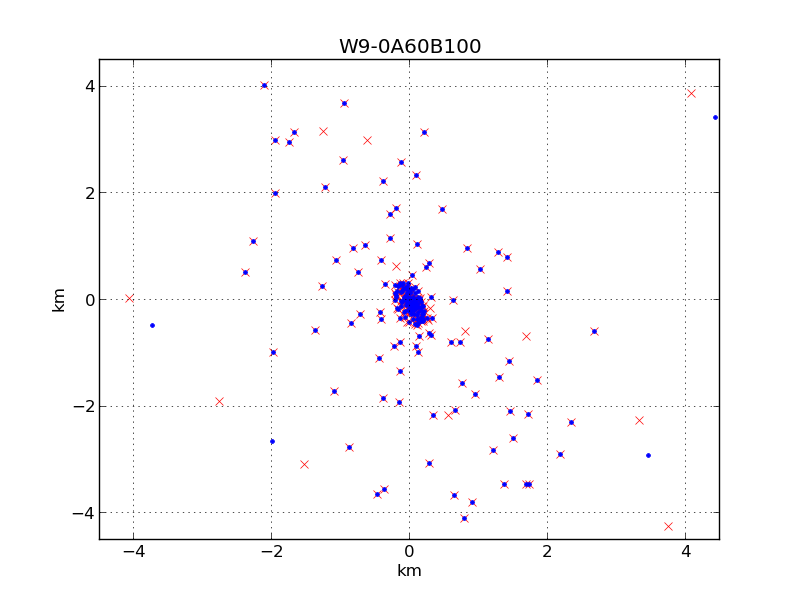
\includegraphics[width=0.150000\textwidth,trim= 0 .05cm 0 0.05cm]{{images/outer_core_SKA1W9-0A60B100}.png} &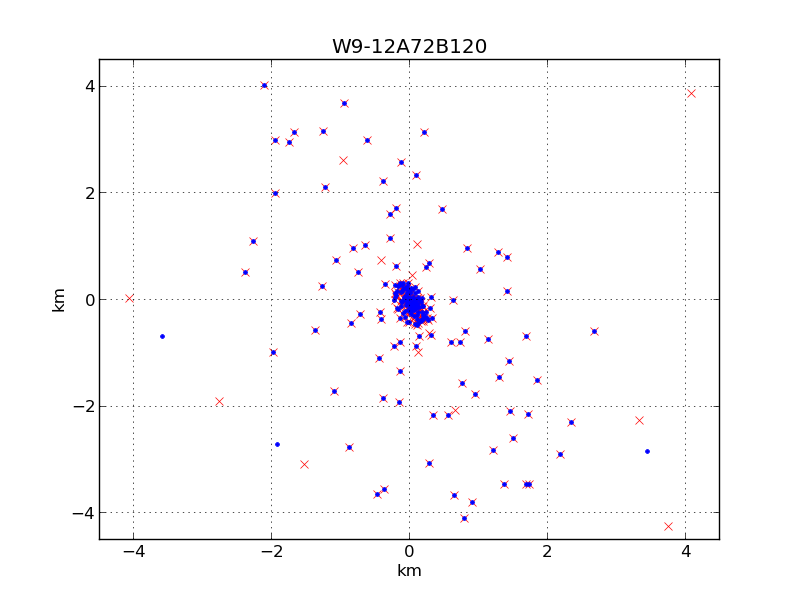
\includegraphics[width=0.150000\textwidth,trim= 0 .05cm 0 0.05cm]{{images/outer_core_SKA1W9-12A72B120}.png} &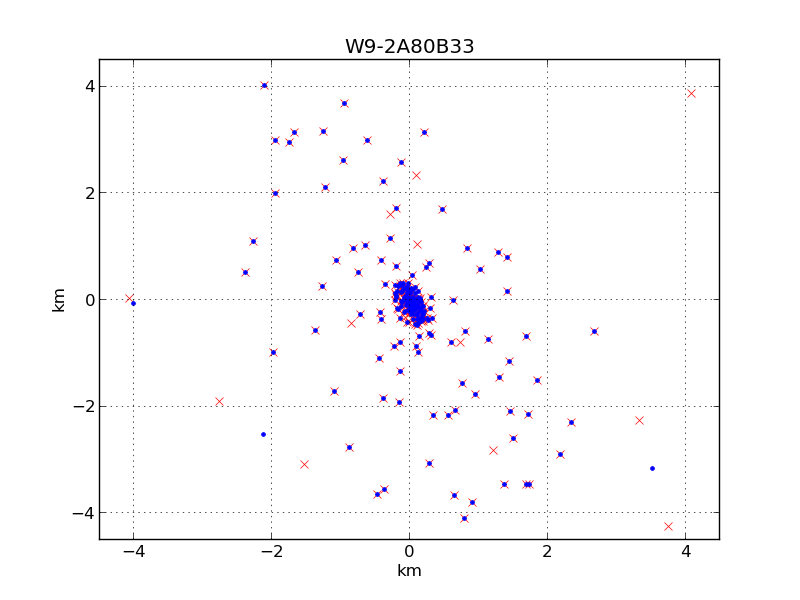
\includegraphics[width=0.150000\textwidth,trim= 0 .05cm 0 0.05cm]{{images/outer_core_SKA1W9-12A80B133}.png} 
 \\\end{tabular}}
 \caption{Antenna layouts, REF2 plotted as a reference (red crosses)}\label{fig:lay}
\end{figure}
% baseline distribution histograms
\begin{figure}[H]
 \tiny{%%% autogen
 \begin{tabular}{lllll}
\includegraphics[width=0.180000\textwidth,trim= 0 .05cm 0 0.05cm]{{}.images/hist*REF2png} &\includegraphics[width=0.180000\textwidth,trim= 0 .05cm 0 0.05cm]{{}.images/hist*W9-12A72png} &\includegraphics[width=0.180000\textwidth,trim= 0 .05cm 0 0.05cm]{{}.images/hist*W9-0A72png} &\includegraphics[width=0.180000\textwidth,trim= 0 .05cm 0 0.05cm]{{}.images/hist*SUR1png} &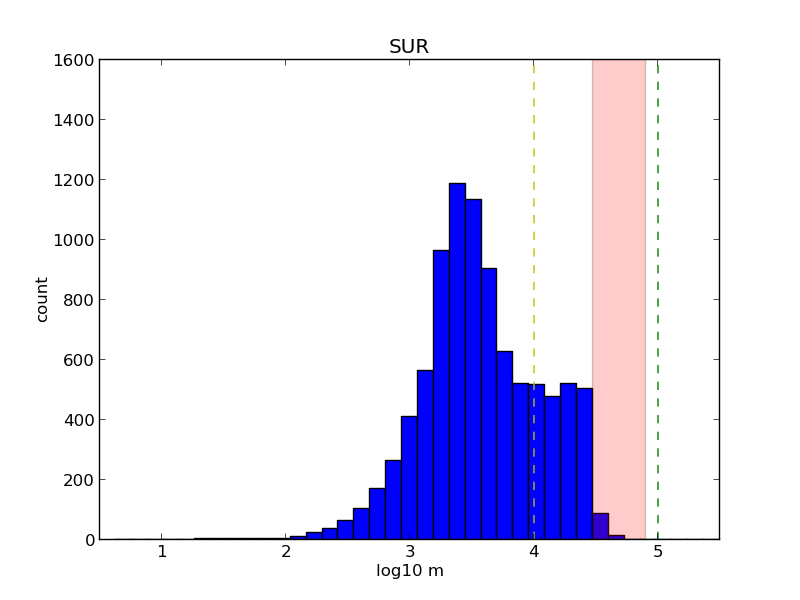
\includegraphics[width=0.180000\textwidth,trim= 0 .05cm 0 0.05cm]{{images/hist_SKASUR}.png} 
 \\ \hfill\end{tabular}}
 \caption{Baseline distribution with the uv-distance in $log_{10}$ km . Yellow and green dashed lines mark 10 and 120
kilometres respectively, and the pink strip represents baselines from 30-80km.}\label{fig:hist}
\end{figure}

% uv-coverage plots 
\begin{figure}[H]
 \tiny{%auto gen
\begin{tabular}{ccccc}
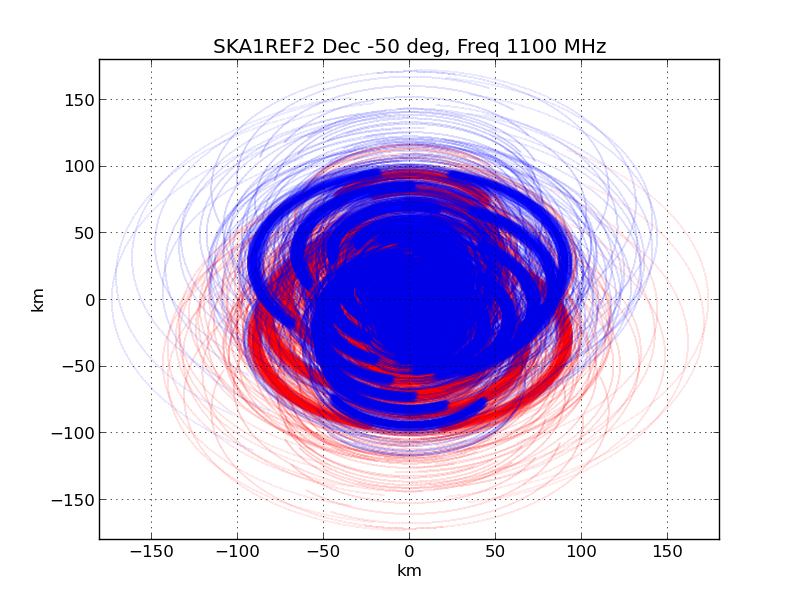
\includegraphics[width=0.180000\textwidth,trim= 0 .05cm 0 0.05cm]{{images/uvcov_SKA1REF2_-50_1100}.png} &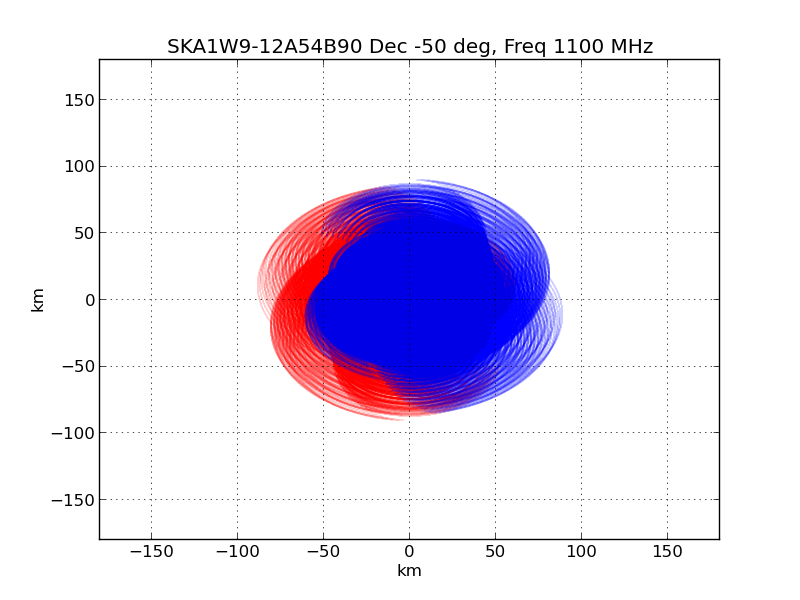
\includegraphics[width=0.180000\textwidth,trim= 0 .05cm 0 0.05cm]{{images/uvcov_SKA1W9-12A54B90_-50_1100}.png} &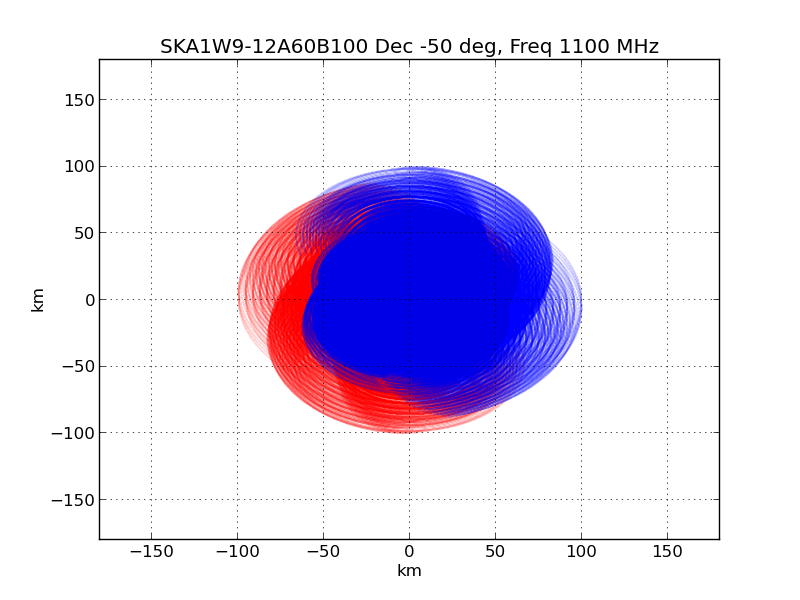
\includegraphics[width=0.180000\textwidth,trim= 0 .05cm 0 0.05cm]{{images/uvcov_SKA1W9-12A60B100_-50_1100}.png} &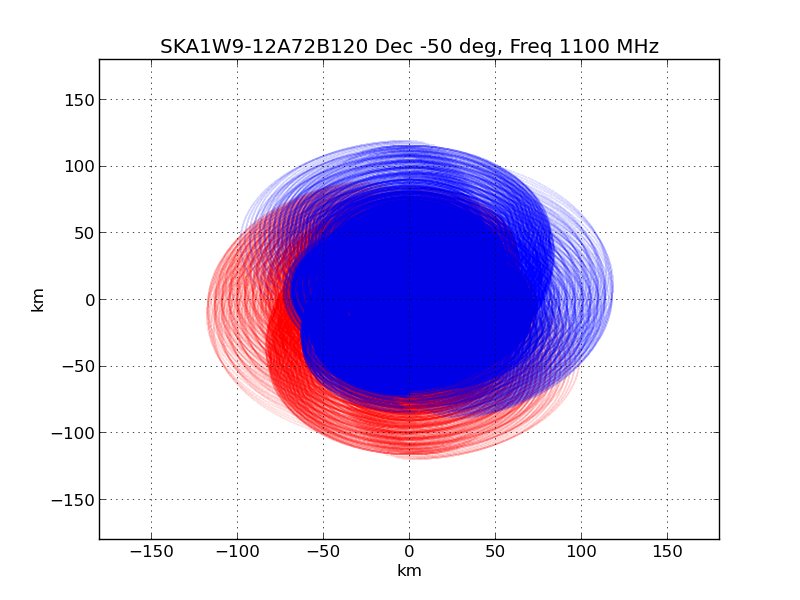
\includegraphics[width=0.180000\textwidth,trim= 0 .05cm 0 0.05cm]{{images/uvcov_SKA1W9-12A72B120_-50_1100}.png} &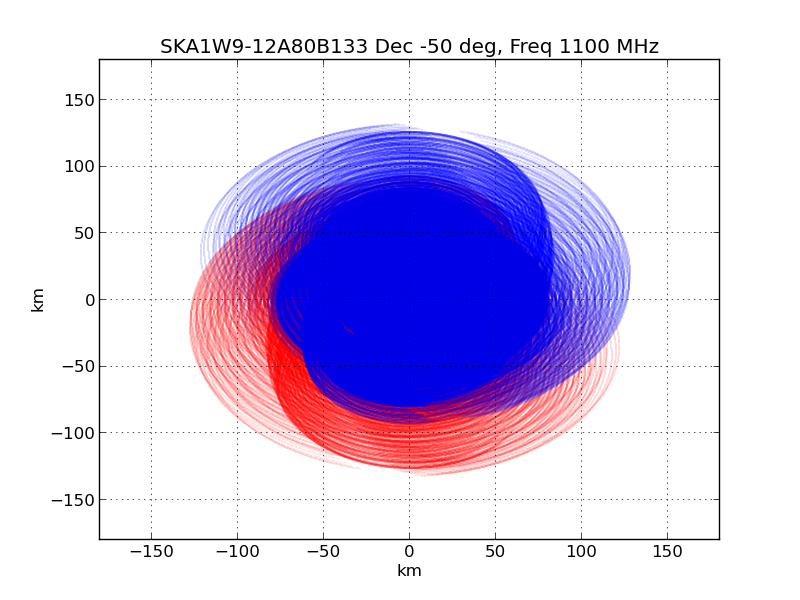
\includegraphics[width=0.180000\textwidth,trim= 0 .05cm 0 0.05cm]{{images/uvcov_SKA1W9-12A80B133_-50_1100}.png} \\
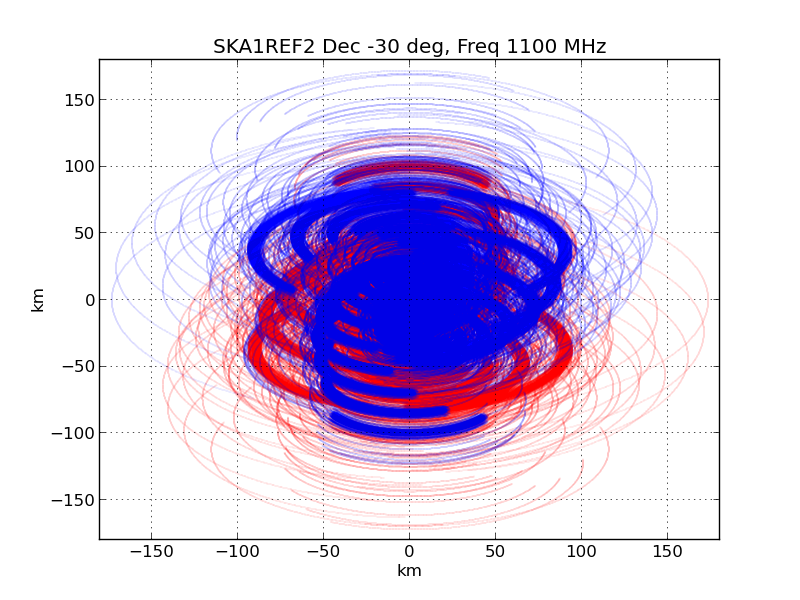
\includegraphics[width=0.180000\textwidth,trim= 0 .05cm 0 0.05cm]{{images/uvcov_SKA1REF2_-30_1100}.png} &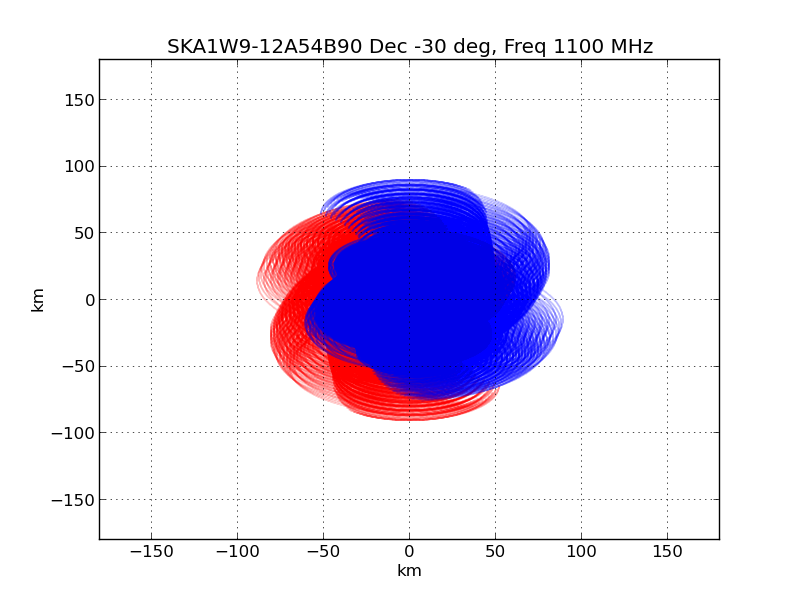
\includegraphics[width=0.180000\textwidth,trim= 0 .05cm 0 0.05cm]{{images/uvcov_SKA1W9-12A54B90_-30_1100}.png} &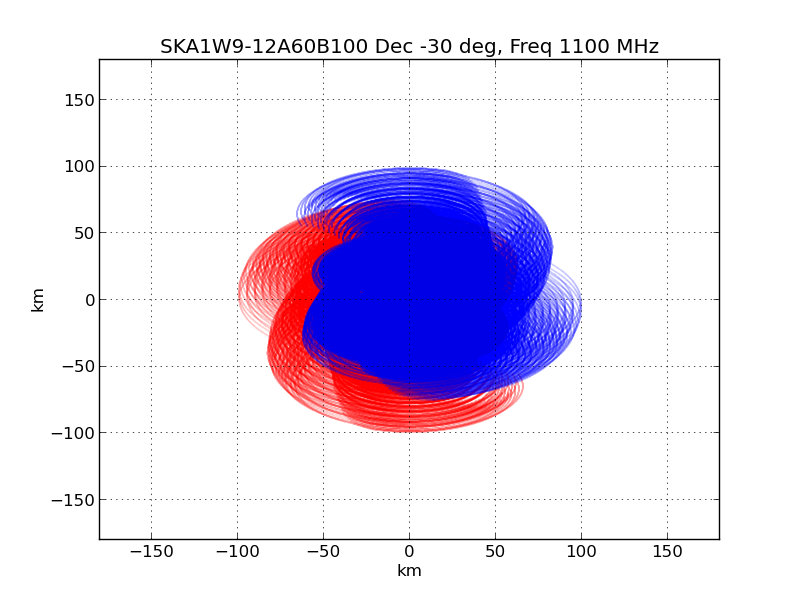
\includegraphics[width=0.180000\textwidth,trim= 0 .05cm 0 0.05cm]{{images/uvcov_SKA1W9-12A60B100_-30_1100}.png} &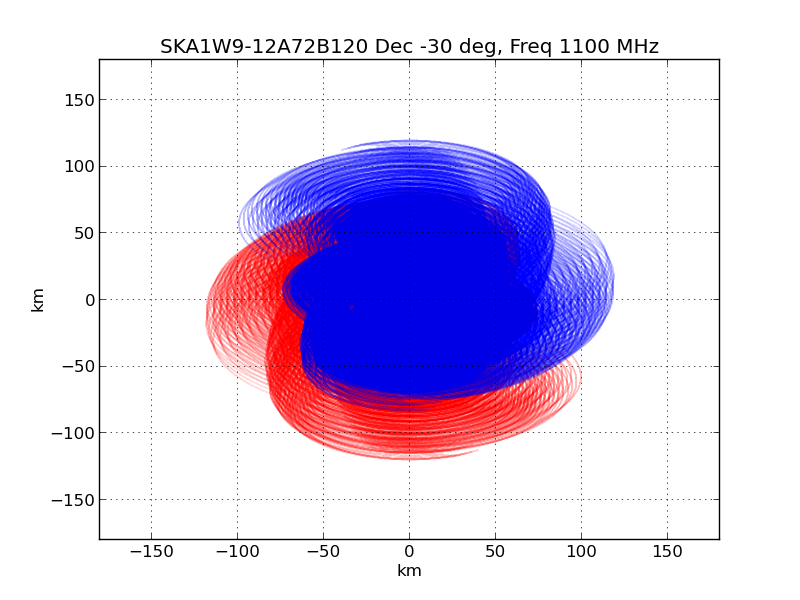
\includegraphics[width=0.180000\textwidth,trim= 0 .05cm 0 0.05cm]{{images/uvcov_SKA1W9-12A72B120_-30_1100}.png} &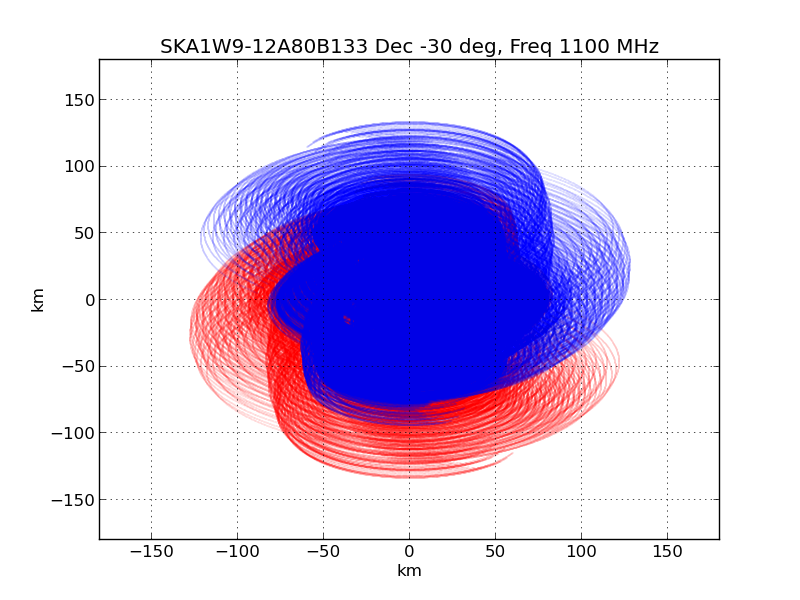
\includegraphics[width=0.180000\textwidth,trim= 0 .05cm 0 0.05cm]{{images/uvcov_SKA1W9-12A80B133_-30_1100}.png} \\
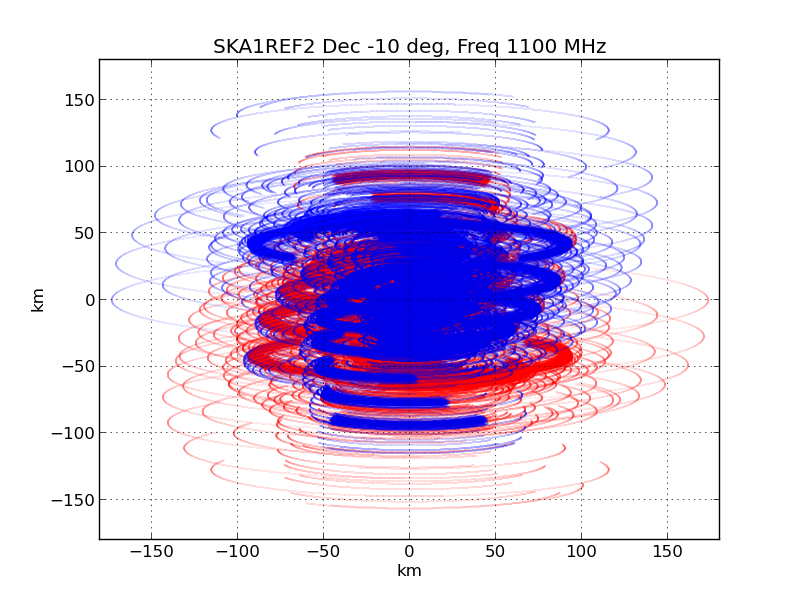
\includegraphics[width=0.180000\textwidth,trim= 0 .05cm 0 0.05cm]{{images/uvcov_SKA1REF2_-10_1100}.png} &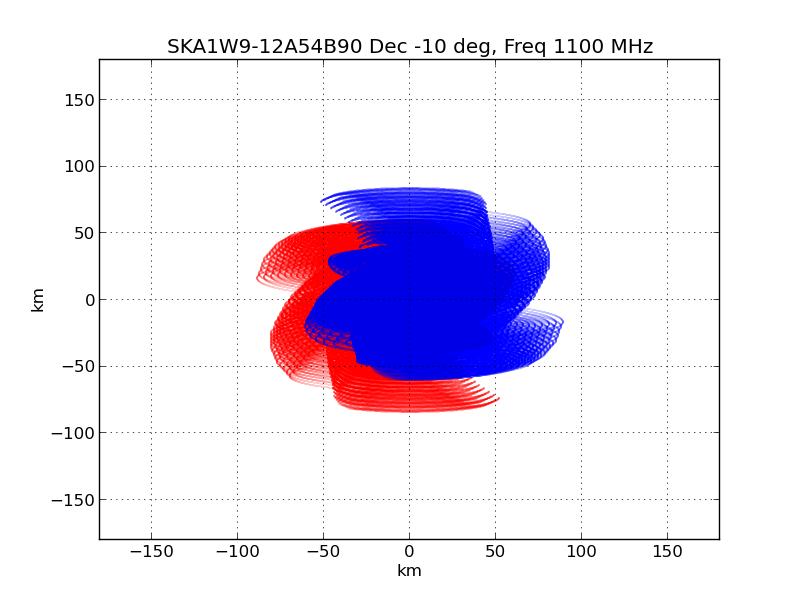
\includegraphics[width=0.180000\textwidth,trim= 0 .05cm 0 0.05cm]{{images/uvcov_SKA1W9-12A54B90_-10_1100}.png} &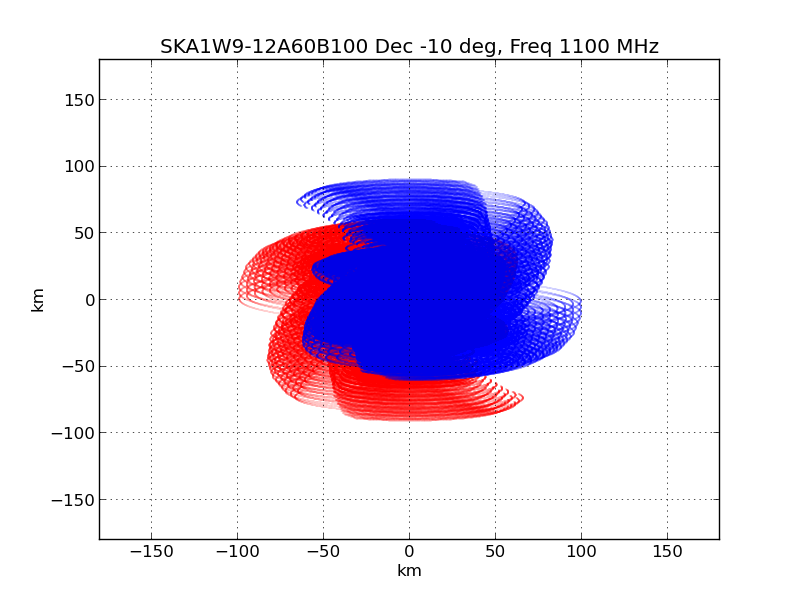
\includegraphics[width=0.180000\textwidth,trim= 0 .05cm 0 0.05cm]{{images/uvcov_SKA1W9-12A60B100_-10_1100}.png} &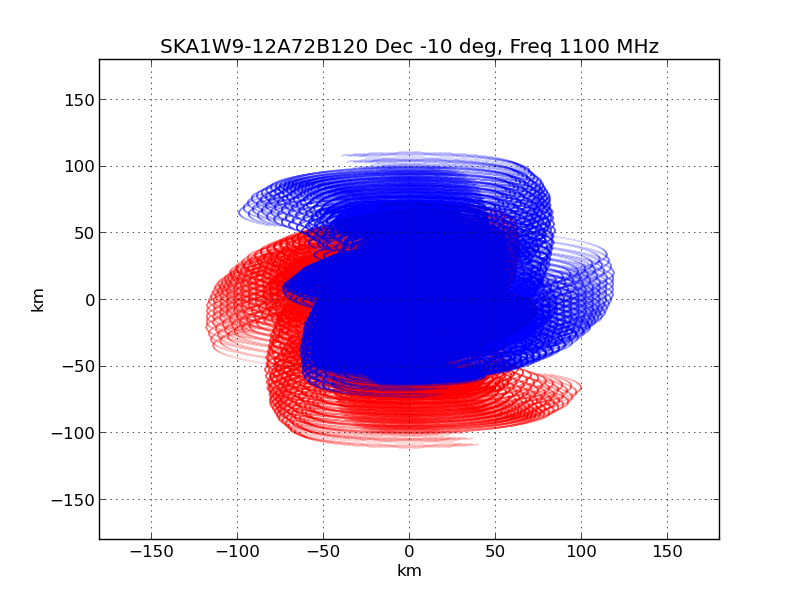
\includegraphics[width=0.180000\textwidth,trim= 0 .05cm 0 0.05cm]{{images/uvcov_SKA1W9-12A72B120_-10_1100}.png} &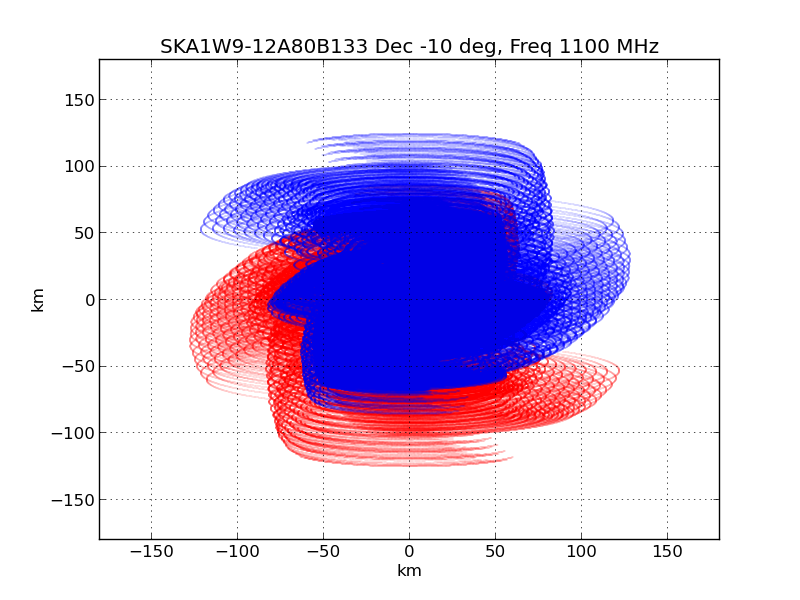
\includegraphics[width=0.180000\textwidth,trim= 0 .05cm 0 0.05cm]{{images/uvcov_SKA1W9-12A80B133_-10_1100}.png} 
\end{tabular}}
 \caption{UV-Coverage for 8-hr tracks at 1.1 GHz (50MHz bandwidth) at declinations -50,-30,-10 for the different layouts. Blue
indicates uv-points, red indicates conjugate uv-points.}\label{fig:uvcov}
\end{figure}

\section{The Experiment}\label{sec:exp}
Our aim is to investigate the scale-dependent sensitivity of the layouts described in the previous section.
We use the \texttt{makems} tool to make simulated measurement sets of 8hr tracks with a 60s integration time on declinations
\{-50, -30, -10\} degrees at frequencies of \{650, 800, 1100\}MHz with a single 50MHz channel. The expected rms noise per real
and imaginary part for each visibility is calculated as 
\begin{equation}
\sigma_{\text{vis}} = \frac{\text{SEFD}}{\sqrt{2\Delta t\Delta \nu}}.
\end{equation}
We use the baseline designs SEFD value of 400 corresponding to the 15 m dishes. We then fill the MS with random Gaussian noise
using the computed value of the noise for a given integration and bandwidth. We then use the (CASA-derived) \texttt{lwimager} tool
to make maps of the PSF as well as dirty maps of the noise using various weighting schemes. Note that for uniform and robust
weighting, a crucial parameter is the size of the uv-bin over which weights are “uniformized”. By default this is determined from
the full image size, but \texttt{lwimager} allows one to uniformize the weights over bins corresponding to a user-defined FoV
instead. For these simulations uv-bins corresponding to a FoV of 10 arcmin were used. The following metrics were generated:\\ {\bf
Note:} These metrics are generated at different angular scales, this is done by applying an inner-taper\footnote{The weights for
the taper are generated using a Butterworth function.} to taper out baselines that do not fall within a given resolution range,
i.e., we only consider uv-points that correspond to a given resolution.
\begin{itemize}
 \item PSF full width at hafl maximum (FWHM) size (mean of the FWHM dimensions). This was measured by making high-resolution
images of the PSF (0.05 arcsec
resolution), and fitting a Gaussian to the PSF. Note that for the highly non-Gaussian PSFs corresponding to natural and (some)
robust weighting schemes, the fit is very poor, so the size parameter becomes somewhat ill-defined (Table \ref{tab:psf_mean}).
A catalog of PSF cross-sections is provided in Appendix \ref{app:psf}

 \item PSF symmetry (PSF size parameters are obtained as explained above). As a measure of PSF symmetry, we define 
$\text{PSF}_{sym}=1-\text{FWHM}_{min}/\text{FWHM}_{maj}$, then $\text{PSF}_{sym} = 0$ is perfect symmetry, and the symmetry
degenerates as $\text{PSF}_{sym}\,\,\, \rightarrow\,\,1$ (Table \ref{tab:psf_sym}).

 \item Rms pixel noise at different angular scales for 50 and 166MHz wide bands (Tables \ref{tab:noise50} and \ref{tab:noise166}).
 
 \item SNR for a 10$\mu$Jy source at 1100MHz with a spectral index of -0.7 after 8hrs for a 166MHz band (Table \ref{tab:snr10}).
 \item Average SNR over frequencies 650, 800 and 1100MHz (166MHz band)
   after 8 hours, for a 10$\mu$Jy source at 1100MHz
with a spectral index of -0.7 (Table \ref{tab:snravg}). {$\overline{SNR10}=\sqrt{SNR10_{650}^2 + SNR10_{800}^2 +
SNR10_{1100}^2}$}.
 \item Hours required to reach a mean SNR of 10 (Table \ref{tab:hours}).
\end{itemize}
% \section{Results}\label{sec:results}
%===========================================================Performance Stats===============================================
% Auto generated table
 \vspace{-4cm}\begin{table}[H]
 \tiny{\subfloat[DEC=-10, natural weighting]{\begin{tabular}{|lccccc||ccccc||ccccc|} 
 \\ \cline{2-16} \multicolumn{1}{c}{ } & \multicolumn{5}{|c}{650MHz}  & \multicolumn{5}{c}{800MHz}  & \multicolumn{5}{c|}{1100MHz} \\ \cline{1-16} 
 resbin  &1 & 2 & 3 & 4 & 5 & 1 & 2 & 3 & 4 & 5 & 1 & 2 & 3 & 4 & 5 \\ \hline
SKA1REF2 & 0.65 \cellcolor{blue!18.00} & 1.33 \cellcolor{red!60.00} & 2.33 \cellcolor{green!39.98} & 3.35 \cellcolor{orange!60.00} & 803.08 \cellcolor{purple!60.00} & 0.60 \cellcolor{blue!18.00} & 1.33 \cellcolor{red!60.00} & 2.35 \cellcolor{green!25.87} & 3.34 \cellcolor{orange!59.86} & 792.32 \cellcolor{purple!60.00} & 0.59 \cellcolor{blue!31.03} & 1.33 \cellcolor{red!60.00} & 2.35 \cellcolor{green!58.67} & 3.35 \cellcolor{orange!60.00} & 763.61 \cellcolor{purple!21.13}\\ \hline 
SKA1W9-12A54B90 & 0.85 \cellcolor{blue!60.00} & 1.29 \cellcolor{red!43.04} & 2.32 \cellcolor{green!18.00} & 3.34 \cellcolor{orange!42.46} & 794.44 \cellcolor{purple!18.00} & 0.81 \cellcolor{blue!60.00} & 1.24 \cellcolor{red!24.52} & 2.35 \cellcolor{green!33.00} & 3.33 \cellcolor{orange!51.52} & 790.43 \cellcolor{purple!26.76} & 0.69 \cellcolor{blue!60.00} & 1.28 \cellcolor{red!18.00} & 2.34 \cellcolor{green!49.15} & 3.33 \cellcolor{orange!29.35} & 767.45 \cellcolor{purple!56.57}\\ \hline 
SKA1W9-12A60B100 & 0.84 \cellcolor{blue!56.59} & 1.25 \cellcolor{red!27.98} & 2.32 \cellcolor{green!21.46} & 3.33 \cellcolor{orange!22.95} & 796.90 \cellcolor{purple!29.96} & 0.77 \cellcolor{blue!53.01} & 1.23 \cellcolor{red!22.55} & 2.36 \cellcolor{green!60.00} & 3.34 \cellcolor{orange!60.00} & 789.93 \cellcolor{purple!18.00} & 0.64 \cellcolor{blue!47.03} & 1.30 \cellcolor{red!34.41} & 2.34 \cellcolor{green!53.44} & 3.34 \cellcolor{orange!35.19} & 767.82 \cellcolor{purple!60.00}\\ \hline 
SKA1W9-0A60B100 & 0.84 \cellcolor{blue!57.47} & 1.24 \cellcolor{red!24.63} & 2.33 \cellcolor{green!40.13} & 3.35 \cellcolor{orange!57.03} & 797.66 \cellcolor{purple!33.66} & 0.78 \cellcolor{blue!53.72} & 1.22 \cellcolor{red!18.00} & 2.36 \cellcolor{green!46.12} & 3.32 \cellcolor{orange!46.61} & 791.83 \cellcolor{purple!51.53} & 0.64 \cellcolor{blue!46.86} & 1.30 \cellcolor{red!37.75} & 2.35 \cellcolor{green!60.00} & 3.33 \cellcolor{orange!18.00} & 765.46 \cellcolor{purple!38.18}\\ \hline 
SKA1W9-12A72B120 & 0.78 \cellcolor{blue!44.81} & 1.22 \cellcolor{red!18.00} & 2.35 \cellcolor{green!60.00} & 3.35 \cellcolor{orange!47.70} & 798.73 \cellcolor{purple!38.85} & 0.70 \cellcolor{blue!39.05} & 1.28 \cellcolor{red!40.29} & 2.35 \cellcolor{green!18.00} & 3.32 \cellcolor{orange!43.73} & 790.38 \cellcolor{purple!26.03} & 0.57 \cellcolor{blue!25.70} & 1.32 \cellcolor{red!52.95} & 2.32 \cellcolor{green!37.83} & 3.33 \cellcolor{orange!27.41} & 763.27 \cellcolor{purple!18.00}\\ \hline 
SKA1W9-12A80B133 & 0.74 \cellcolor{blue!36.60} & 1.25 \cellcolor{red!27.03} & 2.34 \cellcolor{green!42.99} & 3.32 \cellcolor{orange!18.00} & 797.36 \cellcolor{purple!32.22} & 0.65 \cellcolor{blue!29.03} & 1.30 \cellcolor{red!47.47} & 2.36 \cellcolor{green!57.00} & 3.28 \cellcolor{orange!18.00} & 790.65 \cellcolor{purple!30.63} & 0.54 \cellcolor{blue!18.00} & 1.32 \cellcolor{red!54.72} & 2.30 \cellcolor{green!18.00} & 3.33 \cellcolor{orange!28.22} & 767.22 \cellcolor{purple!54.47}\\ \hline 
\end{tabular}}
\vspace{-0.300000cm}
\hspace{1cm} 
\subfloat[DEC=-10, robust-2 weighting ]{\begin{tabular}{|lccccc||ccccc||ccccc|} 
 \\ \cline{2-16} \multicolumn{1}{c}{ } & \multicolumn{5}{|c}{650MHz}  & \multicolumn{5}{c}{800MHz}  & \multicolumn{5}{c|}{1100MHz} \\ \cline{1-16} 
 resbin  &1 & 2 & 3 & 4 & 5 & 1 & 2 & 3 & 4 & 5 & 1 & 2 & 3 & 4 & 5 \\ \hline
SKA1REF2 & 0.73 \cellcolor{blue!20.97} & 1.22 \cellcolor{red!60.00} & 2.25 \cellcolor{green!60.00} & 3.26 \cellcolor{orange!60.00} & 745.23 \cellcolor{purple!60.00} & 0.62 \cellcolor{blue!19.20} & 1.21 \cellcolor{red!60.00} & 2.24 \cellcolor{green!60.00} & 3.25 \cellcolor{orange!54.15} & 791.85 \cellcolor{purple!60.00} & 0.53 \cellcolor{blue!25.74} & 1.19 \cellcolor{red!60.00} & 2.24 \cellcolor{green!48.77} & 3.26 \cellcolor{orange!42.50} & 761.50 \cellcolor{purple!18.00}\\ \hline 
SKA1W9-12A54B90 & 0.96 \cellcolor{blue!60.00} & 1.22 \cellcolor{red!54.94} & 2.23 \cellcolor{green!18.00} & 3.25 \cellcolor{orange!37.87} & 732.34 \cellcolor{purple!18.00} & 0.78 \cellcolor{blue!60.00} & 1.16 \cellcolor{red!30.00} & 2.23 \cellcolor{green!18.00} & 3.25 \cellcolor{orange!53.62} & 790.56 \cellcolor{purple!33.85} & 0.59 \cellcolor{blue!60.00} & 1.15 \cellcolor{red!18.00} & 2.24 \cellcolor{green!36.71} & 3.25 \cellcolor{orange!33.27} & 766.98 \cellcolor{purple!57.61}\\ \hline 
SKA1W9-12A60B100 & 0.88 \cellcolor{blue!46.78} & 1.19 \cellcolor{red!36.63} & 2.23 \cellcolor{green!28.20} & 3.25 \cellcolor{orange!38.62} & 735.91 \cellcolor{purple!29.65} & 0.72 \cellcolor{blue!45.46} & 1.16 \cellcolor{red!23.49} & 2.24 \cellcolor{green!32.73} & 3.25 \cellcolor{orange!54.68} & 789.78 \cellcolor{purple!18.00} & 0.57 \cellcolor{blue!47.57} & 1.16 \cellcolor{red!24.36} & 2.24 \cellcolor{green!43.37} & 3.25 \cellcolor{orange!32.00} & 767.31 \cellcolor{purple!60.00}\\ \hline 
SKA1W9-0A60B100 & 0.90 \cellcolor{blue!49.50} & 1.19 \cellcolor{red!38.48} & 2.24 \cellcolor{green!39.09} & 3.26 \cellcolor{orange!43.15} & 735.17 \cellcolor{purple!27.24} & 0.74 \cellcolor{blue!49.02} & 1.16 \cellcolor{red!24.43} & 2.24 \cellcolor{green!41.51} & 3.25 \cellcolor{orange!60.00} & 791.68 \cellcolor{purple!56.61} & 0.58 \cellcolor{blue!53.60} & 1.16 \cellcolor{red!28.42} & 2.24 \cellcolor{green!60.00} & 3.25 \cellcolor{orange!25.32} & 763.98 \cellcolor{purple!35.90}\\ \hline 
SKA1W9-12A72B120 & 0.77 \cellcolor{blue!28.28} & 1.16 \cellcolor{red!21.39} & 2.24 \cellcolor{green!42.02} & 3.25 \cellcolor{orange!39.38} & 736.00 \cellcolor{purple!29.93} & 0.64 \cellcolor{blue!25.58} & 1.15 \cellcolor{red!18.00} & 2.24 \cellcolor{green!34.61} & 3.25 \cellcolor{orange!27.57} & 790.19 \cellcolor{purple!26.29} & 0.53 \cellcolor{blue!29.37} & 1.17 \cellcolor{red!36.24} & 2.23 \cellcolor{green!18.00} & 3.25 \cellcolor{orange!18.00} & 761.79 \cellcolor{purple!20.11}\\ \hline 
SKA1W9-12A80B133 & 0.71 \cellcolor{blue!18.00} & 1.16 \cellcolor{red!18.00} & 2.24 \cellcolor{green!45.31} & 3.25 \cellcolor{orange!18.00} & 734.91 \cellcolor{purple!26.39} & 0.61 \cellcolor{blue!18.00} & 1.15 \cellcolor{red!20.31} & 2.23 \cellcolor{green!30.54} & 3.25 \cellcolor{orange!18.00} & 790.41 \cellcolor{purple!30.68} & 0.51 \cellcolor{blue!18.00} & 1.17 \cellcolor{red!39.68} & 2.23 \cellcolor{green!20.50} & 3.26 \cellcolor{orange!60.00} & 766.24 \cellcolor{purple!52.27}\\ \hline 
\end{tabular}}
\vspace{-0.300000cm}
\hspace{1cm} 
\subfloat[DEC=-10, robust-2 weighting with a 1 arcsec Gaussian taper]{\begin{tabular}{|lccccc||ccccc||ccccc|} 
 \\ \cline{2-16} \multicolumn{1}{c}{ } & \multicolumn{5}{|c}{650MHz}  & \multicolumn{5}{c}{800MHz}  & \multicolumn{5}{c|}{1100MHz} \\ \cline{1-16} 
 resbin  &1 & 2 & 3 & 4 & 5 & 1 & 2 & 3 & 4 & 5 & 1 & 2 & 3 & 4 & 5 \\ \hline
SKA1REF2 & 1.03 \cellcolor{blue!32.23} & 1.33 \cellcolor{red!60.00} & 2.27 \cellcolor{green!60.00} & 3.27 \cellcolor{orange!60.00} & 745.23 \cellcolor{purple!60.00} & 0.98 \cellcolor{blue!46.77} & 1.31 \cellcolor{red!60.00} & 2.27 \cellcolor{green!60.00} & 3.26 \cellcolor{orange!54.55} & 791.85 \cellcolor{purple!60.00} & 0.94 \cellcolor{blue!60.00} & 1.29 \cellcolor{red!60.00} & 2.26 \cellcolor{green!50.38} & 3.26 \cellcolor{orange!42.69} & 761.50 \cellcolor{purple!18.00}\\ \hline 
SKA1W9-12A54B90 & 1.15 \cellcolor{blue!60.00} & 1.31 \cellcolor{red!48.60} & 2.25 \cellcolor{green!18.00} & 3.26 \cellcolor{orange!38.75} & 732.34 \cellcolor{purple!18.00} & 1.02 \cellcolor{blue!60.00} & 1.26 \cellcolor{red!28.29} & 2.25 \cellcolor{green!18.00} & 3.26 \cellcolor{orange!55.09} & 790.56 \cellcolor{purple!33.84} & 0.91 \cellcolor{blue!43.52} & 1.25 \cellcolor{red!18.00} & 2.26 \cellcolor{green!38.56} & 3.26 \cellcolor{orange!33.71} & 766.98 \cellcolor{purple!57.61}\\ \hline 
SKA1W9-12A60B100 & 1.09 \cellcolor{blue!44.85} & 1.28 \cellcolor{red!32.87} & 2.25 \cellcolor{green!28.36} & 3.26 \cellcolor{orange!39.00} & 735.91 \cellcolor{purple!29.65} & 0.98 \cellcolor{blue!44.83} & 1.25 \cellcolor{red!23.18} & 2.26 \cellcolor{green!32.86} & 3.26 \cellcolor{orange!55.64} & 789.78 \cellcolor{purple!18.00} & 0.89 \cellcolor{blue!32.89} & 1.26 \cellcolor{red!23.72} & 2.26 \cellcolor{green!44.69} & 3.26 \cellcolor{orange!32.43} & 767.31 \cellcolor{purple!60.00}\\ \hline 
SKA1W9-0A60B100 & 1.10 \cellcolor{blue!47.31} & 1.28 \cellcolor{red!33.85} & 2.26 \cellcolor{green!39.09} & 3.26 \cellcolor{orange!43.25} & 735.17 \cellcolor{purple!27.24} & 0.99 \cellcolor{blue!47.55} & 1.26 \cellcolor{red!23.60} & 2.26 \cellcolor{green!40.94} & 3.26 \cellcolor{orange!60.00} & 791.68 \cellcolor{purple!56.61} & 0.90 \cellcolor{blue!34.23} & 1.26 \cellcolor{red!27.16} & 2.26 \cellcolor{green!60.00} & 3.26 \cellcolor{orange!25.37} & 763.98 \cellcolor{purple!35.90}\\ \hline 
SKA1W9-12A72B120 & 1.01 \cellcolor{blue!26.99} & 1.26 \cellcolor{red!20.14} & 2.26 \cellcolor{green!42.18} & 3.26 \cellcolor{orange!39.75} & 736.00 \cellcolor{purple!29.93} & 0.93 \cellcolor{blue!26.08} & 1.25 \cellcolor{red!18.00} & 2.26 \cellcolor{green!33.51} & 3.26 \cellcolor{orange!27.27} & 790.19 \cellcolor{purple!26.29} & 0.87 \cellcolor{blue!20.55} & 1.26 \cellcolor{red!33.56} & 2.25 \cellcolor{green!18.00} & 3.26 \cellcolor{orange!18.00} & 761.79 \cellcolor{purple!20.11}\\ \hline 
SKA1W9-12A80B133 & 0.98 \cellcolor{blue!18.00} & 1.25 \cellcolor{red!18.00} & 2.26 \cellcolor{green!45.45} & 3.25 \cellcolor{orange!18.00} & 734.91 \cellcolor{purple!26.39} & 0.91 \cellcolor{blue!18.00} & 1.25 \cellcolor{red!19.92} & 2.26 \cellcolor{green!28.02} & 3.25 \cellcolor{orange!18.00} & 790.41 \cellcolor{purple!30.68} & 0.87 \cellcolor{blue!18.00} & 1.27 \cellcolor{red!36.54} & 2.25 \cellcolor{green!20.19} & 3.27 \cellcolor{orange!60.00} & 766.24 \cellcolor{purple!52.27}\\ \hline 
\end{tabular}}
\vspace{-0.300000cm}
\hspace{1cm} 
\subfloat[DEC=-30, natural weighting]{\begin{tabular}{|lccccc||ccccc||ccccc|} 
 \\ \cline{2-16} \multicolumn{1}{c}{ } & \multicolumn{5}{|c}{650MHz}  & \multicolumn{5}{c}{800MHz}  & \multicolumn{5}{c|}{1100MHz} \\ \cline{1-16} 
 resbin  &1 & 2 & 3 & 4 & 5 & 1 & 2 & 3 & 4 & 5 & 1 & 2 & 3 & 4 & 5 \\ \hline
SKA1REF2 & 0.65 \cellcolor{blue!18.00} & 1.34 \cellcolor{red!60.00} & 2.35 \cellcolor{green!32.09} & 3.37 \cellcolor{orange!60.00} & 797.29 \cellcolor{purple!60.00} & 0.60 \cellcolor{blue!18.00} & 1.33 \cellcolor{red!60.00} & 2.35 \cellcolor{green!41.86} & 3.34 \cellcolor{orange!53.46} & 790.58 \cellcolor{purple!26.90} & 0.59 \cellcolor{blue!33.92} & 1.33 \cellcolor{red!60.00} & 2.35 \cellcolor{green!58.43} & 3.35 \cellcolor{orange!60.00} & 759.20 \cellcolor{purple!47.21}\\ \hline 
SKA1W9-12A54B90 & 0.87 \cellcolor{blue!60.00} & 1.27 \cellcolor{red!35.33} & 2.35 \cellcolor{green!39.77} & 3.35 \cellcolor{orange!38.66} & 788.73 \cellcolor{purple!18.00} & 0.81 \cellcolor{blue!60.00} & 1.22 \cellcolor{red!20.82} & 2.35 \cellcolor{green!31.94} & 3.33 \cellcolor{orange!45.90} & 791.56 \cellcolor{purple!42.05} & 0.68 \cellcolor{blue!60.00} & 1.30 \cellcolor{red!18.00} & 2.34 \cellcolor{green!51.35} & 3.34 \cellcolor{orange!35.52} & 761.56 \cellcolor{purple!57.08}\\ \hline 
SKA1W9-12A60B100 & 0.85 \cellcolor{blue!55.61} & 1.24 \cellcolor{red!22.48} & 2.34 \cellcolor{green!18.00} & 3.33 \cellcolor{orange!19.79} & 790.37 \cellcolor{purple!26.07} & 0.77 \cellcolor{blue!52.36} & 1.22 \cellcolor{red!22.60} & 2.36 \cellcolor{green!60.00} & 3.35 \cellcolor{orange!60.00} & 790.15 \cellcolor{purple!20.14} & 0.63 \cellcolor{blue!46.41} & 1.31 \cellcolor{red!34.37} & 2.34 \cellcolor{green!51.82} & 3.33 \cellcolor{orange!18.00} & 762.26 \cellcolor{purple!60.00}\\ \hline 
SKA1W9-0A60B100 & 0.85 \cellcolor{blue!56.51} & 1.23 \cellcolor{red!19.21} & 2.35 \cellcolor{green!39.38} & 3.35 \cellcolor{orange!34.76} & 791.82 \cellcolor{purple!33.19} & 0.78 \cellcolor{blue!53.08} & 1.21 \cellcolor{red!18.00} & 2.35 \cellcolor{green!37.15} & 3.32 \cellcolor{orange!38.82} & 792.71 \cellcolor{purple!60.00} & 0.63 \cellcolor{blue!46.07} & 1.33 \cellcolor{red!53.74} & 2.35 \cellcolor{green!60.00} & 3.33 \cellcolor{orange!18.00} & 757.17 \cellcolor{purple!38.75}\\ \hline 
SKA1W9-12A72B120 & 0.78 \cellcolor{blue!43.43} & 1.22 \cellcolor{red!18.00} & 2.37 \cellcolor{green!60.00} & 3.35 \cellcolor{orange!39.11} & 792.88 \cellcolor{purple!38.36} & 0.69 \cellcolor{blue!37.03} & 1.29 \cellcolor{red!45.76} & 2.34 \cellcolor{green!18.00} & 3.31 \cellcolor{orange!34.88} & 790.22 \cellcolor{purple!21.23} & 0.56 \cellcolor{blue!25.14} & 1.33 \cellcolor{red!60.00} & 2.32 \cellcolor{green!32.00} & 3.34 \cellcolor{orange!45.26} & 752.20 \cellcolor{purple!18.00}\\ \hline 
SKA1W9-12A80B133 & 0.74 \cellcolor{blue!35.36} & 1.27 \cellcolor{red!33.64} & 2.34 \cellcolor{green!28.37} & 3.33 \cellcolor{orange!18.00} & 791.02 \cellcolor{purple!29.27} & 0.64 \cellcolor{blue!26.86} & 1.31 \cellcolor{red!54.25} & 2.36 \cellcolor{green!52.78} & 3.28 \cellcolor{orange!18.00} & 790.01 \cellcolor{purple!18.00} & 0.53 \cellcolor{blue!18.00} & 1.33 \cellcolor{red!51.03} & 2.30 \cellcolor{green!18.00} & 3.34 \cellcolor{orange!41.64} & 762.18 \cellcolor{purple!59.66}\\ \hline 
\end{tabular}}
\vspace{-0.300000cm}
\hspace{1cm} 
\subfloat[DEC=-30, robust-2 weighting ]{\begin{tabular}{|lccccc||ccccc||ccccc|} 
 \\ \cline{2-16} \multicolumn{1}{c}{ } & \multicolumn{5}{|c}{650MHz}  & \multicolumn{5}{c}{800MHz}  & \multicolumn{5}{c|}{1100MHz} \\ \cline{1-16} 
 resbin  &1 & 2 & 3 & 4 & 5 & 1 & 2 & 3 & 4 & 5 & 1 & 2 & 3 & 4 & 5 \\ \hline
SKA1REF2 & 0.71 \cellcolor{blue!20.51} & 1.21 \cellcolor{red!60.00} & 2.24 \cellcolor{green!54.71} & 3.26 \cellcolor{orange!60.00} & 737.52 \cellcolor{purple!60.00} & 0.60 \cellcolor{blue!18.00} & 1.19 \cellcolor{red!60.00} & 2.24 \cellcolor{green!60.00} & 3.24 \cellcolor{orange!33.98} & 789.76 \cellcolor{purple!18.99} & 0.51 \cellcolor{blue!26.97} & 1.18 \cellcolor{red!60.00} & 2.24 \cellcolor{green!58.27} & 3.25 \cellcolor{orange!26.91} & 757.10 \cellcolor{purple!43.02}\\ \hline 
SKA1W9-12A54B90 & 0.93 \cellcolor{blue!60.00} & 1.19 \cellcolor{red!51.44} & 2.23 \cellcolor{green!18.00} & 3.25 \cellcolor{orange!52.61} & 729.39 \cellcolor{purple!18.00} & 0.76 \cellcolor{blue!60.00} & 1.15 \cellcolor{red!25.19} & 2.24 \cellcolor{green!33.21} & 3.25 \cellcolor{orange!49.22} & 791.60 \cellcolor{purple!46.54} & 0.58 \cellcolor{blue!60.00} & 1.14 \cellcolor{red!18.00} & 2.23 \cellcolor{green!29.22} & 3.25 \cellcolor{orange!32.51} & 760.62 \cellcolor{purple!57.06}\\ \hline 
SKA1W9-12A60B100 & 0.86 \cellcolor{blue!46.93} & 1.17 \cellcolor{red!31.82} & 2.23 \cellcolor{green!20.80} & 3.25 \cellcolor{orange!43.73} & 729.56 \cellcolor{purple!18.87} & 0.70 \cellcolor{blue!45.59} & 1.14 \cellcolor{red!20.53} & 2.24 \cellcolor{green!52.40} & 3.25 \cellcolor{orange!60.00} & 789.93 \cellcolor{purple!21.43} & 0.55 \cellcolor{blue!48.79} & 1.15 \cellcolor{red!30.69} & 2.23 \cellcolor{green!41.30} & 3.25 \cellcolor{orange!18.00} & 761.36 \cellcolor{purple!60.00}\\ \hline 
SKA1W9-0A60B100 & 0.88 \cellcolor{blue!49.93} & 1.17 \cellcolor{red!32.02} & 2.24 \cellcolor{green!60.00} & 3.25 \cellcolor{orange!42.25} & 731.63 \cellcolor{purple!29.55} & 0.72 \cellcolor{blue!49.45} & 1.14 \cellcolor{red!19.72} & 2.24 \cellcolor{green!39.00} & 3.25 \cellcolor{orange!57.40} & 792.49 \cellcolor{purple!60.00} & 0.57 \cellcolor{blue!54.64} & 1.16 \cellcolor{red!36.03} & 2.24 \cellcolor{green!60.00} & 3.25 \cellcolor{orange!28.95} & 755.65 \cellcolor{purple!37.24}\\ \hline 
SKA1W9-12A72B120 & 0.75 \cellcolor{blue!28.19} & 1.15 \cellcolor{red!20.36} & 2.24 \cellcolor{green!50.67} & 3.25 \cellcolor{orange!48.17} & 732.45 \cellcolor{purple!33.81} & 0.63 \cellcolor{blue!25.59} & 1.14 \cellcolor{red!18.00} & 2.23 \cellcolor{green!18.00} & 3.24 \cellcolor{orange!18.00} & 789.92 \cellcolor{purple!21.29} & 0.52 \cellcolor{blue!29.87} & 1.16 \cellcolor{red!41.14} & 2.22 \cellcolor{green!18.00} & 3.25 \cellcolor{orange!28.95} & 750.82 \cellcolor{purple!18.00}\\ \hline 
SKA1W9-12A80B133 & 0.70 \cellcolor{blue!18.00} & 1.14 \cellcolor{red!18.00} & 2.23 \cellcolor{green!38.53} & 3.24 \cellcolor{orange!18.00} & 729.42 \cellcolor{purple!18.11} & 0.60 \cellcolor{blue!18.20} & 1.15 \cellcolor{red!27.89} & 2.24 \cellcolor{green!32.84} & 3.24 \cellcolor{orange!26.92} & 789.70 \cellcolor{purple!18.00} & 0.50 \cellcolor{blue!18.00} & 1.16 \cellcolor{red!45.53} & 2.23 \cellcolor{green!24.33} & 3.26 \cellcolor{orange!60.00} & 761.07 \cellcolor{purple!58.84}\\ \hline 
\end{tabular}}
\vspace{-0.300000cm}
\hspace{1cm} 
\subfloat[DEC=-30, robust-2 weighting with a 1 arcsec Gaussian taper]{\begin{tabular}{|lccccc||ccccc||ccccc|} 
 \\ \cline{2-16} \multicolumn{1}{c}{ } & \multicolumn{5}{|c}{650MHz}  & \multicolumn{5}{c}{800MHz}  & \multicolumn{5}{c|}{1100MHz} \\ \cline{1-16} 
 resbin  &1 & 2 & 3 & 4 & 5 & 1 & 2 & 3 & 4 & 5 & 1 & 2 & 3 & 4 & 5 \\ \hline
SKA1REF2 & 1.02 \cellcolor{blue!33.51} & 1.31 \cellcolor{red!60.00} & 2.26 \cellcolor{green!54.67} & 3.26 \cellcolor{orange!60.00} & 737.52 \cellcolor{purple!60.00} & 0.97 \cellcolor{blue!47.66} & 1.29 \cellcolor{red!60.00} & 2.27 \cellcolor{green!60.00} & 3.25 \cellcolor{orange!34.50} & 789.76 \cellcolor{purple!18.99} & 0.93 \cellcolor{blue!60.00} & 1.28 \cellcolor{red!60.00} & 2.26 \cellcolor{green!59.11} & 3.26 \cellcolor{orange!26.96} & 757.10 \cellcolor{purple!43.02}\\ \hline 
SKA1W9-12A54B90 & 1.13 \cellcolor{blue!60.00} & 1.29 \cellcolor{red!44.18} & 2.25 \cellcolor{green!18.00} & 3.26 \cellcolor{orange!52.95} & 729.39 \cellcolor{purple!18.00} & 1.00 \cellcolor{blue!60.00} & 1.25 \cellcolor{red!22.96} & 2.26 \cellcolor{green!34.07} & 3.26 \cellcolor{orange!50.25} & 791.60 \cellcolor{purple!46.54} & 0.90 \cellcolor{blue!42.01} & 1.25 \cellcolor{red!18.00} & 2.25 \cellcolor{green!30.81} & 3.26 \cellcolor{orange!32.85} & 760.62 \cellcolor{purple!57.06}\\ \hline 
SKA1W9-12A60B100 & 1.07 \cellcolor{blue!45.51} & 1.26 \cellcolor{red!27.65} & 2.25 \cellcolor{green!20.33} & 3.26 \cellcolor{orange!44.43} & 729.56 \cellcolor{purple!18.87} & 0.97 \cellcolor{blue!45.72} & 1.25 \cellcolor{red!19.51} & 2.26 \cellcolor{green!52.70} & 3.26 \cellcolor{orange!60.00} & 789.93 \cellcolor{purple!21.43} & 0.89 \cellcolor{blue!32.05} & 1.25 \cellcolor{red!29.90} & 2.26 \cellcolor{green!41.53} & 3.25 \cellcolor{orange!18.00} & 761.36 \cellcolor{purple!60.00}\\ \hline 
SKA1W9-0A60B100 & 1.08 \cellcolor{blue!48.00} & 1.26 \cellcolor{red!26.79} & 2.26 \cellcolor{green!60.00} & 3.26 \cellcolor{orange!42.67} & 731.63 \cellcolor{purple!29.55} & 0.97 \cellcolor{blue!48.25} & 1.24 \cellcolor{red!18.00} & 2.26 \cellcolor{green!39.18} & 3.26 \cellcolor{orange!57.37} & 792.49 \cellcolor{purple!60.00} & 0.89 \cellcolor{blue!32.42} & 1.26 \cellcolor{red!34.99} & 2.26 \cellcolor{green!60.00} & 3.26 \cellcolor{orange!29.01} & 755.65 \cellcolor{purple!37.24}\\ \hline 
SKA1W9-12A72B120 & 1.00 \cellcolor{blue!27.21} & 1.25 \cellcolor{red!18.85} & 2.26 \cellcolor{green!50.33} & 3.26 \cellcolor{orange!48.25} & 732.45 \cellcolor{purple!33.81} & 0.92 \cellcolor{blue!26.64} & 1.24 \cellcolor{red!18.00} & 2.25 \cellcolor{green!18.00} & 3.25 \cellcolor{orange!18.00} & 789.92 \cellcolor{purple!21.29} & 0.87 \cellcolor{blue!20.53} & 1.26 \cellcolor{red!37.93} & 2.25 \cellcolor{green!18.00} & 3.26 \cellcolor{orange!29.27} & 750.82 \cellcolor{purple!18.00}\\ \hline 
SKA1W9-12A80B133 & 0.96 \cellcolor{blue!18.00} & 1.25 \cellcolor{red!18.00} & 2.26 \cellcolor{green!38.00} & 3.25 \cellcolor{orange!18.00} & 729.42 \cellcolor{purple!18.12} & 0.90 \cellcolor{blue!18.00} & 1.25 \cellcolor{red!27.49} & 2.26 \cellcolor{green!30.78} & 3.25 \cellcolor{orange!26.62} & 789.70 \cellcolor{purple!18.00} & 0.87 \cellcolor{blue!18.00} & 1.26 \cellcolor{red!41.81} & 2.25 \cellcolor{green!24.26} & 3.27 \cellcolor{orange!60.00} & 761.07 \cellcolor{purple!58.84}\\ \hline 
\end{tabular}}
\vspace{-0.300000cm}
\hspace{1cm} 
\subfloat[DEC=-50, natural weighting]{\begin{tabular}{|lccccc||ccccc||ccccc|} 
 \\ \cline{2-16} \multicolumn{1}{c}{ } & \multicolumn{5}{|c}{650MHz}  & \multicolumn{5}{c}{800MHz}  & \multicolumn{5}{c|}{1100MHz} \\ \cline{1-16} 
 resbin  &1 & 2 & 3 & 4 & 5 & 1 & 2 & 3 & 4 & 5 & 1 & 2 & 3 & 4 & 5 \\ \hline
SKA1REF2 & 0.65 \cellcolor{blue!18.00} & 1.34 \cellcolor{red!60.00} & 2.34 \cellcolor{green!41.29} & 3.35 \cellcolor{orange!52.80} & 799.83 \cellcolor{purple!60.00} & 0.60 \cellcolor{blue!18.00} & 1.33 \cellcolor{red!60.00} & 2.36 \cellcolor{green!46.69} & 3.34 \cellcolor{orange!60.00} & 789.57 \cellcolor{purple!60.00} & 0.58 \cellcolor{blue!32.25} & 1.33 \cellcolor{red!60.00} & 2.34 \cellcolor{green!55.38} & 3.36 \cellcolor{orange!60.00} & 763.91 \cellcolor{purple!60.00}\\ \hline 
SKA1W9-12A54B90 & 0.87 \cellcolor{blue!60.00} & 1.27 \cellcolor{red!37.00} & 2.34 \cellcolor{green!31.36} & 3.33 \cellcolor{orange!33.36} & 793.72 \cellcolor{purple!18.00} & 0.81 \cellcolor{blue!60.00} & 1.22 \cellcolor{red!22.33} & 2.35 \cellcolor{green!35.44} & 3.33 \cellcolor{orange!51.45} & 786.93 \cellcolor{purple!26.30} & 0.68 \cellcolor{blue!60.00} & 1.31 \cellcolor{red!18.00} & 2.34 \cellcolor{green!52.24} & 3.34 \cellcolor{orange!29.76} & 761.27 \cellcolor{purple!44.82}\\ \hline 
SKA1W9-12A60B100 & 0.85 \cellcolor{blue!56.48} & 1.24 \cellcolor{red!23.60} & 2.33 \cellcolor{green!18.00} & 3.33 \cellcolor{orange!24.93} & 796.94 \cellcolor{purple!40.15} & 0.77 \cellcolor{blue!52.66} & 1.22 \cellcolor{red!22.43} & 2.36 \cellcolor{green!60.00} & 3.34 \cellcolor{orange!58.50} & 787.46 \cellcolor{purple!33.00} & 0.64 \cellcolor{blue!46.86} & 1.32 \cellcolor{red!35.04} & 2.34 \cellcolor{green!56.55} & 3.34 \cellcolor{orange!36.48} & 761.29 \cellcolor{purple!44.91}\\ \hline 
SKA1W9-0A60B100 & 0.85 \cellcolor{blue!57.41} & 1.23 \cellcolor{red!20.58} & 2.34 \cellcolor{green!39.76} & 3.35 \cellcolor{orange!60.00} & 796.31 \cellcolor{purple!35.82} & 0.78 \cellcolor{blue!53.39} & 1.20 \cellcolor{red!18.00} & 2.35 \cellcolor{green!31.77} & 3.33 \cellcolor{orange!51.34} & 788.17 \cellcolor{purple!42.10} & 0.64 \cellcolor{blue!46.62} & 1.33 \cellcolor{red!50.58} & 2.35 \cellcolor{green!60.00} & 3.33 \cellcolor{orange!18.00} & 759.72 \cellcolor{purple!35.92}\\ \hline 
SKA1W9-12A72B120 & 0.79 \cellcolor{blue!44.29} & 1.22 \cellcolor{red!18.00} & 2.35 \cellcolor{green!60.00} & 3.34 \cellcolor{orange!37.03} & 796.68 \cellcolor{purple!38.34} & 0.70 \cellcolor{blue!37.95} & 1.28 \cellcolor{red!44.74} & 2.35 \cellcolor{green!18.00} & 3.32 \cellcolor{orange!44.88} & 786.41 \cellcolor{purple!19.67} & 0.56 \cellcolor{blue!26.13} & 1.33 \cellcolor{red!55.52} & 2.32 \cellcolor{green!35.63} & 3.34 \cellcolor{orange!36.20} & 756.61 \cellcolor{purple!18.00}\\ \hline 
SKA1W9-12A80B133 & 0.74 \cellcolor{blue!36.07} & 1.26 \cellcolor{red!31.52} & 2.33 \cellcolor{green!26.40} & 3.32 \cellcolor{orange!18.00} & 796.20 \cellcolor{purple!35.05} & 0.65 \cellcolor{blue!27.96} & 1.31 \cellcolor{red!54.40} & 2.36 \cellcolor{green!52.20} & 3.27 \cellcolor{orange!18.00} & 786.28 \cellcolor{purple!18.00} & 0.53 \cellcolor{blue!18.00} & 1.33 \cellcolor{red!51.48} & 2.29 \cellcolor{green!18.00} & 3.34 \cellcolor{orange!35.78} & 762.58 \cellcolor{purple!52.35}\\ \hline 
\end{tabular}}
\vspace{-0.300000cm}
\hspace{1cm} 
\subfloat[DEC=-50, robust-2 weighting ]{\begin{tabular}{|lccccc||ccccc||ccccc|} 
 \\ \cline{2-16} \multicolumn{1}{c}{ } & \multicolumn{5}{|c}{650MHz}  & \multicolumn{5}{c}{800MHz}  & \multicolumn{5}{c|}{1100MHz} \\ \cline{1-16} 
 resbin  &1 & 2 & 3 & 4 & 5 & 1 & 2 & 3 & 4 & 5 & 1 & 2 & 3 & 4 & 5 \\ \hline
SKA1REF2 & 0.71 \cellcolor{blue!19.71} & 1.21 \cellcolor{red!60.00} & 2.24 \cellcolor{green!48.46} & 3.26 \cellcolor{orange!60.00} & 743.31 \cellcolor{purple!60.00} & 0.60 \cellcolor{blue!18.00} & 1.19 \cellcolor{red!60.00} & 2.24 \cellcolor{green!60.00} & 3.25 \cellcolor{orange!36.07} & 788.86 \cellcolor{purple!60.00} & 0.51 \cellcolor{blue!25.52} & 1.17 \cellcolor{red!60.00} & 2.24 \cellcolor{green!51.25} & 3.25 \cellcolor{orange!32.46} & 762.04 \cellcolor{purple!59.29}\\ \hline 
SKA1W9-12A54B90 & 0.94 \cellcolor{blue!60.00} & 1.19 \cellcolor{red!51.73} & 2.23 \cellcolor{green!18.00} & 3.25 \cellcolor{orange!51.03} & 735.05 \cellcolor{purple!18.00} & 0.77 \cellcolor{blue!60.00} & 1.15 \cellcolor{red!25.70} & 2.23 \cellcolor{green!37.87} & 3.25 \cellcolor{orange!55.12} & 786.91 \cellcolor{purple!30.51} & 0.58 \cellcolor{blue!60.00} & 1.14 \cellcolor{red!18.00} & 2.23 \cellcolor{green!32.29} & 3.25 \cellcolor{orange!30.85} & 760.90 \cellcolor{purple!51.16}\\ \hline 
SKA1W9-12A60B100 & 0.87 \cellcolor{blue!46.73} & 1.16 \cellcolor{red!32.53} & 2.23 \cellcolor{green!23.13} & 3.25 \cellcolor{orange!43.96} & 738.92 \cellcolor{purple!37.67} & 0.71 \cellcolor{blue!45.91} & 1.15 \cellcolor{red!21.43} & 2.23 \cellcolor{green!49.61} & 3.25 \cellcolor{orange!60.00} & 787.29 \cellcolor{purple!36.28} & 0.56 \cellcolor{blue!48.33} & 1.15 \cellcolor{red!29.39} & 2.24 \cellcolor{green!47.17} & 3.25 \cellcolor{orange!26.49} & 760.87 \cellcolor{purple!50.98}\\ \hline 
SKA1W9-0A60B100 & 0.88 \cellcolor{blue!49.73} & 1.16 \cellcolor{red!32.93} & 2.24 \cellcolor{green!60.00} & 3.25 \cellcolor{orange!46.31} & 739.42 \cellcolor{purple!40.24} & 0.72 \cellcolor{blue!49.61} & 1.14 \cellcolor{red!20.87} & 2.23 \cellcolor{green!44.19} & 3.25 \cellcolor{orange!47.30} & 788.03 \cellcolor{purple!47.47} & 0.57 \cellcolor{blue!54.08} & 1.15 \cellcolor{red!33.07} & 2.24 \cellcolor{green!60.00} & 3.25 \cellcolor{orange!19.61} & 759.14 \cellcolor{purple!38.79}\\ \hline 
SKA1W9-12A72B120 & 0.76 \cellcolor{blue!28.09} & 1.15 \cellcolor{red!20.87} & 2.24 \cellcolor{green!48.14} & 3.25 \cellcolor{orange!49.38} & 741.45 \cellcolor{purple!50.58} & 0.63 \cellcolor{blue!26.01} & 1.14 \cellcolor{red!18.00} & 2.23 \cellcolor{green!24.77} & 3.24 \cellcolor{orange!27.28} & 786.27 \cellcolor{purple!20.84} & 0.52 \cellcolor{blue!29.78} & 1.16 \cellcolor{red!42.80} & 2.23 \cellcolor{green!18.00} & 3.25 \cellcolor{orange!18.00} & 756.20 \cellcolor{purple!18.00}\\ \hline 
SKA1W9-12A80B133 & 0.70 \cellcolor{blue!18.00} & 1.14 \cellcolor{red!18.00} & 2.23 \cellcolor{green!34.35} & 3.24 \cellcolor{orange!18.00} & 737.83 \cellcolor{purple!32.15} & 0.60 \cellcolor{blue!18.56} & 1.15 \cellcolor{red!26.99} & 2.23 \cellcolor{green!18.00} & 3.24 \cellcolor{orange!18.00} & 786.08 \cellcolor{purple!18.00} & 0.50 \cellcolor{blue!18.00} & 1.16 \cellcolor{red!46.59} & 2.23 \cellcolor{green!31.71} & 3.26 \cellcolor{orange!60.00} & 762.15 \cellcolor{purple!60.00}\\ \hline 
\end{tabular}}
\vspace{-0.300000cm}
\hspace{1cm} 
\subfloat[DEC=-50, robust-2 weighting with a 1 arcsec Gaussian taper]{\begin{tabular}{|lccccc||ccccc||ccccc|} 
 \\ \cline{2-16} \multicolumn{1}{c}{ } & \multicolumn{5}{|c}{650MHz}  & \multicolumn{5}{c}{800MHz}  & \multicolumn{5}{c|}{1100MHz} \\ \cline{1-16} 
 resbin  &1 & 2 & 3 & 4 & 5 & 1 & 2 & 3 & 4 & 5 & 1 & 2 & 3 & 4 & 5 \\ \hline
SKA1REF2 & 1.02 \cellcolor{blue!32.44} & 1.31 \cellcolor{red!60.00} & 2.26 \cellcolor{green!48.30} & 3.27 \cellcolor{orange!60.00} & 743.31 \cellcolor{purple!60.00} & 0.97 \cellcolor{blue!45.76} & 1.29 \cellcolor{red!60.00} & 2.26 \cellcolor{green!60.00} & 3.26 \cellcolor{orange!37.09} & 788.86 \cellcolor{purple!60.00} & 0.92 \cellcolor{blue!60.00} & 1.27 \cellcolor{red!60.00} & 2.26 \cellcolor{green!52.70} & 3.26 \cellcolor{orange!32.39} & 762.04 \cellcolor{purple!59.29}\\ \hline 
SKA1W9-12A54B90 & 1.14 \cellcolor{blue!60.00} & 1.28 \cellcolor{red!44.26} & 2.25 \cellcolor{green!18.00} & 3.26 \cellcolor{orange!51.37} & 735.05 \cellcolor{purple!18.00} & 1.01 \cellcolor{blue!60.00} & 1.25 \cellcolor{red!23.29} & 2.26 \cellcolor{green!40.29} & 3.26 \cellcolor{orange!55.70} & 786.91 \cellcolor{purple!30.51} & 0.90 \cellcolor{blue!43.92} & 1.24 \cellcolor{red!18.00} & 2.25 \cellcolor{green!33.83} & 3.26 \cellcolor{orange!30.99} & 760.90 \cellcolor{purple!51.16}\\ \hline 
SKA1W9-12A60B100 & 1.08 \cellcolor{blue!45.13} & 1.26 \cellcolor{red!27.99} & 2.25 \cellcolor{green!22.82} & 3.26 \cellcolor{orange!44.60} & 738.92 \cellcolor{purple!37.66} & 0.97 \cellcolor{blue!45.35} & 1.25 \cellcolor{red!20.11} & 2.26 \cellcolor{green!50.57} & 3.26 \cellcolor{orange!60.00} & 787.29 \cellcolor{purple!36.28} & 0.89 \cellcolor{blue!32.66} & 1.25 \cellcolor{red!28.80} & 2.26 \cellcolor{green!47.52} & 3.26 \cellcolor{orange!26.35} & 760.87 \cellcolor{purple!50.99}\\ \hline 
SKA1W9-0A60B100 & 1.09 \cellcolor{blue!47.65} & 1.26 \cellcolor{red!27.54} & 2.26 \cellcolor{green!60.00} & 3.26 \cellcolor{orange!46.70} & 739.42 \cellcolor{purple!40.24} & 0.98 \cellcolor{blue!48.10} & 1.24 \cellcolor{red!18.77} & 2.26 \cellcolor{green!45.00} & 3.26 \cellcolor{orange!47.59} & 788.03 \cellcolor{purple!47.47} & 0.89 \cellcolor{blue!33.68} & 1.25 \cellcolor{red!32.45} & 2.26 \cellcolor{green!60.00} & 3.25 \cellcolor{orange!19.39} & 759.14 \cellcolor{purple!38.79}\\ \hline 
SKA1W9-12A72B120 & 1.00 \cellcolor{blue!27.05} & 1.25 \cellcolor{red!19.24} & 2.26 \cellcolor{green!47.95} & 3.26 \cellcolor{orange!49.50} & 741.45 \cellcolor{purple!50.58} & 0.92 \cellcolor{blue!26.50} & 1.24 \cellcolor{red!18.00} & 2.25 \cellcolor{green!26.57} & 3.25 \cellcolor{orange!28.02} & 786.27 \cellcolor{purple!20.84} & 0.87 \cellcolor{blue!20.99} & 1.26 \cellcolor{red!40.01} & 2.25 \cellcolor{green!18.00} & 3.25 \cellcolor{orange!18.00} & 756.20 \cellcolor{purple!18.00}\\ \hline 
SKA1W9-12A80B133 & 0.97 \cellcolor{blue!18.00} & 1.24 \cellcolor{red!18.00} & 2.26 \cellcolor{green!33.84} & 3.25 \cellcolor{orange!18.00} & 737.83 \cellcolor{purple!32.15} & 0.90 \cellcolor{blue!18.00} & 1.25 \cellcolor{red!26.75} & 2.25 \cellcolor{green!18.00} & 3.25 \cellcolor{orange!18.00} & 786.08 \cellcolor{purple!18.00} & 0.87 \cellcolor{blue!18.00} & 1.26 \cellcolor{red!42.98} & 2.25 \cellcolor{green!32.00} & 3.27 \cellcolor{orange!60.00} & 762.15 \cellcolor{purple!60.00}\\ \hline 
\end{tabular}}
\vspace{-0.300000cm}
\hspace{1cm} 

\vspace{.25cm}
\caption{FWHM PSF sizes (in arcseconds) for the different layouts at different scales. These values are generated at 650, 800 and 1100MHz, for angular scales \{0.4-1, 1-2, 2-3, 3-4, 600-3600\} arcsec labeled as {\it resbin} \{1, 2, 3, 4, 5\} respectively. This is doner for natural, robust-2 weighting and robust-2 weighting with a 1 arcsec Gaussian taper, at declinations -10, -30 and -50 degrees. For each column, the intensity of the color increases with the value.}\label{tab:psf_mean}}
 \end{table}

% Auto generated table
 \vspace{-4cm}\begin{table}[H]
 \tiny{\subfloat[DEC=-10, natural weighting]{\begin{tabular}{|lccccc||ccccc||ccccc|} 
 \\ \cline{2-16} \multicolumn{1}{c}{ } & \multicolumn{5}{|c}{650MHz}  & \multicolumn{5}{c}{800MHz}  & \multicolumn{5}{c|}{1100MHz} \\ \cline{1-16} 
 resbin  &1 & 2 & 3 & 4 & 5 & 1 & 2 & 3 & 4 & 5 & 1 & 2 & 3 & 4 & 5 \\ \hline
SKA1REF2 & 0.05 \cellcolor{blue!39.00} & 0.02 \cellcolor{red!34.80} & 0.04 \cellcolor{green!39.00} & 0.07 \cellcolor{orange!60.00} & 0.00 \cellcolor{purple!18.00} & 0.06 \cellcolor{blue!60.00} & 0.06 \cellcolor{red!39.00} & 0.02 \cellcolor{green!60.00} & 0.06 \cellcolor{orange!18.00} & 0.03 \cellcolor{purple!60.00} & 0.06 \cellcolor{blue!60.00} & 0.02 \cellcolor{red!46.00} & 0.07 \cellcolor{green!46.00} & 0.03 \cellcolor{orange!60.00} & 0.05 \cellcolor{purple!60.00}\\ \hline 
SKA1W9-12A54B90 & 0.04 \cellcolor{blue!18.00} & 0.05 \cellcolor{red!60.00} & 0.05 \cellcolor{green!60.00} & 0.05 \cellcolor{orange!32.00} & 0.01 \cellcolor{purple!60.00} & 0.06 \cellcolor{blue!60.00} & 0.05 \cellcolor{red!18.00} & 0.01 \cellcolor{green!39.00} & 0.06 \cellcolor{orange!18.00} & 0.02 \cellcolor{purple!18.00} & 0.06 \cellcolor{blue!60.00} & 0.03 \cellcolor{red!60.00} & 0.05 \cellcolor{green!18.00} & 0.02 \cellcolor{orange!46.00} & 0.02 \cellcolor{purple!28.50}\\ \hline 
SKA1W9-12A60B100 & 0.05 \cellcolor{blue!39.00} & 0.05 \cellcolor{red!60.00} & 0.03 \cellcolor{green!18.00} & 0.04 \cellcolor{orange!18.00} & 0.01 \cellcolor{purple!60.00} & 0.05 \cellcolor{blue!18.00} & 0.07 \cellcolor{red!60.00} & 0.00 \cellcolor{green!18.00} & 0.07 \cellcolor{orange!60.00} & 0.03 \cellcolor{purple!60.00} & 0.06 \cellcolor{blue!60.00} & 0.03 \cellcolor{red!60.00} & 0.08 \cellcolor{green!60.00} & 0.01 \cellcolor{orange!32.00} & 0.02 \cellcolor{purple!28.50}\\ \hline 
SKA1W9-0A60B100 & 0.05 \cellcolor{blue!39.00} & 0.05 \cellcolor{red!60.00} & 0.05 \cellcolor{green!60.00} & 0.04 \cellcolor{orange!18.00} & 0.01 \cellcolor{purple!60.00} & 0.06 \cellcolor{blue!60.00} & 0.07 \cellcolor{red!60.00} & 0.01 \cellcolor{green!39.00} & 0.06 \cellcolor{orange!18.00} & 0.03 \cellcolor{purple!60.00} & 0.06 \cellcolor{blue!60.00} & 0.03 \cellcolor{red!60.00} & 0.08 \cellcolor{green!60.00} & 0.00 \cellcolor{orange!18.00} & 0.02 \cellcolor{purple!28.50}\\ \hline 
SKA1W9-12A72B120 & 0.05 \cellcolor{blue!39.00} & 0.03 \cellcolor{red!43.20} & 0.05 \cellcolor{green!60.00} & 0.06 \cellcolor{orange!46.00} & 0.00 \cellcolor{purple!18.00} & 0.06 \cellcolor{blue!60.00} & 0.06 \cellcolor{red!39.00} & 0.01 \cellcolor{green!39.00} & 0.06 \cellcolor{orange!18.00} & 0.03 \cellcolor{purple!60.00} & 0.05 \cellcolor{blue!18.00} & 0.00 \cellcolor{red!18.00} & 0.06 \cellcolor{green!32.00} & 0.01 \cellcolor{orange!32.00} & 0.01 \cellcolor{purple!18.00}\\ \hline 
SKA1W9-12A80B133 & 0.06 \cellcolor{blue!60.00} & 0.00 \cellcolor{red!18.00} & 0.04 \cellcolor{green!39.00} & 0.04 \cellcolor{orange!18.00} & 0.01 \cellcolor{purple!60.00} & 0.05 \cellcolor{blue!18.00} & 0.06 \cellcolor{red!39.00} & 0.01 \cellcolor{green!39.00} & 0.06 \cellcolor{orange!18.00} & 0.02 \cellcolor{purple!18.00} & 0.06 \cellcolor{blue!60.00} & 0.01 \cellcolor{red!32.00} & 0.07 \cellcolor{green!46.00} & 0.02 \cellcolor{orange!46.00} & 0.03 \cellcolor{purple!39.00}\\ \hline 
\end{tabular}}
\vspace{-0.300000cm}
\hspace{1cm} 
\subfloat[DEC=-10, robust-2 weighting ]{\begin{tabular}{|lccccc||ccccc||ccccc|} 
 \\ \cline{2-16} \multicolumn{1}{c}{ } & \multicolumn{5}{|c}{650MHz}  & \multicolumn{5}{c}{800MHz}  & \multicolumn{5}{c|}{1100MHz} \\ \cline{1-16} 
 resbin  &1 & 2 & 3 & 4 & 5 & 1 & 2 & 3 & 4 & 5 & 1 & 2 & 3 & 4 & 5 \\ \hline
SKA1REF2 & 0.07 \cellcolor{blue!60.00} & 0.01 \cellcolor{red!18.00} & 0.00 \cellcolor{green!18.00} & 0.01 \cellcolor{orange!60.00} & 0.01 \cellcolor{purple!60.00} & 0.07 \cellcolor{blue!60.00} & 0.02 \cellcolor{red!60.00} & 0.01 \cellcolor{green!18.00} & 0.00 \cellcolor{orange!18.00} & 0.03 \cellcolor{purple!60.00} & 0.06 \cellcolor{blue!46.00} & 0.00 \cellcolor{red!18.00} & 0.00 \cellcolor{green!18.00} & 0.00 \cellcolor{orange!18.00} & 0.05 \cellcolor{purple!60.00}\\ \hline 
SKA1W9-12A54B90 & 0.07 \cellcolor{blue!60.00} & 0.04 \cellcolor{red!49.50} & 0.01 \cellcolor{green!60.00} & 0.00 \cellcolor{orange!18.00} & 0.00 \cellcolor{purple!18.00} & 0.07 \cellcolor{blue!60.00} & 0.02 \cellcolor{red!60.00} & 0.01 \cellcolor{green!18.00} & 0.00 \cellcolor{orange!18.00} & 0.02 \cellcolor{purple!18.00} & 0.07 \cellcolor{blue!60.00} & 0.00 \cellcolor{red!18.00} & 0.00 \cellcolor{green!18.00} & 0.00 \cellcolor{orange!18.00} & 0.02 \cellcolor{purple!28.50}\\ \hline 
SKA1W9-12A60B100 & 0.07 \cellcolor{blue!60.00} & 0.04 \cellcolor{red!49.50} & 0.01 \cellcolor{green!60.00} & 0.00 \cellcolor{orange!18.00} & 0.01 \cellcolor{purple!60.00} & 0.07 \cellcolor{blue!60.00} & 0.01 \cellcolor{red!39.00} & 0.01 \cellcolor{green!18.00} & 0.00 \cellcolor{orange!18.00} & 0.03 \cellcolor{purple!60.00} & 0.06 \cellcolor{blue!46.00} & 0.00 \cellcolor{red!18.00} & 0.00 \cellcolor{green!18.00} & 0.00 \cellcolor{orange!18.00} & 0.02 \cellcolor{purple!28.50}\\ \hline 
SKA1W9-0A60B100 & 0.07 \cellcolor{blue!60.00} & 0.05 \cellcolor{red!60.00} & 0.01 \cellcolor{green!60.00} & 0.00 \cellcolor{orange!18.00} & 0.01 \cellcolor{purple!60.00} & 0.07 \cellcolor{blue!60.00} & 0.01 \cellcolor{red!39.00} & 0.01 \cellcolor{green!18.00} & 0.00 \cellcolor{orange!18.00} & 0.03 \cellcolor{purple!60.00} & 0.06 \cellcolor{blue!46.00} & 0.01 \cellcolor{red!60.00} & 0.00 \cellcolor{green!18.00} & 0.00 \cellcolor{orange!18.00} & 0.02 \cellcolor{purple!28.50}\\ \hline 
SKA1W9-12A72B120 & 0.06 \cellcolor{blue!18.00} & 0.02 \cellcolor{red!28.50} & 0.00 \cellcolor{green!18.00} & 0.00 \cellcolor{orange!18.00} & 0.01 \cellcolor{purple!60.00} & 0.07 \cellcolor{blue!60.00} & 0.00 \cellcolor{red!18.00} & 0.01 \cellcolor{green!18.00} & 0.00 \cellcolor{orange!18.00} & 0.03 \cellcolor{purple!60.00} & 0.04 \cellcolor{blue!18.00} & 0.01 \cellcolor{red!60.00} & 0.00 \cellcolor{green!18.00} & 0.00 \cellcolor{orange!18.00} & 0.01 \cellcolor{purple!18.00}\\ \hline 
SKA1W9-12A80B133 & 0.06 \cellcolor{blue!18.00} & 0.01 \cellcolor{red!18.00} & 0.00 \cellcolor{green!18.00} & 0.00 \cellcolor{orange!18.00} & 0.00 \cellcolor{purple!18.00} & 0.06 \cellcolor{blue!18.00} & 0.00 \cellcolor{red!18.00} & 0.01 \cellcolor{green!18.00} & 0.01 \cellcolor{orange!60.00} & 0.02 \cellcolor{purple!18.00} & 0.04 \cellcolor{blue!18.00} & 0.00 \cellcolor{red!18.00} & 0.01 \cellcolor{green!60.00} & 0.00 \cellcolor{orange!18.00} & 0.03 \cellcolor{purple!39.00}\\ \hline 
\end{tabular}}
\vspace{-0.300000cm}
\hspace{1cm} 
\subfloat[DEC=-10, robust-2 weighting with a 1 arcsec Gaussian taper]{\begin{tabular}{|lccccc||ccccc||ccccc|} 
 \\ \cline{2-16} \multicolumn{1}{c}{ } & \multicolumn{5}{|c}{650MHz}  & \multicolumn{5}{c}{800MHz}  & \multicolumn{5}{c|}{1100MHz} \\ \cline{1-16} 
 resbin  &1 & 2 & 3 & 4 & 5 & 1 & 2 & 3 & 4 & 5 & 1 & 2 & 3 & 4 & 5 \\ \hline
SKA1REF2 & 0.05 \cellcolor{blue!60.00} & 0.02 \cellcolor{red!39.00} & 0.00 \cellcolor{green!18.00} & 0.01 \cellcolor{orange!60.00} & 0.01 \cellcolor{purple!60.00} & 0.04 \cellcolor{blue!60.00} & 0.02 \cellcolor{red!60.00} & 0.01 \cellcolor{green!18.00} & 0.00 \cellcolor{orange!18.00} & 0.03 \cellcolor{purple!60.00} & 0.03 \cellcolor{blue!60.00} & 0.00 \cellcolor{red!18.00} & 0.00 \cellcolor{green!18.00} & 0.00 \cellcolor{orange!18.00} & 0.05 \cellcolor{purple!60.00}\\ \hline 
SKA1W9-12A54B90 & 0.05 \cellcolor{blue!60.00} & 0.03 \cellcolor{red!49.50} & 0.01 \cellcolor{green!60.00} & 0.00 \cellcolor{orange!18.00} & 0.00 \cellcolor{purple!18.00} & 0.04 \cellcolor{blue!60.00} & 0.01 \cellcolor{red!39.00} & 0.01 \cellcolor{green!18.00} & 0.00 \cellcolor{orange!18.00} & 0.02 \cellcolor{purple!18.00} & 0.02 \cellcolor{blue!39.00} & 0.00 \cellcolor{red!18.00} & 0.00 \cellcolor{green!18.00} & 0.00 \cellcolor{orange!18.00} & 0.02 \cellcolor{purple!28.50}\\ \hline 
SKA1W9-12A60B100 & 0.05 \cellcolor{blue!60.00} & 0.03 \cellcolor{red!49.50} & 0.01 \cellcolor{green!60.00} & 0.00 \cellcolor{orange!18.00} & 0.01 \cellcolor{purple!60.00} & 0.04 \cellcolor{blue!60.00} & 0.01 \cellcolor{red!39.00} & 0.01 \cellcolor{green!18.00} & 0.00 \cellcolor{orange!18.00} & 0.03 \cellcolor{purple!60.00} & 0.02 \cellcolor{blue!39.00} & 0.00 \cellcolor{red!18.00} & 0.00 \cellcolor{green!18.00} & 0.00 \cellcolor{orange!18.00} & 0.02 \cellcolor{purple!28.50}\\ \hline 
SKA1W9-0A60B100 & 0.05 \cellcolor{blue!60.00} & 0.04 \cellcolor{red!60.00} & 0.01 \cellcolor{green!60.00} & 0.00 \cellcolor{orange!18.00} & 0.01 \cellcolor{purple!60.00} & 0.04 \cellcolor{blue!60.00} & 0.01 \cellcolor{red!39.00} & 0.01 \cellcolor{green!18.00} & 0.00 \cellcolor{orange!18.00} & 0.03 \cellcolor{purple!60.00} & 0.02 \cellcolor{blue!39.00} & 0.01 \cellcolor{red!60.00} & 0.00 \cellcolor{green!18.00} & 0.00 \cellcolor{orange!18.00} & 0.02 \cellcolor{purple!28.50}\\ \hline 
SKA1W9-12A72B120 & 0.04 \cellcolor{blue!39.00} & 0.01 \cellcolor{red!28.50} & 0.00 \cellcolor{green!18.00} & 0.00 \cellcolor{orange!18.00} & 0.01 \cellcolor{purple!60.00} & 0.03 \cellcolor{blue!39.00} & 0.00 \cellcolor{red!18.00} & 0.01 \cellcolor{green!18.00} & 0.00 \cellcolor{orange!18.00} & 0.03 \cellcolor{purple!60.00} & 0.01 \cellcolor{blue!18.00} & 0.01 \cellcolor{red!60.00} & 0.00 \cellcolor{green!18.00} & 0.00 \cellcolor{orange!18.00} & 0.01 \cellcolor{purple!18.00}\\ \hline 
SKA1W9-12A80B133 & 0.03 \cellcolor{blue!18.00} & 0.00 \cellcolor{red!18.00} & 0.00 \cellcolor{green!18.00} & 0.00 \cellcolor{orange!18.00} & 0.00 \cellcolor{purple!18.00} & 0.02 \cellcolor{blue!18.00} & 0.00 \cellcolor{red!18.00} & 0.01 \cellcolor{green!18.00} & 0.01 \cellcolor{orange!60.00} & 0.02 \cellcolor{purple!18.00} & 0.01 \cellcolor{blue!18.00} & 0.00 \cellcolor{red!18.00} & 0.00 \cellcolor{green!18.00} & 0.00 \cellcolor{orange!18.00} & 0.03 \cellcolor{purple!39.00}\\ \hline 
\end{tabular}}
\vspace{-0.300000cm}
\hspace{1cm} 
\subfloat[DEC=-30, natural weighting]{\begin{tabular}{|lccccc||ccccc||ccccc|} 
 \\ \cline{2-16} \multicolumn{1}{c}{ } & \multicolumn{5}{|c}{650MHz}  & \multicolumn{5}{c}{800MHz}  & \multicolumn{5}{c|}{1100MHz} \\ \cline{1-16} 
 resbin  &1 & 2 & 3 & 4 & 5 & 1 & 2 & 3 & 4 & 5 & 1 & 2 & 3 & 4 & 5 \\ \hline
SKA1REF2 & 0.13 \cellcolor{blue!18.00} & 0.07 \cellcolor{red!49.50} & 0.08 \cellcolor{green!60.00} & 0.06 \cellcolor{orange!18.00} & 0.02 \cellcolor{purple!18.00} & 0.09 \cellcolor{blue!18.00} & 0.08 \cellcolor{red!60.00} & 0.06 \cellcolor{green!18.00} & 0.08 \cellcolor{orange!60.00} & 0.03 \cellcolor{purple!60.00} & 0.06 \cellcolor{blue!18.00} & 0.08 \cellcolor{red!60.00} & 0.06 \cellcolor{green!39.00} & 0.05 \cellcolor{orange!39.00} & 0.07 \cellcolor{purple!60.00}\\ \hline 
SKA1W9-12A54B90 & 0.20 \cellcolor{blue!60.00} & 0.09 \cellcolor{red!60.00} & 0.03 \cellcolor{green!18.00} & 0.07 \cellcolor{orange!39.00} & 0.03 \cellcolor{purple!60.00} & 0.17 \cellcolor{blue!60.00} & 0.03 \cellcolor{red!33.75} & 0.08 \cellcolor{green!60.00} & 0.06 \cellcolor{orange!48.00} & 0.01 \cellcolor{purple!18.00} & 0.12 \cellcolor{blue!60.00} & 0.02 \cellcolor{red!18.00} & 0.07 \cellcolor{green!60.00} & 0.06 \cellcolor{orange!60.00} & 0.03 \cellcolor{purple!18.00}\\ \hline 
SKA1W9-12A60B100 & 0.19 \cellcolor{blue!54.00} & 0.06 \cellcolor{red!44.25} & 0.06 \cellcolor{green!43.20} & 0.08 \cellcolor{orange!60.00} & 0.03 \cellcolor{purple!60.00} & 0.15 \cellcolor{blue!49.50} & 0.00 \cellcolor{red!18.00} & 0.07 \cellcolor{green!39.00} & 0.07 \cellcolor{orange!54.00} & 0.03 \cellcolor{purple!60.00} & 0.12 \cellcolor{blue!60.00} & 0.05 \cellcolor{red!39.00} & 0.07 \cellcolor{green!60.00} & 0.04 \cellcolor{orange!18.00} & 0.04 \cellcolor{purple!28.50}\\ \hline 
SKA1W9-0A60B100 & 0.19 \cellcolor{blue!54.00} & 0.06 \cellcolor{red!44.25} & 0.03 \cellcolor{green!18.00} & 0.08 \cellcolor{orange!60.00} & 0.03 \cellcolor{purple!60.00} & 0.15 \cellcolor{blue!49.50} & 0.01 \cellcolor{red!23.25} & 0.07 \cellcolor{green!39.00} & 0.08 \cellcolor{orange!60.00} & 0.03 \cellcolor{purple!60.00} & 0.12 \cellcolor{blue!60.00} & 0.04 \cellcolor{red!32.00} & 0.05 \cellcolor{green!18.00} & 0.06 \cellcolor{orange!60.00} & 0.04 \cellcolor{purple!28.50}\\ \hline 
SKA1W9-12A72B120 & 0.16 \cellcolor{blue!36.00} & 0.01 \cellcolor{red!18.00} & 0.05 \cellcolor{green!34.80} & 0.06 \cellcolor{orange!18.00} & 0.02 \cellcolor{purple!18.00} & 0.13 \cellcolor{blue!39.00} & 0.00 \cellcolor{red!18.00} & 0.07 \cellcolor{green!39.00} & 0.06 \cellcolor{orange!48.00} & 0.03 \cellcolor{purple!60.00} & 0.11 \cellcolor{blue!53.00} & 0.06 \cellcolor{red!46.00} & 0.05 \cellcolor{green!18.00} & 0.04 \cellcolor{orange!18.00} & 0.04 \cellcolor{purple!28.50}\\ \hline 
SKA1W9-12A80B133 & 0.14 \cellcolor{blue!24.00} & 0.02 \cellcolor{red!23.25} & 0.06 \cellcolor{green!43.20} & 0.08 \cellcolor{orange!60.00} & 0.03 \cellcolor{purple!60.00} & 0.12 \cellcolor{blue!33.75} & 0.03 \cellcolor{red!33.75} & 0.07 \cellcolor{green!39.00} & 0.01 \cellcolor{orange!18.00} & 0.02 \cellcolor{purple!39.00} & 0.08 \cellcolor{blue!32.00} & 0.07 \cellcolor{red!53.00} & 0.06 \cellcolor{green!39.00} & 0.04 \cellcolor{orange!18.00} & 0.04 \cellcolor{purple!28.50}\\ \hline 
\end{tabular}}
\vspace{-0.300000cm}
\hspace{1cm} 
\subfloat[DEC=-30, robust-2 weighting ]{\begin{tabular}{|lccccc||ccccc||ccccc|} 
 \\ \cline{2-16} \multicolumn{1}{c}{ } & \multicolumn{5}{|c}{650MHz}  & \multicolumn{5}{c}{800MHz}  & \multicolumn{5}{c|}{1100MHz} \\ \cline{1-16} 
 resbin  &1 & 2 & 3 & 4 & 5 & 1 & 2 & 3 & 4 & 5 & 1 & 2 & 3 & 4 & 5 \\ \hline
SKA1REF2 & 0.12 \cellcolor{blue!60.00} & 0.04 \cellcolor{red!60.00} & 0.02 \cellcolor{green!60.00} & 0.01 \cellcolor{orange!60.00} & 0.05 \cellcolor{purple!60.00} & 0.11 \cellcolor{blue!60.00} & 0.03 \cellcolor{red!60.00} & 0.00 \cellcolor{green!18.00} & 0.01 \cellcolor{orange!60.00} & 0.03 \cellcolor{purple!60.00} & 0.07 \cellcolor{blue!39.00} & 0.02 \cellcolor{red!60.00} & 0.00 \cellcolor{green!18.00} & 0.01 \cellcolor{orange!60.00} & 0.07 \cellcolor{purple!60.00}\\ \hline 
SKA1W9-12A54B90 & 0.10 \cellcolor{blue!18.00} & 0.03 \cellcolor{red!46.00} & 0.00 \cellcolor{green!18.00} & 0.00 \cellcolor{orange!18.00} & 0.02 \cellcolor{purple!18.00} & 0.10 \cellcolor{blue!39.00} & 0.02 \cellcolor{red!46.00} & 0.00 \cellcolor{green!18.00} & 0.01 \cellcolor{orange!60.00} & 0.01 \cellcolor{purple!18.00} & 0.08 \cellcolor{blue!60.00} & 0.01 \cellcolor{red!39.00} & 0.01 \cellcolor{green!60.00} & 0.00 \cellcolor{orange!18.00} & 0.04 \cellcolor{purple!18.00}\\ \hline 
SKA1W9-12A60B100 & 0.10 \cellcolor{blue!18.00} & 0.03 \cellcolor{red!46.00} & 0.01 \cellcolor{green!39.00} & 0.01 \cellcolor{orange!60.00} & 0.04 \cellcolor{purple!46.00} & 0.10 \cellcolor{blue!39.00} & 0.02 \cellcolor{red!46.00} & 0.00 \cellcolor{green!18.00} & 0.00 \cellcolor{orange!18.00} & 0.03 \cellcolor{purple!60.00} & 0.07 \cellcolor{blue!39.00} & 0.01 \cellcolor{red!39.00} & 0.01 \cellcolor{green!60.00} & 0.01 \cellcolor{orange!60.00} & 0.04 \cellcolor{purple!18.00}\\ \hline 
SKA1W9-0A60B100 & 0.10 \cellcolor{blue!18.00} & 0.04 \cellcolor{red!60.00} & 0.00 \cellcolor{green!18.00} & 0.00 \cellcolor{orange!18.00} & 0.03 \cellcolor{purple!32.00} & 0.10 \cellcolor{blue!39.00} & 0.02 \cellcolor{red!46.00} & 0.01 \cellcolor{green!60.00} & 0.00 \cellcolor{orange!18.00} & 0.03 \cellcolor{purple!60.00} & 0.07 \cellcolor{blue!39.00} & 0.01 \cellcolor{red!39.00} & 0.00 \cellcolor{green!18.00} & 0.00 \cellcolor{orange!18.00} & 0.05 \cellcolor{purple!32.00}\\ \hline 
SKA1W9-12A72B120 & 0.10 \cellcolor{blue!18.00} & 0.01 \cellcolor{red!18.00} & 0.01 \cellcolor{green!39.00} & 0.00 \cellcolor{orange!18.00} & 0.03 \cellcolor{purple!32.00} & 0.10 \cellcolor{blue!39.00} & 0.01 \cellcolor{red!32.00} & 0.01 \cellcolor{green!60.00} & 0.01 \cellcolor{orange!60.00} & 0.03 \cellcolor{purple!60.00} & 0.06 \cellcolor{blue!18.00} & 0.00 \cellcolor{red!18.00} & 0.01 \cellcolor{green!60.00} & 0.00 \cellcolor{orange!18.00} & 0.04 \cellcolor{purple!18.00}\\ \hline 
SKA1W9-12A80B133 & 0.11 \cellcolor{blue!39.00} & 0.01 \cellcolor{red!18.00} & 0.01 \cellcolor{green!39.00} & 0.00 \cellcolor{orange!18.00} & 0.04 \cellcolor{purple!46.00} & 0.09 \cellcolor{blue!18.00} & 0.00 \cellcolor{red!18.00} & 0.00 \cellcolor{green!18.00} & 0.00 \cellcolor{orange!18.00} & 0.02 \cellcolor{purple!39.00} & 0.06 \cellcolor{blue!18.00} & 0.01 \cellcolor{red!39.00} & 0.01 \cellcolor{green!60.00} & 0.00 \cellcolor{orange!18.00} & 0.05 \cellcolor{purple!32.00}\\ \hline 
\end{tabular}}
\vspace{-0.300000cm}
\hspace{1cm} 
\subfloat[DEC=-30, robust-2 weighting with a 1 arcsec Gaussian taper]{\begin{tabular}{|lccccc||ccccc||ccccc|} 
 \\ \cline{2-16} \multicolumn{1}{c}{ } & \multicolumn{5}{|c}{650MHz}  & \multicolumn{5}{c}{800MHz}  & \multicolumn{5}{c|}{1100MHz} \\ \cline{1-16} 
 resbin  &1 & 2 & 3 & 4 & 5 & 1 & 2 & 3 & 4 & 5 & 1 & 2 & 3 & 4 & 5 \\ \hline
SKA1REF2 & 0.07 \cellcolor{blue!60.00} & 0.04 \cellcolor{red!60.00} & 0.02 \cellcolor{green!60.00} & 0.01 \cellcolor{orange!60.00} & 0.05 \cellcolor{purple!60.00} & 0.05 \cellcolor{blue!60.00} & 0.03 \cellcolor{red!60.00} & 0.00 \cellcolor{green!18.00} & 0.01 \cellcolor{orange!60.00} & 0.03 \cellcolor{purple!60.00} & 0.03 \cellcolor{blue!60.00} & 0.02 \cellcolor{red!60.00} & 0.00 \cellcolor{green!18.00} & 0.01 \cellcolor{orange!60.00} & 0.07 \cellcolor{purple!60.00}\\ \hline 
SKA1W9-12A54B90 & 0.06 \cellcolor{blue!39.00} & 0.02 \cellcolor{red!32.00} & 0.00 \cellcolor{green!18.00} & 0.00 \cellcolor{orange!18.00} & 0.02 \cellcolor{purple!18.00} & 0.04 \cellcolor{blue!39.00} & 0.01 \cellcolor{red!32.00} & 0.00 \cellcolor{green!18.00} & 0.01 \cellcolor{orange!60.00} & 0.01 \cellcolor{purple!18.00} & 0.02 \cellcolor{blue!39.00} & 0.01 \cellcolor{red!39.00} & 0.01 \cellcolor{green!60.00} & 0.00 \cellcolor{orange!18.00} & 0.04 \cellcolor{purple!18.00}\\ \hline 
SKA1W9-12A60B100 & 0.05 \cellcolor{blue!18.00} & 0.02 \cellcolor{red!32.00} & 0.01 \cellcolor{green!39.00} & 0.01 \cellcolor{orange!60.00} & 0.04 \cellcolor{purple!46.00} & 0.04 \cellcolor{blue!39.00} & 0.01 \cellcolor{red!32.00} & 0.00 \cellcolor{green!18.00} & 0.00 \cellcolor{orange!18.00} & 0.03 \cellcolor{purple!60.00} & 0.02 \cellcolor{blue!39.00} & 0.00 \cellcolor{red!18.00} & 0.01 \cellcolor{green!60.00} & 0.01 \cellcolor{orange!60.00} & 0.04 \cellcolor{purple!18.00}\\ \hline 
SKA1W9-0A60B100 & 0.05 \cellcolor{blue!18.00} & 0.03 \cellcolor{red!46.00} & 0.00 \cellcolor{green!18.00} & 0.00 \cellcolor{orange!18.00} & 0.03 \cellcolor{purple!32.00} & 0.04 \cellcolor{blue!39.00} & 0.01 \cellcolor{red!32.00} & 0.01 \cellcolor{green!60.00} & 0.00 \cellcolor{orange!18.00} & 0.03 \cellcolor{purple!60.00} & 0.02 \cellcolor{blue!39.00} & 0.01 \cellcolor{red!39.00} & 0.00 \cellcolor{green!18.00} & 0.00 \cellcolor{orange!18.00} & 0.05 \cellcolor{purple!32.00}\\ \hline 
SKA1W9-12A72B120 & 0.05 \cellcolor{blue!18.00} & 0.01 \cellcolor{red!18.00} & 0.01 \cellcolor{green!39.00} & 0.00 \cellcolor{orange!18.00} & 0.03 \cellcolor{purple!32.00} & 0.03 \cellcolor{blue!18.00} & 0.01 \cellcolor{red!32.00} & 0.01 \cellcolor{green!60.00} & 0.01 \cellcolor{orange!60.00} & 0.03 \cellcolor{purple!60.00} & 0.01 \cellcolor{blue!18.00} & 0.00 \cellcolor{red!18.00} & 0.01 \cellcolor{green!60.00} & 0.00 \cellcolor{orange!18.00} & 0.04 \cellcolor{purple!18.00}\\ \hline 
SKA1W9-12A80B133 & 0.05 \cellcolor{blue!18.00} & 0.01 \cellcolor{red!18.00} & 0.01 \cellcolor{green!39.00} & 0.00 \cellcolor{orange!18.00} & 0.04 \cellcolor{purple!46.00} & 0.03 \cellcolor{blue!18.00} & 0.00 \cellcolor{red!18.00} & 0.00 \cellcolor{green!18.00} & 0.00 \cellcolor{orange!18.00} & 0.02 \cellcolor{purple!39.00} & 0.01 \cellcolor{blue!18.00} & 0.01 \cellcolor{red!39.00} & 0.01 \cellcolor{green!60.00} & 0.00 \cellcolor{orange!18.00} & 0.05 \cellcolor{purple!32.00}\\ \hline 
\end{tabular}}
\vspace{-0.300000cm}
\hspace{1cm} 
\subfloat[DEC=-50, natural weighting]{\begin{tabular}{|lccccc||ccccc||ccccc|} 
 \\ \cline{2-16} \multicolumn{1}{c}{ } & \multicolumn{5}{|c}{650MHz}  & \multicolumn{5}{c}{800MHz}  & \multicolumn{5}{c|}{1100MHz} \\ \cline{1-16} 
 resbin  &1 & 2 & 3 & 4 & 5 & 1 & 2 & 3 & 4 & 5 & 1 & 2 & 3 & 4 & 5 \\ \hline
SKA1REF2 & 0.11 \cellcolor{blue!18.00} & 0.04 \cellcolor{red!36.00} & 0.06 \cellcolor{green!60.00} & 0.02 \cellcolor{orange!18.00} & 0.02 \cellcolor{purple!60.00} & 0.10 \cellcolor{blue!18.00} & 0.07 \cellcolor{red!60.00} & 0.07 \cellcolor{green!60.00} & 0.08 \cellcolor{orange!53.00} & 0.03 \cellcolor{purple!18.00} & 0.06 \cellcolor{blue!18.00} & 0.05 \cellcolor{red!60.00} & 0.06 \cellcolor{green!39.00} & 0.03 \cellcolor{orange!60.00} & 0.08 \cellcolor{purple!60.00}\\ \hline 
SKA1W9-12A54B90 & 0.16 \cellcolor{blue!60.00} & 0.08 \cellcolor{red!60.00} & 0.04 \cellcolor{green!32.00} & 0.04 \cellcolor{orange!60.00} & 0.01 \cellcolor{purple!18.00} & 0.13 \cellcolor{blue!60.00} & 0.04 \cellcolor{red!42.00} & 0.05 \cellcolor{green!32.00} & 0.07 \cellcolor{orange!46.00} & 0.04 \cellcolor{purple!32.00} & 0.10 \cellcolor{blue!60.00} & 0.03 \cellcolor{red!32.00} & 0.07 \cellcolor{green!60.00} & 0.02 \cellcolor{orange!46.00} & 0.06 \cellcolor{purple!43.20}\\ \hline 
SKA1W9-12A60B100 & 0.16 \cellcolor{blue!60.00} & 0.04 \cellcolor{red!36.00} & 0.05 \cellcolor{green!46.00} & 0.04 \cellcolor{orange!60.00} & 0.01 \cellcolor{purple!18.00} & 0.12 \cellcolor{blue!46.00} & 0.02 \cellcolor{red!30.00} & 0.07 \cellcolor{green!60.00} & 0.08 \cellcolor{orange!53.00} & 0.06 \cellcolor{purple!60.00} & 0.10 \cellcolor{blue!60.00} & 0.02 \cellcolor{red!18.00} & 0.07 \cellcolor{green!60.00} & 0.02 \cellcolor{orange!46.00} & 0.06 \cellcolor{purple!43.20}\\ \hline 
SKA1W9-0A60B100 & 0.16 \cellcolor{blue!60.00} & 0.04 \cellcolor{red!36.00} & 0.03 \cellcolor{green!18.00} & 0.04 \cellcolor{orange!60.00} & 0.01 \cellcolor{purple!18.00} & 0.12 \cellcolor{blue!46.00} & 0.01 \cellcolor{red!24.00} & 0.04 \cellcolor{green!18.00} & 0.09 \cellcolor{orange!60.00} & 0.05 \cellcolor{purple!46.00} & 0.10 \cellcolor{blue!60.00} & 0.02 \cellcolor{red!18.00} & 0.05 \cellcolor{green!18.00} & 0.00 \cellcolor{orange!18.00} & 0.05 \cellcolor{purple!34.80}\\ \hline 
SKA1W9-12A72B120 & 0.14 \cellcolor{blue!43.20} & 0.01 \cellcolor{red!18.00} & 0.04 \cellcolor{green!32.00} & 0.03 \cellcolor{orange!39.00} & 0.01 \cellcolor{purple!18.00} & 0.10 \cellcolor{blue!18.00} & 0.00 \cellcolor{red!18.00} & 0.05 \cellcolor{green!32.00} & 0.07 \cellcolor{orange!46.00} & 0.06 \cellcolor{purple!60.00} & 0.09 \cellcolor{blue!49.50} & 0.04 \cellcolor{red!46.00} & 0.06 \cellcolor{green!39.00} & 0.02 \cellcolor{orange!46.00} & 0.03 \cellcolor{purple!18.00}\\ \hline 
SKA1W9-12A80B133 & 0.12 \cellcolor{blue!26.40} & 0.04 \cellcolor{red!36.00} & 0.05 \cellcolor{green!46.00} & 0.04 \cellcolor{orange!60.00} & 0.01 \cellcolor{purple!18.00} & 0.10 \cellcolor{blue!18.00} & 0.03 \cellcolor{red!36.00} & 0.06 \cellcolor{green!46.00} & 0.03 \cellcolor{orange!18.00} & 0.05 \cellcolor{purple!46.00} & 0.07 \cellcolor{blue!28.50} & 0.04 \cellcolor{red!46.00} & 0.05 \cellcolor{green!18.00} & 0.03 \cellcolor{orange!60.00} & 0.07 \cellcolor{purple!51.60}\\ \hline 
\end{tabular}}
\vspace{-0.300000cm}
\hspace{1cm} 
\subfloat[DEC=-50, robust-2 weighting ]{\begin{tabular}{|lccccc||ccccc||ccccc|} 
 \\ \cline{2-16} \multicolumn{1}{c}{ } & \multicolumn{5}{|c}{650MHz}  & \multicolumn{5}{c}{800MHz}  & \multicolumn{5}{c|}{1100MHz} \\ \cline{1-16} 
 resbin  &1 & 2 & 3 & 4 & 5 & 1 & 2 & 3 & 4 & 5 & 1 & 2 & 3 & 4 & 5 \\ \hline
SKA1REF2 & 0.08 \cellcolor{blue!60.00} & 0.03 \cellcolor{red!60.00} & 0.01 \cellcolor{green!60.00} & 0.00 \cellcolor{orange!18.00} & 0.02 \cellcolor{purple!60.00} & 0.08 \cellcolor{blue!60.00} & 0.01 \cellcolor{red!60.00} & 0.00 \cellcolor{green!18.00} & 0.01 \cellcolor{orange!60.00} & 0.03 \cellcolor{purple!18.00} & 0.04 \cellcolor{blue!18.00} & 0.01 \cellcolor{red!60.00} & 0.00 \cellcolor{green!18.00} & 0.00 \cellcolor{orange!18.00} & 0.08 \cellcolor{purple!60.00}\\ \hline 
SKA1W9-12A54B90 & 0.07 \cellcolor{blue!18.00} & 0.01 \cellcolor{red!18.00} & 0.01 \cellcolor{green!60.00} & 0.01 \cellcolor{orange!60.00} & 0.00 \cellcolor{purple!18.00} & 0.07 \cellcolor{blue!39.00} & 0.01 \cellcolor{red!60.00} & 0.00 \cellcolor{green!18.00} & 0.00 \cellcolor{orange!18.00} & 0.04 \cellcolor{purple!32.00} & 0.06 \cellcolor{blue!60.00} & 0.01 \cellcolor{red!60.00} & 0.01 \cellcolor{green!60.00} & 0.01 \cellcolor{orange!60.00} & 0.06 \cellcolor{purple!43.20}\\ \hline 
SKA1W9-12A60B100 & 0.08 \cellcolor{blue!60.00} & 0.02 \cellcolor{red!39.00} & 0.00 \cellcolor{green!18.00} & 0.00 \cellcolor{orange!18.00} & 0.01 \cellcolor{purple!39.00} & 0.08 \cellcolor{blue!60.00} & 0.01 \cellcolor{red!60.00} & 0.00 \cellcolor{green!18.00} & 0.00 \cellcolor{orange!18.00} & 0.06 \cellcolor{purple!60.00} & 0.05 \cellcolor{blue!39.00} & 0.01 \cellcolor{red!60.00} & 0.00 \cellcolor{green!18.00} & 0.00 \cellcolor{orange!18.00} & 0.06 \cellcolor{purple!43.20}\\ \hline 
SKA1W9-0A60B100 & 0.07 \cellcolor{blue!18.00} & 0.02 \cellcolor{red!39.00} & 0.01 \cellcolor{green!60.00} & 0.01 \cellcolor{orange!60.00} & 0.01 \cellcolor{purple!39.00} & 0.07 \cellcolor{blue!39.00} & 0.01 \cellcolor{red!60.00} & 0.00 \cellcolor{green!18.00} & 0.00 \cellcolor{orange!18.00} & 0.05 \cellcolor{purple!46.00} & 0.05 \cellcolor{blue!39.00} & 0.00 \cellcolor{red!18.00} & 0.00 \cellcolor{green!18.00} & 0.00 \cellcolor{orange!18.00} & 0.05 \cellcolor{purple!34.80}\\ \hline 
SKA1W9-12A72B120 & 0.08 \cellcolor{blue!60.00} & 0.02 \cellcolor{red!39.00} & 0.00 \cellcolor{green!18.00} & 0.01 \cellcolor{orange!60.00} & 0.02 \cellcolor{purple!60.00} & 0.07 \cellcolor{blue!39.00} & 0.01 \cellcolor{red!60.00} & 0.00 \cellcolor{green!18.00} & 0.00 \cellcolor{orange!18.00} & 0.06 \cellcolor{purple!60.00} & 0.04 \cellcolor{blue!18.00} & 0.00 \cellcolor{red!18.00} & 0.01 \cellcolor{green!60.00} & 0.01 \cellcolor{orange!60.00} & 0.03 \cellcolor{purple!18.00}\\ \hline 
SKA1W9-12A80B133 & 0.08 \cellcolor{blue!60.00} & 0.01 \cellcolor{red!18.00} & 0.00 \cellcolor{green!18.00} & 0.00 \cellcolor{orange!18.00} & 0.00 \cellcolor{purple!18.00} & 0.06 \cellcolor{blue!18.00} & 0.00 \cellcolor{red!18.00} & 0.00 \cellcolor{green!18.00} & 0.00 \cellcolor{orange!18.00} & 0.05 \cellcolor{purple!46.00} & 0.04 \cellcolor{blue!18.00} & 0.01 \cellcolor{red!60.00} & 0.00 \cellcolor{green!18.00} & 0.00 \cellcolor{orange!18.00} & 0.07 \cellcolor{purple!51.60}\\ \hline 
\end{tabular}}
\vspace{-0.300000cm}
\hspace{1cm} 
\subfloat[DEC=-50, robust-2 weighting with a 1 arcsec Gaussian taper]{\begin{tabular}{|lccccc||ccccc||ccccc|} 
 \\ \cline{2-16} \multicolumn{1}{c}{ } & \multicolumn{5}{|c}{650MHz}  & \multicolumn{5}{c}{800MHz}  & \multicolumn{5}{c|}{1100MHz} \\ \cline{1-16} 
 resbin  &1 & 2 & 3 & 4 & 5 & 1 & 2 & 3 & 4 & 5 & 1 & 2 & 3 & 4 & 5 \\ \hline
SKA1REF2 & 0.04 \cellcolor{blue!60.00} & 0.02 \cellcolor{red!60.00} & 0.01 \cellcolor{green!60.00} & 0.00 \cellcolor{orange!18.00} & 0.02 \cellcolor{purple!60.00} & 0.03 \cellcolor{blue!60.00} & 0.01 \cellcolor{red!60.00} & 0.00 \cellcolor{green!18.00} & 0.01 \cellcolor{orange!60.00} & 0.03 \cellcolor{purple!18.00} & 0.02 \cellcolor{blue!60.00} & 0.01 \cellcolor{red!60.00} & 0.00 \cellcolor{green!18.00} & 0.00 \cellcolor{orange!18.00} & 0.08 \cellcolor{purple!60.00}\\ \hline 
SKA1W9-12A54B90 & 0.04 \cellcolor{blue!60.00} & 0.01 \cellcolor{red!18.00} & 0.00 \cellcolor{green!18.00} & 0.01 \cellcolor{orange!60.00} & 0.00 \cellcolor{purple!18.00} & 0.03 \cellcolor{blue!60.00} & 0.01 \cellcolor{red!60.00} & 0.00 \cellcolor{green!18.00} & 0.00 \cellcolor{orange!18.00} & 0.04 \cellcolor{purple!32.00} & 0.01 \cellcolor{blue!39.00} & 0.01 \cellcolor{red!60.00} & 0.00 \cellcolor{green!18.00} & 0.01 \cellcolor{orange!60.00} & 0.06 \cellcolor{purple!43.20}\\ \hline 
SKA1W9-12A60B100 & 0.04 \cellcolor{blue!60.00} & 0.01 \cellcolor{red!18.00} & 0.00 \cellcolor{green!18.00} & 0.00 \cellcolor{orange!18.00} & 0.01 \cellcolor{purple!39.00} & 0.03 \cellcolor{blue!60.00} & 0.01 \cellcolor{red!60.00} & 0.00 \cellcolor{green!18.00} & 0.00 \cellcolor{orange!18.00} & 0.06 \cellcolor{purple!60.00} & 0.01 \cellcolor{blue!39.00} & 0.00 \cellcolor{red!18.00} & 0.00 \cellcolor{green!18.00} & 0.00 \cellcolor{orange!18.00} & 0.06 \cellcolor{purple!43.20}\\ \hline 
SKA1W9-0A60B100 & 0.04 \cellcolor{blue!60.00} & 0.01 \cellcolor{red!18.00} & 0.01 \cellcolor{green!60.00} & 0.01 \cellcolor{orange!60.00} & 0.01 \cellcolor{purple!39.00} & 0.03 \cellcolor{blue!60.00} & 0.01 \cellcolor{red!60.00} & 0.00 \cellcolor{green!18.00} & 0.00 \cellcolor{orange!18.00} & 0.05 \cellcolor{purple!46.00} & 0.01 \cellcolor{blue!39.00} & 0.00 \cellcolor{red!18.00} & 0.00 \cellcolor{green!18.00} & 0.00 \cellcolor{orange!18.00} & 0.05 \cellcolor{purple!34.80}\\ \hline 
SKA1W9-12A72B120 & 0.03 \cellcolor{blue!18.00} & 0.01 \cellcolor{red!18.00} & 0.00 \cellcolor{green!18.00} & 0.01 \cellcolor{orange!60.00} & 0.02 \cellcolor{purple!60.00} & 0.02 \cellcolor{blue!18.00} & 0.00 \cellcolor{red!18.00} & 0.00 \cellcolor{green!18.00} & 0.00 \cellcolor{orange!18.00} & 0.06 \cellcolor{purple!60.00} & 0.01 \cellcolor{blue!39.00} & 0.00 \cellcolor{red!18.00} & 0.01 \cellcolor{green!60.00} & 0.01 \cellcolor{orange!60.00} & 0.03 \cellcolor{purple!18.00}\\ \hline 
SKA1W9-12A80B133 & 0.03 \cellcolor{blue!18.00} & 0.01 \cellcolor{red!18.00} & 0.00 \cellcolor{green!18.00} & 0.00 \cellcolor{orange!18.00} & 0.00 \cellcolor{purple!18.00} & 0.02 \cellcolor{blue!18.00} & 0.00 \cellcolor{red!18.00} & 0.00 \cellcolor{green!18.00} & 0.00 \cellcolor{orange!18.00} & 0.05 \cellcolor{purple!46.00} & 0.00 \cellcolor{blue!18.00} & 0.01 \cellcolor{red!60.00} & 0.00 \cellcolor{green!18.00} & 0.00 \cellcolor{orange!18.00} & 0.07 \cellcolor{purple!51.60}\\ \hline 
\end{tabular}}
\vspace{-0.300000cm}
\hspace{1cm} 

\vspace{.25cm}
\caption{PSF symmetry (see \autoref{sec:exp})  for the different layouts at different scales. These values are generate at 650, 800 and 1100MHz, for angular scales \{0.4-1, 1-2, 2-3, 3-4, 600-3600\} arcsec labeled as {\it resbin} \{1, 2, 3, 4, 5\} respectively. This is done for natural, robust-2 weighting and robust-2 weighting with a 1 arcsec Gaussian taper, at declinations -10, -30, and -50 degrees. For each column, the intensity of the color increases with the value.}\label{tab:psf_sym}}
 \end{table}

% Auto generated table
 \vspace{-2cm}\begin{table}[H]
 \tiny{\subfloat[DEC=-10, natural weighting]{\begin{tabular}{|lccccc||ccccc||ccccc|} 
 \\ \cline{2-16} \multicolumn{1}{c}{ } & \multicolumn{5}{|c}{650MHz}  & \multicolumn{5}{c}{800MHz}  & \multicolumn{5}{c|}{1100MHz} \\ \cline{1-16} 
 resbin  &1 & 2 & 3 & 4 & 5 & 1 & 2 & 3 & 4 & 5 & 1 & 2 & 3 & 4 & 5 \\ \hline
SKA1REF2 & 2.80 \cellcolor{blue!41.62} & 3.00 \cellcolor{red!60.00} & 3.90 \cellcolor{green!60.00} & 4.70 \cellcolor{orange!60.00} & 9.60 \cellcolor{purple!18.00} & 2.60 \cellcolor{blue!60.00} & 2.90 \cellcolor{red!60.00} & 3.90 \cellcolor{green!60.00} & 4.80 \cellcolor{orange!39.00} & 12.00 \cellcolor{purple!18.00} & 2.50 \cellcolor{blue!60.00} & 3.00 \cellcolor{red!60.00} & 4.00 \cellcolor{green!46.00} & 4.70 \cellcolor{orange!30.60} & 17.00 \cellcolor{purple!18.00}\\ \hline 
SKA1W9-12A54B90 & 3.50 \cellcolor{blue!60.00} & 1.80 \cellcolor{red!18.00} & 3.40 \cellcolor{green!18.00} & 4.30 \cellcolor{orange!18.00} & 10.00 \cellcolor{purple!60.00} & 2.30 \cellcolor{blue!44.25} & 2.00 \cellcolor{red!18.00} & 3.70 \cellcolor{green!18.00} & 4.50 \cellcolor{orange!18.00} & 13.00 \cellcolor{purple!60.00} & 1.80 \cellcolor{blue!23.25} & 2.50 \cellcolor{red!18.00} & 3.80 \cellcolor{green!18.00} & 4.40 \cellcolor{orange!18.00} & 18.00 \cellcolor{purple!60.00}\\ \hline 
SKA1W9-12A60B100 & 2.80 \cellcolor{blue!41.62} & 1.90 \cellcolor{red!21.50} & 3.60 \cellcolor{green!34.80} & 4.40 \cellcolor{orange!28.50} & 10.00 \cellcolor{purple!60.00} & 2.00 \cellcolor{blue!28.50} & 2.20 \cellcolor{red!27.33} & 3.70 \cellcolor{green!18.00} & 4.60 \cellcolor{orange!25.00} & 13.00 \cellcolor{purple!60.00} & 1.70 \cellcolor{blue!18.00} & 2.70 \cellcolor{red!34.80} & 3.80 \cellcolor{green!18.00} & 4.60 \cellcolor{orange!26.40} & 18.00 \cellcolor{purple!60.00}\\ \hline 
SKA1W9-12A72B120 & 2.10 \cellcolor{blue!23.25} & 2.10 \cellcolor{red!28.50} & 3.70 \cellcolor{green!43.20} & 4.40 \cellcolor{orange!28.50} & 10.00 \cellcolor{purple!60.00} & 1.80 \cellcolor{blue!18.00} & 2.50 \cellcolor{red!41.33} & 3.80 \cellcolor{green!39.00} & 4.80 \cellcolor{orange!39.00} & 12.00 \cellcolor{purple!18.00} & 1.70 \cellcolor{blue!18.00} & 2.80 \cellcolor{red!43.20} & 4.00 \cellcolor{green!46.00} & 5.30 \cellcolor{orange!55.80} & 18.00 \cellcolor{purple!60.00}\\ \hline 
SKA1W9-12A80B133 & 1.90 \cellcolor{blue!18.00} & 2.30 \cellcolor{red!35.50} & 3.80 \cellcolor{green!51.60} & 4.60 \cellcolor{orange!49.50} & 10.00 \cellcolor{purple!60.00} & 1.80 \cellcolor{blue!18.00} & 2.70 \cellcolor{red!50.67} & 3.90 \cellcolor{green!60.00} & 5.10 \cellcolor{orange!60.00} & 13.00 \cellcolor{purple!60.00} & 1.70 \cellcolor{blue!18.00} & 2.80 \cellcolor{red!43.20} & 4.10 \cellcolor{green!60.00} & 5.40 \cellcolor{orange!60.00} & 18.00 \cellcolor{purple!60.00}\\ \hline 
\end{tabular}}
\vspace{-0.300000cm}
\hspace{1cm} 
\subfloat[DEC=-10, robust-2 weighting ]{\begin{tabular}{|lccccc||ccccc||ccccc|} 
 \\ \cline{2-16} \multicolumn{1}{c}{ } & \multicolumn{5}{|c}{650MHz}  & \multicolumn{5}{c}{800MHz}  & \multicolumn{5}{c|}{1100MHz} \\ \cline{1-16} 
 resbin  &1 & 2 & 3 & 4 & 5 & 1 & 2 & 3 & 4 & 5 & 1 & 2 & 3 & 4 & 5 \\ \hline
SKA1REF2 & 3.20 \cellcolor{blue!54.00} & 3.90 \cellcolor{red!60.00} & 5.10 \cellcolor{green!60.00} & 5.50 \cellcolor{orange!60.00} & 9.40 \cellcolor{purple!18.00} & 3.20 \cellcolor{blue!60.00} & 4.10 \cellcolor{red!60.00} & 5.00 \cellcolor{green!60.00} & 5.30 \cellcolor{orange!49.50} & 12.00 \cellcolor{purple!18.00} & 3.20 \cellcolor{blue!60.00} & 4.20 \cellcolor{red!60.00} & 4.60 \cellcolor{green!54.00} & 4.80 \cellcolor{orange!30.00} & 17.00 \cellcolor{purple!18.00}\\ \hline 
SKA1W9-12A54B90 & 3.30 \cellcolor{blue!60.00} & 2.80 \cellcolor{red!27.00} & 3.70 \cellcolor{green!18.00} & 4.80 \cellcolor{orange!18.00} & 9.80 \cellcolor{purple!60.00} & 3.20 \cellcolor{blue!60.00} & 2.50 \cellcolor{red!18.00} & 4.10 \cellcolor{green!18.00} & 4.70 \cellcolor{orange!18.00} & 13.00 \cellcolor{purple!60.00} & 3.10 \cellcolor{blue!54.75} & 2.70 \cellcolor{red!18.00} & 4.00 \cellcolor{green!18.00} & 4.40 \cellcolor{orange!18.00} & 18.00 \cellcolor{purple!60.00}\\ \hline 
SKA1W9-12A60B100 & 3.10 \cellcolor{blue!48.00} & 2.50 \cellcolor{red!18.00} & 4.10 \cellcolor{green!30.00} & 4.80 \cellcolor{orange!18.00} & 9.80 \cellcolor{purple!60.00} & 3.00 \cellcolor{blue!46.00} & 2.60 \cellcolor{red!20.63} & 4.30 \cellcolor{green!27.33} & 4.80 \cellcolor{orange!23.25} & 13.00 \cellcolor{purple!60.00} & 2.90 \cellcolor{blue!44.25} & 3.10 \cellcolor{red!29.20} & 4.20 \cellcolor{green!30.00} & 4.60 \cellcolor{orange!24.00} & 18.00 \cellcolor{purple!60.00}\\ \hline 
SKA1W9-12A72B120 & 2.80 \cellcolor{blue!30.00} & 2.60 \cellcolor{red!21.00} & 4.60 \cellcolor{green!45.00} & 5.20 \cellcolor{orange!42.00} & 9.80 \cellcolor{purple!60.00} & 2.70 \cellcolor{blue!25.00} & 2.90 \cellcolor{red!28.50} & 4.60 \cellcolor{green!41.33} & 5.20 \cellcolor{orange!44.25} & 12.00 \cellcolor{purple!18.00} & 2.60 \cellcolor{blue!28.50} & 3.70 \cellcolor{red!46.00} & 4.40 \cellcolor{green!42.00} & 5.40 \cellcolor{orange!48.00} & 18.00 \cellcolor{purple!60.00}\\ \hline 
SKA1W9-12A80B133 & 2.60 \cellcolor{blue!18.00} & 2.70 \cellcolor{red!24.00} & 4.70 \cellcolor{green!48.00} & 5.30 \cellcolor{orange!48.00} & 9.80 \cellcolor{purple!60.00} & 2.60 \cellcolor{blue!18.00} & 3.20 \cellcolor{red!36.38} & 4.70 \cellcolor{green!46.00} & 5.50 \cellcolor{orange!60.00} & 13.00 \cellcolor{purple!60.00} & 2.40 \cellcolor{blue!18.00} & 3.90 \cellcolor{red!51.60} & 4.70 \cellcolor{green!60.00} & 5.80 \cellcolor{orange!60.00} & 18.00 \cellcolor{purple!60.00}\\ \hline 
\end{tabular}}
\vspace{-0.300000cm}
\hspace{1cm} 
\subfloat[DEC=-10, robust-2 weighting with a 1 arcsec Gaussian taper]{\begin{tabular}{|lccccc||ccccc||ccccc|} 
 \\ \cline{2-16} \multicolumn{1}{c}{ } & \multicolumn{5}{|c}{650MHz}  & \multicolumn{5}{c}{800MHz}  & \multicolumn{5}{c|}{1100MHz} \\ \cline{1-16} 
 resbin  &1 & 2 & 3 & 4 & 5 & 1 & 2 & 3 & 4 & 5 & 1 & 2 & 3 & 4 & 5 \\ \hline
SKA1REF2 & 3.10 \cellcolor{blue!60.00} & 3.70 \cellcolor{red!60.00} & 5.00 \cellcolor{green!60.00} & 5.50 \cellcolor{orange!60.00} & 9.40 \cellcolor{purple!18.00} & 3.00 \cellcolor{blue!60.00} & 3.80 \cellcolor{red!60.00} & 4.90 \cellcolor{green!60.00} & 5.30 \cellcolor{orange!49.50} & 12.00 \cellcolor{purple!18.00} & 3.10 \cellcolor{blue!60.00} & 3.90 \cellcolor{red!60.00} & 4.50 \cellcolor{green!54.00} & 4.80 \cellcolor{orange!30.00} & 17.00 \cellcolor{purple!18.00}\\ \hline 
SKA1W9-12A54B90 & 2.50 \cellcolor{blue!32.00} & 2.50 \cellcolor{red!21.23} & 3.60 \cellcolor{green!18.00} & 4.80 \cellcolor{orange!18.00} & 9.80 \cellcolor{purple!60.00} & 2.30 \cellcolor{blue!23.25} & 2.40 \cellcolor{red!18.00} & 4.10 \cellcolor{green!18.00} & 4.70 \cellcolor{orange!18.00} & 13.00 \cellcolor{purple!60.00} & 2.10 \cellcolor{blue!18.00} & 2.70 \cellcolor{red!18.00} & 3.90 \cellcolor{green!18.00} & 4.40 \cellcolor{orange!18.00} & 18.00 \cellcolor{purple!60.00}\\ \hline 
SKA1W9-12A60B100 & 2.40 \cellcolor{blue!27.33} & 2.40 \cellcolor{red!18.00} & 4.00 \cellcolor{green!30.00} & 4.80 \cellcolor{orange!18.00} & 9.80 \cellcolor{purple!60.00} & 2.20 \cellcolor{blue!18.00} & 2.50 \cellcolor{red!21.00} & 4.20 \cellcolor{green!23.25} & 4.80 \cellcolor{orange!23.25} & 13.00 \cellcolor{purple!60.00} & 2.20 \cellcolor{blue!22.20} & 3.00 \cellcolor{red!28.50} & 4.10 \cellcolor{green!30.00} & 4.60 \cellcolor{orange!24.00} & 18.00 \cellcolor{purple!60.00}\\ \hline 
SKA1W9-12A72B120 & 2.30 \cellcolor{blue!22.67} & 2.60 \cellcolor{red!24.46} & 4.50 \cellcolor{green!45.00} & 5.20 \cellcolor{orange!42.00} & 9.80 \cellcolor{purple!60.00} & 2.30 \cellcolor{blue!23.25} & 2.90 \cellcolor{red!33.00} & 4.50 \cellcolor{green!39.00} & 5.20 \cellcolor{orange!44.25} & 12.00 \cellcolor{purple!18.00} & 2.50 \cellcolor{blue!34.80} & 3.40 \cellcolor{red!42.50} & 4.30 \cellcolor{green!42.00} & 5.40 \cellcolor{orange!48.00} & 18.00 \cellcolor{purple!60.00}\\ \hline 
SKA1W9-12A80B133 & 2.20 \cellcolor{blue!18.00} & 2.70 \cellcolor{red!27.69} & 4.70 \cellcolor{green!51.00} & 5.30 \cellcolor{orange!48.00} & 9.80 \cellcolor{purple!60.00} & 2.40 \cellcolor{blue!28.50} & 3.20 \cellcolor{red!42.00} & 4.60 \cellcolor{green!44.25} & 5.50 \cellcolor{orange!60.00} & 13.00 \cellcolor{purple!60.00} & 2.60 \cellcolor{blue!39.00} & 3.60 \cellcolor{red!49.50} & 4.60 \cellcolor{green!60.00} & 5.80 \cellcolor{orange!60.00} & 18.00 \cellcolor{purple!60.00}\\ \hline 
\end{tabular}}
\vspace{-0.300000cm}
\hspace{1cm} 
\subfloat[DEC=-30, natural weighting]{\begin{tabular}{|lccccc||ccccc||ccccc|} 
 \\ \cline{2-16} \multicolumn{1}{c}{ } & \multicolumn{5}{|c}{650MHz}  & \multicolumn{5}{c}{800MHz}  & \multicolumn{5}{c|}{1100MHz} \\ \cline{1-16} 
 resbin  &1 & 2 & 3 & 4 & 5 & 1 & 2 & 3 & 4 & 5 & 1 & 2 & 3 & 4 & 5 \\ \hline
SKA1REF2 & 2.80 \cellcolor{blue!46.00} & 3.00 \cellcolor{red!60.00} & 3.90 \cellcolor{green!60.00} & 4.80 \cellcolor{orange!60.00} & 10.00 \cellcolor{purple!18.00} & 2.50 \cellcolor{blue!60.00} & 3.00 \cellcolor{red!60.00} & 4.10 \cellcolor{green!60.00} & 4.70 \cellcolor{orange!28.50} & 13.00 \cellcolor{purple!18.00} & 2.60 \cellcolor{blue!60.00} & 2.90 \cellcolor{red!60.00} & 4.10 \cellcolor{green!51.60} & 4.80 \cellcolor{orange!33.27} & 18.00 \cellcolor{purple!18.00}\\ \hline 
SKA1W9-12A54B90 & 3.30 \cellcolor{blue!60.00} & 1.80 \cellcolor{red!18.00} & 3.60 \cellcolor{green!18.00} & 4.40 \cellcolor{orange!18.00} & 11.00 \cellcolor{purple!60.00} & 2.20 \cellcolor{blue!44.25} & 2.00 \cellcolor{red!18.00} & 3.70 \cellcolor{green!18.00} & 4.50 \cellcolor{orange!18.00} & 14.00 \cellcolor{purple!60.00} & 1.80 \cellcolor{blue!26.40} & 2.60 \cellcolor{red!18.00} & 3.70 \cellcolor{green!18.00} & 4.40 \cellcolor{orange!18.00} & 20.00 \cellcolor{purple!60.00}\\ \hline 
SKA1W9-12A60B100 & 2.60 \cellcolor{blue!40.40} & 1.90 \cellcolor{red!21.50} & 3.70 \cellcolor{green!32.00} & 4.40 \cellcolor{orange!18.00} & 11.00 \cellcolor{purple!60.00} & 1.90 \cellcolor{blue!28.50} & 2.20 \cellcolor{red!26.40} & 3.70 \cellcolor{green!18.00} & 4.50 \cellcolor{orange!18.00} & 14.00 \cellcolor{purple!60.00} & 1.70 \cellcolor{blue!22.20} & 2.80 \cellcolor{red!46.00} & 3.80 \cellcolor{green!26.40} & 4.70 \cellcolor{orange!29.45} & 20.00 \cellcolor{purple!60.00}\\ \hline 
SKA1W9-12A72B120 & 2.00 \cellcolor{blue!23.60} & 2.20 \cellcolor{red!32.00} & 3.70 \cellcolor{green!32.00} & 4.50 \cellcolor{orange!28.50} & 11.00 \cellcolor{purple!60.00} & 1.80 \cellcolor{blue!23.25} & 2.70 \cellcolor{red!47.40} & 3.80 \cellcolor{green!28.50} & 4.80 \cellcolor{orange!33.75} & 13.00 \cellcolor{purple!18.00} & 1.60 \cellcolor{blue!18.00} & 2.80 \cellcolor{red!46.00} & 4.00 \cellcolor{green!43.20} & 5.30 \cellcolor{orange!52.36} & 19.00 \cellcolor{purple!39.00}\\ \hline 
SKA1W9-12A80B133 & 1.80 \cellcolor{blue!18.00} & 2.50 \cellcolor{red!42.50} & 3.70 \cellcolor{green!32.00} & 4.50 \cellcolor{orange!28.50} & 11.00 \cellcolor{purple!60.00} & 1.70 \cellcolor{blue!18.00} & 2.70 \cellcolor{red!47.40} & 3.80 \cellcolor{green!28.50} & 5.30 \cellcolor{orange!60.00} & 14.00 \cellcolor{purple!60.00} & 1.70 \cellcolor{blue!22.20} & 2.90 \cellcolor{red!60.00} & 4.20 \cellcolor{green!60.00} & 5.50 \cellcolor{orange!60.00} & 19.00 \cellcolor{purple!39.00}\\ \hline 
\end{tabular}}
\vspace{-0.300000cm}
\hspace{1cm} 
\subfloat[DEC=-30, robust-2 weighting ]{\begin{tabular}{|lccccc||ccccc||ccccc|} 
 \\ \cline{2-16} \multicolumn{1}{c}{ } & \multicolumn{5}{|c}{650MHz}  & \multicolumn{5}{c}{800MHz}  & \multicolumn{5}{c|}{1100MHz} \\ \cline{1-16} 
 resbin  &1 & 2 & 3 & 4 & 5 & 1 & 2 & 3 & 4 & 5 & 1 & 2 & 3 & 4 & 5 \\ \hline
SKA1REF2 & 3.00 \cellcolor{blue!53.00} & 3.70 \cellcolor{red!60.00} & 4.70 \cellcolor{green!60.00} & 5.00 \cellcolor{orange!60.00} & 9.70 \cellcolor{purple!18.00} & 2.90 \cellcolor{blue!48.00} & 3.90 \cellcolor{red!60.00} & 4.50 \cellcolor{green!60.00} & 4.80 \cellcolor{orange!42.00} & 13.00 \cellcolor{purple!18.00} & 3.10 \cellcolor{blue!60.00} & 3.90 \cellcolor{red!60.00} & 4.20 \cellcolor{green!51.60} & 4.50 \cellcolor{orange!29.20} & 19.00 \cellcolor{purple!18.00}\\ \hline 
SKA1W9-12A54B90 & 3.10 \cellcolor{blue!60.00} & 2.40 \cellcolor{red!23.60} & 3.80 \cellcolor{green!18.00} & 4.40 \cellcolor{orange!18.00} & 10.00 \cellcolor{purple!27.69} & 3.10 \cellcolor{blue!60.00} & 2.20 \cellcolor{red!18.00} & 3.90 \cellcolor{green!18.00} & 4.40 \cellcolor{orange!18.00} & 14.00 \cellcolor{purple!60.00} & 2.90 \cellcolor{blue!49.50} & 2.70 \cellcolor{red!18.00} & 3.80 \cellcolor{green!18.00} & 4.10 \cellcolor{orange!18.00} & 20.00 \cellcolor{purple!60.00}\\ \hline 
SKA1W9-12A60B100 & 2.90 \cellcolor{blue!46.00} & 2.20 \cellcolor{red!18.00} & 4.00 \cellcolor{green!27.33} & 4.60 \cellcolor{orange!32.00} & 11.00 \cellcolor{purple!60.00} & 2.80 \cellcolor{blue!42.00} & 2.30 \cellcolor{red!20.47} & 4.00 \cellcolor{green!25.00} & 4.40 \cellcolor{orange!18.00} & 14.00 \cellcolor{purple!60.00} & 2.70 \cellcolor{blue!39.00} & 3.10 \cellcolor{red!32.00} & 3.80 \cellcolor{green!18.00} & 4.30 \cellcolor{orange!23.60} & 20.00 \cellcolor{purple!60.00}\\ \hline 
SKA1W9-12A72B120 & 2.60 \cellcolor{blue!25.00} & 2.40 \cellcolor{red!23.60} & 4.30 \cellcolor{green!41.33} & 4.60 \cellcolor{orange!32.00} & 11.00 \cellcolor{purple!60.00} & 2.60 \cellcolor{blue!30.00} & 2.90 \cellcolor{red!35.29} & 4.10 \cellcolor{green!32.00} & 4.90 \cellcolor{orange!48.00} & 13.00 \cellcolor{purple!18.00} & 2.40 \cellcolor{blue!23.25} & 3.40 \cellcolor{red!42.50} & 4.10 \cellcolor{green!43.20} & 5.10 \cellcolor{orange!46.00} & 19.00 \cellcolor{purple!18.00}\\ \hline 
SKA1W9-12A80B133 & 2.50 \cellcolor{blue!18.00} & 2.60 \cellcolor{red!29.20} & 4.40 \cellcolor{green!46.00} & 4.80 \cellcolor{orange!46.00} & 11.00 \cellcolor{purple!60.00} & 2.40 \cellcolor{blue!18.00} & 3.20 \cellcolor{red!42.71} & 4.30 \cellcolor{green!46.00} & 5.10 \cellcolor{orange!60.00} & 14.00 \cellcolor{purple!60.00} & 2.30 \cellcolor{blue!18.00} & 3.60 \cellcolor{red!49.50} & 4.30 \cellcolor{green!60.00} & 5.60 \cellcolor{orange!60.00} & 19.00 \cellcolor{purple!18.00}\\ \hline 
\end{tabular}}
\vspace{-0.300000cm}
\hspace{1cm} 
\subfloat[DEC=-30, robust-2 weighting with a 1 arcsec Gaussian taper]{\begin{tabular}{|lccccc||ccccc||ccccc|} 
 \\ \cline{2-16} \multicolumn{1}{c}{ } & \multicolumn{5}{|c}{650MHz}  & \multicolumn{5}{c}{800MHz}  & \multicolumn{5}{c|}{1100MHz} \\ \cline{1-16} 
 resbin  &1 & 2 & 3 & 4 & 5 & 1 & 2 & 3 & 4 & 5 & 1 & 2 & 3 & 4 & 5 \\ \hline
SKA1REF2 & 2.80 \cellcolor{blue!60.00} & 3.50 \cellcolor{red!60.00} & 4.60 \cellcolor{green!60.00} & 4.90 \cellcolor{orange!60.00} & 9.70 \cellcolor{purple!18.00} & 2.80 \cellcolor{blue!60.00} & 3.60 \cellcolor{red!60.00} & 4.50 \cellcolor{green!60.00} & 4.80 \cellcolor{orange!44.25} & 13.00 \cellcolor{purple!18.00} & 2.90 \cellcolor{blue!60.00} & 3.50 \cellcolor{red!60.00} & 4.20 \cellcolor{green!53.00} & 4.40 \cellcolor{orange!26.40} & 19.00 \cellcolor{purple!18.00}\\ \hline 
SKA1W9-12A54B90 & 2.20 \cellcolor{blue!24.00} & 2.20 \cellcolor{red!18.00} & 3.70 \cellcolor{green!18.00} & 4.40 \cellcolor{orange!18.00} & 10.00 \cellcolor{purple!27.69} & 2.10 \cellcolor{blue!23.25} & 2.20 \cellcolor{red!18.00} & 3.80 \cellcolor{green!18.00} & 4.30 \cellcolor{orange!18.00} & 14.00 \cellcolor{purple!60.00} & 2.00 \cellcolor{blue!18.00} & 2.60 \cellcolor{red!18.00} & 3.70 \cellcolor{green!18.00} & 4.10 \cellcolor{orange!18.00} & 20.00 \cellcolor{purple!60.00}\\ \hline 
SKA1W9-12A60B100 & 2.10 \cellcolor{blue!18.00} & 2.20 \cellcolor{red!18.00} & 4.00 \cellcolor{green!32.00} & 4.60 \cellcolor{orange!34.80} & 11.00 \cellcolor{purple!60.00} & 2.00 \cellcolor{blue!18.00} & 2.40 \cellcolor{red!24.00} & 3.90 \cellcolor{green!24.00} & 4.40 \cellcolor{orange!23.25} & 14.00 \cellcolor{purple!60.00} & 2.00 \cellcolor{blue!18.00} & 2.90 \cellcolor{red!32.00} & 3.80 \cellcolor{green!25.00} & 4.30 \cellcolor{orange!23.60} & 20.00 \cellcolor{purple!60.00}\\ \hline 
SKA1W9-12A72B120 & 2.10 \cellcolor{blue!18.00} & 2.40 \cellcolor{red!24.46} & 4.20 \cellcolor{green!41.33} & 4.60 \cellcolor{orange!34.80} & 11.00 \cellcolor{purple!60.00} & 2.10 \cellcolor{blue!23.25} & 2.80 \cellcolor{red!36.00} & 4.10 \cellcolor{green!36.00} & 4.80 \cellcolor{orange!44.25} & 13.00 \cellcolor{purple!18.00} & 2.30 \cellcolor{blue!32.00} & 3.20 \cellcolor{red!46.00} & 4.10 \cellcolor{green!46.00} & 5.10 \cellcolor{orange!46.00} & 19.00 \cellcolor{purple!18.00}\\ \hline 
SKA1W9-12A80B133 & 2.10 \cellcolor{blue!18.00} & 2.60 \cellcolor{red!30.92} & 4.30 \cellcolor{green!46.00} & 4.80 \cellcolor{orange!51.60} & 11.00 \cellcolor{purple!60.00} & 2.20 \cellcolor{blue!28.50} & 3.00 \cellcolor{red!42.00} & 4.20 \cellcolor{green!42.00} & 5.10 \cellcolor{orange!60.00} & 14.00 \cellcolor{purple!60.00} & 2.40 \cellcolor{blue!36.67} & 3.30 \cellcolor{red!50.67} & 4.30 \cellcolor{green!60.00} & 5.60 \cellcolor{orange!60.00} & 19.00 \cellcolor{purple!18.00}\\ \hline 
\end{tabular}}
\vspace{-0.300000cm}
\hspace{1cm} 
\subfloat[DEC=-50, natural weighting]{\begin{tabular}{|lccccc||ccccc||ccccc|} 
 \\ \cline{2-16} \multicolumn{1}{c}{ } & \multicolumn{5}{|c}{650MHz}  & \multicolumn{5}{c}{800MHz}  & \multicolumn{5}{c|}{1100MHz} \\ \cline{1-16} 
 resbin  &1 & 2 & 3 & 4 & 5 & 1 & 2 & 3 & 4 & 5 & 1 & 2 & 3 & 4 & 5 \\ \hline
SKA1REF2 & 2.80 \cellcolor{blue!43.20} & 3.00 \cellcolor{red!60.00} & 3.90 \cellcolor{green!60.00} & 4.80 \cellcolor{orange!60.00} & 10.00 \cellcolor{purple!18.00} & 2.60 \cellcolor{blue!60.00} & 2.90 \cellcolor{red!60.00} & 4.10 \cellcolor{green!60.00} & 4.80 \cellcolor{orange!36.00} & 13.00 \cellcolor{purple!18.00} & 2.50 \cellcolor{blue!60.00} & 3.00 \cellcolor{red!60.00} & 4.00 \cellcolor{green!43.20} & 4.70 \cellcolor{orange!30.60} & 18.00 \cellcolor{purple!18.00}\\ \hline 
SKA1W9-12A54B90 & 3.40 \cellcolor{blue!60.00} & 1.80 \cellcolor{red!18.00} & 3.50 \cellcolor{green!18.00} & 4.40 \cellcolor{orange!18.00} & 11.00 \cellcolor{purple!60.00} & 2.30 \cellcolor{blue!46.00} & 2.00 \cellcolor{red!18.00} & 3.70 \cellcolor{green!18.00} & 4.50 \cellcolor{orange!18.00} & 13.00 \cellcolor{purple!18.00} & 1.80 \cellcolor{blue!27.33} & 2.70 \cellcolor{red!18.00} & 3.70 \cellcolor{green!18.00} & 4.40 \cellcolor{orange!18.00} & 19.00 \cellcolor{purple!60.00}\\ \hline 
SKA1W9-12A60B100 & 2.70 \cellcolor{blue!40.40} & 1.90 \cellcolor{red!21.50} & 3.60 \cellcolor{green!28.50} & 4.40 \cellcolor{orange!18.00} & 11.00 \cellcolor{purple!60.00} & 2.00 \cellcolor{blue!32.00} & 2.20 \cellcolor{red!27.33} & 3.70 \cellcolor{green!18.00} & 4.50 \cellcolor{orange!18.00} & 13.00 \cellcolor{purple!18.00} & 1.70 \cellcolor{blue!22.67} & 2.80 \cellcolor{red!32.00} & 3.80 \cellcolor{green!26.40} & 4.70 \cellcolor{orange!30.60} & 19.00 \cellcolor{purple!60.00}\\ \hline 
SKA1W9-12A72B120 & 2.00 \cellcolor{blue!20.80} & 2.20 \cellcolor{red!32.00} & 3.60 \cellcolor{green!28.50} & 4.60 \cellcolor{orange!39.00} & 11.00 \cellcolor{purple!60.00} & 1.70 \cellcolor{blue!18.00} & 2.60 \cellcolor{red!46.00} & 3.80 \cellcolor{green!28.50} & 4.70 \cellcolor{orange!30.00} & 13.00 \cellcolor{purple!18.00} & 1.60 \cellcolor{blue!18.00} & 2.80 \cellcolor{red!32.00} & 4.00 \cellcolor{green!43.20} & 5.40 \cellcolor{orange!60.00} & 19.00 \cellcolor{purple!60.00}\\ \hline 
SKA1W9-12A80B133 & 1.90 \cellcolor{blue!18.00} & 2.40 \cellcolor{red!39.00} & 3.70 \cellcolor{green!39.00} & 4.50 \cellcolor{orange!28.50} & 11.00 \cellcolor{purple!60.00} & 1.70 \cellcolor{blue!18.00} & 2.70 \cellcolor{red!50.67} & 3.80 \cellcolor{green!28.50} & 5.20 \cellcolor{orange!60.00} & 13.00 \cellcolor{purple!18.00} & 1.70 \cellcolor{blue!22.67} & 2.90 \cellcolor{red!46.00} & 4.20 \cellcolor{green!60.00} & 5.40 \cellcolor{orange!60.00} & 19.00 \cellcolor{purple!60.00}\\ \hline 
\end{tabular}}
\vspace{-0.300000cm}
\hspace{1cm} 
\subfloat[DEC=-50, robust-2 weighting ]{\begin{tabular}{|lccccc||ccccc||ccccc|} 
 \\ \cline{2-16} \multicolumn{1}{c}{ } & \multicolumn{5}{|c}{650MHz}  & \multicolumn{5}{c}{800MHz}  & \multicolumn{5}{c|}{1100MHz} \\ \cline{1-16} 
 resbin  &1 & 2 & 3 & 4 & 5 & 1 & 2 & 3 & 4 & 5 & 1 & 2 & 3 & 4 & 5 \\ \hline
SKA1REF2 & 3.00 \cellcolor{blue!60.00} & 3.60 \cellcolor{red!60.00} & 4.50 \cellcolor{green!60.00} & 4.80 \cellcolor{orange!60.00} & 9.90 \cellcolor{purple!18.00} & 2.90 \cellcolor{blue!53.00} & 3.70 \cellcolor{red!60.00} & 4.30 \cellcolor{green!60.00} & 4.70 \cellcolor{orange!46.00} & 13.00 \cellcolor{purple!18.00} & 3.00 \cellcolor{blue!60.00} & 3.80 \cellcolor{red!60.00} & 4.10 \cellcolor{green!60.00} & 4.30 \cellcolor{orange!26.40} & 18.00 \cellcolor{purple!18.00}\\ \hline 
SKA1W9-12A54B90 & 3.00 \cellcolor{blue!60.00} & 2.40 \cellcolor{red!24.00} & 3.60 \cellcolor{green!18.00} & 4.30 \cellcolor{orange!18.00} & 10.00 \cellcolor{purple!60.00} & 3.00 \cellcolor{blue!60.00} & 2.10 \cellcolor{red!18.00} & 3.70 \cellcolor{green!18.00} & 4.10 \cellcolor{orange!18.00} & 13.00 \cellcolor{purple!18.00} & 2.90 \cellcolor{blue!54.75} & 2.60 \cellcolor{red!18.00} & 3.60 \cellcolor{green!18.00} & 4.00 \cellcolor{orange!18.00} & 19.00 \cellcolor{purple!60.00}\\ \hline 
SKA1W9-12A60B100 & 2.90 \cellcolor{blue!53.00} & 2.20 \cellcolor{red!18.00} & 3.90 \cellcolor{green!32.00} & 4.50 \cellcolor{orange!34.80} & 10.00 \cellcolor{purple!60.00} & 2.80 \cellcolor{blue!46.00} & 2.30 \cellcolor{red!23.25} & 3.80 \cellcolor{green!25.00} & 4.30 \cellcolor{orange!27.33} & 13.00 \cellcolor{purple!18.00} & 2.70 \cellcolor{blue!44.25} & 3.00 \cellcolor{red!32.00} & 3.70 \cellcolor{green!26.40} & 4.20 \cellcolor{orange!23.60} & 19.00 \cellcolor{purple!60.00}\\ \hline 
SKA1W9-12A72B120 & 2.60 \cellcolor{blue!32.00} & 2.30 \cellcolor{red!21.00} & 4.00 \cellcolor{green!36.67} & 4.50 \cellcolor{orange!34.80} & 10.00 \cellcolor{purple!60.00} & 2.50 \cellcolor{blue!25.00} & 2.80 \cellcolor{red!36.37} & 3.90 \cellcolor{green!32.00} & 4.60 \cellcolor{orange!41.33} & 13.00 \cellcolor{purple!18.00} & 2.40 \cellcolor{blue!28.50} & 3.40 \cellcolor{red!46.00} & 4.00 \cellcolor{green!51.60} & 5.00 \cellcolor{orange!46.00} & 19.00 \cellcolor{purple!60.00}\\ \hline 
SKA1W9-12A80B133 & 2.40 \cellcolor{blue!18.00} & 2.60 \cellcolor{red!30.00} & 4.20 \cellcolor{green!46.00} & 4.70 \cellcolor{orange!51.60} & 10.00 \cellcolor{purple!60.00} & 2.40 \cellcolor{blue!18.00} & 3.10 \cellcolor{red!44.25} & 4.10 \cellcolor{green!46.00} & 5.00 \cellcolor{orange!60.00} & 13.00 \cellcolor{purple!18.00} & 2.20 \cellcolor{blue!18.00} & 3.50 \cellcolor{red!49.50} & 4.10 \cellcolor{green!60.00} & 5.50 \cellcolor{orange!60.00} & 19.00 \cellcolor{purple!60.00}\\ \hline 
\end{tabular}}
\vspace{-0.300000cm}
\hspace{1cm} 
\subfloat[DEC=-50, robust-2 weighting with a 1 arcsec Gaussian taper]{\begin{tabular}{|lccccc||ccccc||ccccc|} 
 \\ \cline{2-16} \multicolumn{1}{c}{ } & \multicolumn{5}{|c}{650MHz}  & \multicolumn{5}{c}{800MHz}  & \multicolumn{5}{c|}{1100MHz} \\ \cline{1-16} 
 resbin  &1 & 2 & 3 & 4 & 5 & 1 & 2 & 3 & 4 & 5 & 1 & 2 & 3 & 4 & 5 \\ \hline
SKA1REF2 & 2.80 \cellcolor{blue!60.00} & 3.40 \cellcolor{red!60.00} & 4.50 \cellcolor{green!60.00} & 4.70 \cellcolor{orange!60.00} & 9.90 \cellcolor{purple!18.00} & 2.80 \cellcolor{blue!60.00} & 3.50 \cellcolor{red!60.00} & 4.30 \cellcolor{green!60.00} & 4.70 \cellcolor{orange!46.00} & 13.00 \cellcolor{purple!18.00} & 2.80 \cellcolor{blue!60.00} & 3.40 \cellcolor{red!60.00} & 4.00 \cellcolor{green!53.00} & 4.30 \cellcolor{orange!26.40} & 18.00 \cellcolor{purple!18.00}\\ \hline 
SKA1W9-12A54B90 & 2.20 \cellcolor{blue!28.50} & 2.20 \cellcolor{red!21.23} & 3.60 \cellcolor{green!18.00} & 4.20 \cellcolor{orange!18.00} & 10.00 \cellcolor{purple!60.00} & 2.00 \cellcolor{blue!18.00} & 2.10 \cellcolor{red!18.00} & 3.60 \cellcolor{green!18.00} & 4.10 \cellcolor{orange!18.00} & 13.00 \cellcolor{purple!18.00} & 1.90 \cellcolor{blue!18.00} & 2.50 \cellcolor{red!18.00} & 3.50 \cellcolor{green!18.00} & 4.00 \cellcolor{orange!18.00} & 19.00 \cellcolor{purple!60.00}\\ \hline 
SKA1W9-12A60B100 & 2.10 \cellcolor{blue!23.25} & 2.10 \cellcolor{red!18.00} & 3.80 \cellcolor{green!27.33} & 4.40 \cellcolor{orange!34.80} & 10.00 \cellcolor{purple!60.00} & 2.00 \cellcolor{blue!18.00} & 2.30 \cellcolor{red!24.00} & 3.80 \cellcolor{green!30.00} & 4.20 \cellcolor{orange!22.67} & 13.00 \cellcolor{purple!18.00} & 2.00 \cellcolor{blue!22.67} & 2.80 \cellcolor{red!32.00} & 3.60 \cellcolor{green!25.00} & 4.20 \cellcolor{orange!23.60} & 19.00 \cellcolor{purple!60.00}\\ \hline 
SKA1W9-12A72B120 & 2.00 \cellcolor{blue!18.00} & 2.40 \cellcolor{red!27.69} & 3.90 \cellcolor{green!32.00} & 4.50 \cellcolor{orange!43.20} & 10.00 \cellcolor{purple!60.00} & 2.00 \cellcolor{blue!18.00} & 2.70 \cellcolor{red!36.00} & 3.90 \cellcolor{green!36.00} & 4.60 \cellcolor{orange!41.33} & 13.00 \cellcolor{purple!18.00} & 2.20 \cellcolor{blue!32.00} & 3.10 \cellcolor{red!46.00} & 3.90 \cellcolor{green!46.00} & 5.00 \cellcolor{orange!46.00} & 19.00 \cellcolor{purple!60.00}\\ \hline 
SKA1W9-12A80B133 & 2.10 \cellcolor{blue!23.25} & 2.60 \cellcolor{red!34.15} & 4.10 \cellcolor{green!41.33} & 4.70 \cellcolor{orange!60.00} & 10.00 \cellcolor{purple!60.00} & 2.20 \cellcolor{blue!28.50} & 3.00 \cellcolor{red!45.00} & 4.00 \cellcolor{green!42.00} & 5.00 \cellcolor{orange!60.00} & 13.00 \cellcolor{purple!18.00} & 2.40 \cellcolor{blue!41.33} & 3.20 \cellcolor{red!50.67} & 4.10 \cellcolor{green!60.00} & 5.50 \cellcolor{orange!60.00} & 19.00 \cellcolor{purple!60.00}\\ \hline 
\end{tabular}}
\vspace{-0.300000cm}
\hspace{1cm} 

\vspace{.50cm}
\caption{Noise (in $\mu$Jy) for a 50MHz band after an 8hr synthesis with a 60s integration for the differenr layouts at different scales. These values are generated at 650, 800 and 1100 MHz, at angular scales \{0.4-1, 1-2, 2-3, 3-4, 600-3600\} arcsec labeled as {\it resbin} \{1, 2, 3, 4, 5\} respectively. This is done for natural, robust-2 weighting and robust-2 weighting with a 1 arcsec Gaussian taper, at declinations -10, -30 and -50 degrees. For each column, the intensity of the color increases with the value.}\label{tab:noise50}}
 \end{table}

% Auto generated table
 \vspace{-4cm}\begin{table}[H]
 \tiny{\subfloat[DEC=-10, natural weighting]{\begin{tabular}{|lccccc||ccccc||ccccc|} 
 \\ \cline{2-16} \multicolumn{1}{c}{ } & \multicolumn{5}{|c}{650MHz}  & \multicolumn{5}{c}{800MHz}  & \multicolumn{5}{c|}{1100MHz} \\ \cline{1-16} 
 resbin  &1 & 2 & 3 & 4 & 5 & 1 & 2 & 3 & 4 & 5 & 1 & 2 & 3 & 4 & 5 \\ \hline
SKA1REF2 & 1.60 \cellcolor{blue!44.25} & 1.70 \cellcolor{red!60.00} & 2.20 \cellcolor{green!49.50} & 2.60 \cellcolor{orange!46.00} & 5.30 \cellcolor{purple!18.00} & 1.40 \cellcolor{blue!60.00} & 1.60 \cellcolor{red!60.00} & 2.10 \cellcolor{green!32.00} & 2.60 \cellcolor{orange!39.00} & 6.60 \cellcolor{purple!18.00} & 1.40 \cellcolor{blue!60.00} & 1.60 \cellcolor{red!60.00} & 2.20 \cellcolor{green!32.00} & 2.60 \cellcolor{orange!34.80} & 9.50 \cellcolor{purple!18.00}\\ \hline 
SKA1W9-12A54B90 & 1.90 \cellcolor{blue!60.00} & 0.98 \cellcolor{red!18.00} & 1.90 \cellcolor{green!18.00} & 2.40 \cellcolor{orange!18.00} & 5.50 \cellcolor{purple!46.00} & 1.30 \cellcolor{blue!50.00} & 1.10 \cellcolor{red!18.00} & 2.00 \cellcolor{green!18.00} & 2.40 \cellcolor{orange!18.00} & 7.10 \cellcolor{purple!60.00} & 0.99 \cellcolor{blue!24.86} & 1.40 \cellcolor{red!18.00} & 2.10 \cellcolor{green!18.00} & 2.40 \cellcolor{orange!18.00} & 10.00 \cellcolor{purple!60.00}\\ \hline 
SKA1W9-12A60B100 & 1.50 \cellcolor{blue!39.00} & 1.00 \cellcolor{red!19.17} & 2.00 \cellcolor{green!28.50} & 2.40 \cellcolor{orange!18.00} & 5.60 \cellcolor{purple!60.00} & 1.10 \cellcolor{blue!30.00} & 1.20 \cellcolor{red!26.40} & 2.00 \cellcolor{green!18.00} & 2.50 \cellcolor{orange!28.50} & 6.90 \cellcolor{purple!43.20} & 0.94 \cellcolor{blue!20.57} & 1.50 \cellcolor{red!39.00} & 2.10 \cellcolor{green!18.00} & 2.50 \cellcolor{orange!26.40} & 10.00 \cellcolor{purple!60.00}\\ \hline 
SKA1W9-0A60B100 & 1.60 \cellcolor{blue!44.25} & 1.10 \cellcolor{red!25.00} & 2.30 \cellcolor{green!60.00} & 2.70 \cellcolor{orange!60.00} & 5.50 \cellcolor{purple!46.00} & 1.20 \cellcolor{blue!40.00} & 1.30 \cellcolor{red!34.80} & 2.30 \cellcolor{green!60.00} & 2.70 \cellcolor{orange!49.50} & 6.90 \cellcolor{purple!43.20} & 1.00 \cellcolor{blue!25.71} & 1.60 \cellcolor{red!60.00} & 2.40 \cellcolor{green!60.00} & 2.90 \cellcolor{orange!60.00} & 10.00 \cellcolor{purple!60.00}\\ \hline 
SKA1W9-12A72B120 & 1.20 \cellcolor{blue!23.25} & 1.20 \cellcolor{red!30.83} & 2.00 \cellcolor{green!28.50} & 2.40 \cellcolor{orange!18.00} & 5.50 \cellcolor{purple!46.00} & 0.99 \cellcolor{blue!19.00} & 1.40 \cellcolor{red!43.20} & 2.10 \cellcolor{green!32.00} & 2.60 \cellcolor{orange!39.00} & 6.80 \cellcolor{purple!34.80} & 0.91 \cellcolor{blue!18.00} & 1.50 \cellcolor{red!39.00} & 2.20 \cellcolor{green!32.00} & 2.90 \cellcolor{orange!60.00} & 10.00 \cellcolor{purple!60.00}\\ \hline 
SKA1W9-12A80B133 & 1.10 \cellcolor{blue!18.00} & 1.30 \cellcolor{red!36.67} & 2.10 \cellcolor{green!39.00} & 2.50 \cellcolor{orange!32.00} & 5.50 \cellcolor{purple!46.00} & 0.98 \cellcolor{blue!18.00} & 1.50 \cellcolor{red!51.60} & 2.10 \cellcolor{green!32.00} & 2.80 \cellcolor{orange!60.00} & 6.90 \cellcolor{purple!43.20} & 0.91 \cellcolor{blue!18.00} & 1.60 \cellcolor{red!60.00} & 2.30 \cellcolor{green!46.00} & 2.90 \cellcolor{orange!60.00} & 10.00 \cellcolor{purple!60.00}\\ \hline 
\end{tabular}}
\vspace{-0.300000cm}
\hspace{1cm} 
\subfloat[DEC=-10, robust-2 weighting ]{\begin{tabular}{|lccccc||ccccc||ccccc|} 
 \\ \cline{2-16} \multicolumn{1}{c}{ } & \multicolumn{5}{|c}{650MHz}  & \multicolumn{5}{c}{800MHz}  & \multicolumn{5}{c|}{1100MHz} \\ \cline{1-16} 
 resbin  &1 & 2 & 3 & 4 & 5 & 1 & 2 & 3 & 4 & 5 & 1 & 2 & 3 & 4 & 5 \\ \hline
SKA1REF2 & 1.80 \cellcolor{blue!60.00} & 2.10 \cellcolor{red!60.00} & 2.80 \cellcolor{green!60.00} & 3.00 \cellcolor{orange!42.00} & 5.20 \cellcolor{purple!18.00} & 1.70 \cellcolor{blue!49.50} & 2.20 \cellcolor{red!60.00} & 2.70 \cellcolor{green!46.00} & 2.90 \cellcolor{orange!39.00} & 6.60 \cellcolor{purple!18.00} & 1.80 \cellcolor{blue!60.00} & 2.30 \cellcolor{red!60.00} & 2.50 \cellcolor{green!39.00} & 2.60 \cellcolor{orange!28.50} & 9.50 \cellcolor{purple!18.00}\\ \hline 
SKA1W9-12A54B90 & 1.80 \cellcolor{blue!60.00} & 1.50 \cellcolor{red!24.00} & 2.00 \cellcolor{green!18.00} & 2.60 \cellcolor{orange!18.00} & 5.40 \cellcolor{purple!60.00} & 1.80 \cellcolor{blue!60.00} & 1.40 \cellcolor{red!18.00} & 2.30 \cellcolor{green!18.00} & 2.60 \cellcolor{orange!18.00} & 7.10 \cellcolor{purple!60.00} & 1.70 \cellcolor{blue!51.60} & 1.50 \cellcolor{red!18.00} & 2.20 \cellcolor{green!18.00} & 2.40 \cellcolor{orange!18.00} & 10.00 \cellcolor{purple!60.00}\\ \hline 
SKA1W9-12A60B100 & 1.70 \cellcolor{blue!49.50} & 1.40 \cellcolor{red!18.00} & 2.20 \cellcolor{green!28.50} & 2.60 \cellcolor{orange!18.00} & 5.40 \cellcolor{purple!60.00} & 1.70 \cellcolor{blue!49.50} & 1.40 \cellcolor{red!18.00} & 2.40 \cellcolor{green!25.00} & 2.70 \cellcolor{orange!25.00} & 6.90 \cellcolor{purple!43.20} & 1.60 \cellcolor{blue!43.20} & 1.70 \cellcolor{red!28.50} & 2.30 \cellcolor{green!25.00} & 2.50 \cellcolor{orange!23.25} & 10.00 \cellcolor{purple!60.00}\\ \hline 
SKA1W9-0A60B100 & 1.80 \cellcolor{blue!60.00} & 1.50 \cellcolor{red!24.00} & 2.70 \cellcolor{green!54.75} & 3.30 \cellcolor{orange!60.00} & 5.40 \cellcolor{purple!60.00} & 1.70 \cellcolor{blue!49.50} & 1.60 \cellcolor{red!28.50} & 2.90 \cellcolor{green!60.00} & 3.20 \cellcolor{orange!60.00} & 6.90 \cellcolor{purple!43.20} & 1.70 \cellcolor{blue!51.60} & 2.00 \cellcolor{red!44.25} & 2.80 \cellcolor{green!60.00} & 3.00 \cellcolor{orange!49.50} & 10.00 \cellcolor{purple!60.00}\\ \hline 
SKA1W9-12A72B120 & 1.50 \cellcolor{blue!28.50} & 1.40 \cellcolor{red!18.00} & 2.50 \cellcolor{green!44.25} & 2.90 \cellcolor{orange!36.00} & 5.40 \cellcolor{purple!60.00} & 1.50 \cellcolor{blue!28.50} & 1.60 \cellcolor{red!28.50} & 2.50 \cellcolor{green!32.00} & 2.90 \cellcolor{orange!39.00} & 6.80 \cellcolor{purple!34.80} & 1.40 \cellcolor{blue!26.40} & 2.00 \cellcolor{red!44.25} & 2.40 \cellcolor{green!32.00} & 3.00 \cellcolor{orange!49.50} & 10.00 \cellcolor{purple!60.00}\\ \hline 
SKA1W9-12A80B133 & 1.40 \cellcolor{blue!18.00} & 1.50 \cellcolor{red!24.00} & 2.60 \cellcolor{green!49.50} & 2.90 \cellcolor{orange!36.00} & 5.40 \cellcolor{purple!60.00} & 1.40 \cellcolor{blue!18.00} & 1.80 \cellcolor{red!39.00} & 2.60 \cellcolor{green!39.00} & 3.00 \cellcolor{orange!46.00} & 6.90 \cellcolor{purple!43.20} & 1.30 \cellcolor{blue!18.00} & 2.10 \cellcolor{red!49.50} & 2.60 \cellcolor{green!46.00} & 3.20 \cellcolor{orange!60.00} & 10.00 \cellcolor{purple!60.00}\\ \hline 
\end{tabular}}
\vspace{-0.300000cm}
\hspace{1cm} 
\subfloat[DEC=-10, robust-2 weighting with a 1 arcsec Gaussian taper]{\begin{tabular}{|lccccc||ccccc||ccccc|} 
 \\ \cline{2-16} \multicolumn{1}{c}{ } & \multicolumn{5}{|c}{650MHz}  & \multicolumn{5}{c}{800MHz}  & \multicolumn{5}{c|}{1100MHz} \\ \cline{1-16} 
 resbin  &1 & 2 & 3 & 4 & 5 & 1 & 2 & 3 & 4 & 5 & 1 & 2 & 3 & 4 & 5 \\ \hline
SKA1REF2 & 1.70 \cellcolor{blue!60.00} & 2.00 \cellcolor{red!60.00} & 2.70 \cellcolor{green!60.00} & 3.00 \cellcolor{orange!42.00} & 5.20 \cellcolor{purple!18.00} & 1.70 \cellcolor{blue!60.00} & 2.10 \cellcolor{red!60.00} & 2.70 \cellcolor{green!51.60} & 2.90 \cellcolor{orange!39.00} & 6.60 \cellcolor{purple!18.00} & 1.70 \cellcolor{blue!60.00} & 2.10 \cellcolor{red!60.00} & 2.50 \cellcolor{green!43.20} & 2.60 \cellcolor{orange!28.50} & 9.50 \cellcolor{purple!18.00}\\ \hline 
SKA1W9-12A54B90 & 1.40 \cellcolor{blue!34.80} & 1.40 \cellcolor{red!24.00} & 2.00 \cellcolor{green!18.00} & 2.60 \cellcolor{orange!18.00} & 5.40 \cellcolor{purple!60.00} & 1.30 \cellcolor{blue!26.40} & 1.30 \cellcolor{red!18.00} & 2.30 \cellcolor{green!18.00} & 2.60 \cellcolor{orange!18.00} & 7.10 \cellcolor{purple!60.00} & 1.20 \cellcolor{blue!18.00} & 1.50 \cellcolor{red!18.00} & 2.20 \cellcolor{green!18.00} & 2.40 \cellcolor{orange!18.00} & 10.00 \cellcolor{purple!60.00}\\ \hline 
SKA1W9-12A60B100 & 1.30 \cellcolor{blue!26.40} & 1.30 \cellcolor{red!18.00} & 2.20 \cellcolor{green!30.00} & 2.60 \cellcolor{orange!18.00} & 5.40 \cellcolor{purple!60.00} & 1.20 \cellcolor{blue!18.00} & 1.40 \cellcolor{red!23.25} & 2.30 \cellcolor{green!18.00} & 2.60 \cellcolor{orange!18.00} & 6.90 \cellcolor{purple!43.20} & 1.20 \cellcolor{blue!18.00} & 1.60 \cellcolor{red!25.00} & 2.30 \cellcolor{green!26.40} & 2.50 \cellcolor{orange!23.25} & 10.00 \cellcolor{purple!60.00}\\ \hline 
SKA1W9-0A60B100 & 1.40 \cellcolor{blue!34.80} & 1.50 \cellcolor{red!30.00} & 2.70 \cellcolor{green!60.00} & 3.30 \cellcolor{orange!60.00} & 5.40 \cellcolor{purple!60.00} & 1.40 \cellcolor{blue!34.80} & 1.60 \cellcolor{red!33.75} & 2.80 \cellcolor{green!60.00} & 3.20 \cellcolor{orange!60.00} & 6.90 \cellcolor{purple!43.20} & 1.40 \cellcolor{blue!34.80} & 1.90 \cellcolor{red!46.00} & 2.70 \cellcolor{green!60.00} & 3.00 \cellcolor{orange!49.50} & 10.00 \cellcolor{purple!60.00}\\ \hline 
SKA1W9-12A72B120 & 1.20 \cellcolor{blue!18.00} & 1.40 \cellcolor{red!24.00} & 2.50 \cellcolor{green!48.00} & 2.80 \cellcolor{orange!30.00} & 5.40 \cellcolor{purple!60.00} & 1.20 \cellcolor{blue!18.00} & 1.60 \cellcolor{red!33.75} & 2.50 \cellcolor{green!34.80} & 2.90 \cellcolor{orange!39.00} & 6.80 \cellcolor{purple!34.80} & 1.30 \cellcolor{blue!26.40} & 1.90 \cellcolor{red!46.00} & 2.40 \cellcolor{green!34.80} & 3.00 \cellcolor{orange!49.50} & 10.00 \cellcolor{purple!60.00}\\ \hline 
SKA1W9-12A80B133 & 1.20 \cellcolor{blue!18.00} & 1.50 \cellcolor{red!30.00} & 2.60 \cellcolor{green!54.00} & 2.90 \cellcolor{orange!36.00} & 5.40 \cellcolor{purple!60.00} & 1.30 \cellcolor{blue!26.40} & 1.70 \cellcolor{red!39.00} & 2.50 \cellcolor{green!34.80} & 3.00 \cellcolor{orange!46.00} & 6.90 \cellcolor{purple!43.20} & 1.40 \cellcolor{blue!34.80} & 2.00 \cellcolor{red!53.00} & 2.50 \cellcolor{green!43.20} & 3.20 \cellcolor{orange!60.00} & 10.00 \cellcolor{purple!60.00}\\ \hline 
\end{tabular}}
\vspace{-0.300000cm}
\hspace{1cm} 
\subfloat[DEC=-30, natural weighting]{\begin{tabular}{|lccccc||ccccc||ccccc|} 
 \\ \cline{2-16} \multicolumn{1}{c}{ } & \multicolumn{5}{|c}{650MHz}  & \multicolumn{5}{c}{800MHz}  & \multicolumn{5}{c|}{1100MHz} \\ \cline{1-16} 
 resbin  &1 & 2 & 3 & 4 & 5 & 1 & 2 & 3 & 4 & 5 & 1 & 2 & 3 & 4 & 5 \\ \hline
SKA1REF2 & 1.50 \cellcolor{blue!44.25} & 1.60 \cellcolor{red!60.00} & 2.20 \cellcolor{green!46.00} & 2.60 \cellcolor{orange!46.00} & 5.50 \cellcolor{purple!18.00} & 1.40 \cellcolor{blue!60.00} & 1.60 \cellcolor{red!60.00} & 2.20 \cellcolor{green!46.00} & 2.60 \cellcolor{orange!28.50} & 7.10 \cellcolor{purple!18.00} & 1.40 \cellcolor{blue!60.00} & 1.60 \cellcolor{red!46.00} & 2.20 \cellcolor{green!39.00} & 2.60 \cellcolor{orange!32.00} & 10.00 \cellcolor{purple!18.00}\\ \hline 
SKA1W9-12A54B90 & 1.80 \cellcolor{blue!60.00} & 0.97 \cellcolor{red!18.00} & 2.00 \cellcolor{green!18.00} & 2.40 \cellcolor{orange!18.00} & 5.90 \cellcolor{purple!60.00} & 1.20 \cellcolor{blue!41.74} & 1.10 \cellcolor{red!18.00} & 2.00 \cellcolor{green!18.00} & 2.50 \cellcolor{orange!18.00} & 7.50 \cellcolor{purple!60.00} & 0.97 \cellcolor{blue!23.88} & 1.40 \cellcolor{red!18.00} & 2.00 \cellcolor{green!18.00} & 2.40 \cellcolor{orange!18.00} & 11.00 \cellcolor{purple!60.00}\\ \hline 
SKA1W9-12A60B100 & 1.40 \cellcolor{blue!39.00} & 1.00 \cellcolor{red!20.00} & 2.00 \cellcolor{green!18.00} & 2.40 \cellcolor{orange!18.00} & 5.90 \cellcolor{purple!60.00} & 1.10 \cellcolor{blue!32.61} & 1.20 \cellcolor{red!26.40} & 2.10 \cellcolor{green!32.00} & 2.50 \cellcolor{orange!18.00} & 7.50 \cellcolor{purple!60.00} & 0.92 \cellcolor{blue!19.68} & 1.50 \cellcolor{red!32.00} & 2.10 \cellcolor{green!28.50} & 2.60 \cellcolor{orange!32.00} & 11.00 \cellcolor{purple!60.00}\\ \hline 
SKA1W9-0A60B100 & 1.50 \cellcolor{blue!44.25} & 1.10 \cellcolor{red!26.67} & 2.30 \cellcolor{green!60.00} & 2.70 \cellcolor{orange!60.00} & 5.90 \cellcolor{purple!60.00} & 1.10 \cellcolor{blue!32.61} & 1.40 \cellcolor{red!43.20} & 2.30 \cellcolor{green!60.00} & 2.80 \cellcolor{orange!49.50} & 7.50 \cellcolor{purple!60.00} & 1.00 \cellcolor{blue!26.40} & 1.70 \cellcolor{red!60.00} & 2.40 \cellcolor{green!60.00} & 2.90 \cellcolor{orange!53.00} & 11.00 \cellcolor{purple!60.00}\\ \hline 
SKA1W9-12A72B120 & 1.10 \cellcolor{blue!23.25} & 1.20 \cellcolor{red!33.33} & 2.00 \cellcolor{green!18.00} & 2.50 \cellcolor{orange!32.00} & 5.90 \cellcolor{purple!60.00} & 0.96 \cellcolor{blue!19.83} & 1.50 \cellcolor{red!51.60} & 2.10 \cellcolor{green!32.00} & 2.60 \cellcolor{orange!28.50} & 7.40 \cellcolor{purple!49.50} & 0.90 \cellcolor{blue!18.00} & 1.60 \cellcolor{red!46.00} & 2.20 \cellcolor{green!39.00} & 2.90 \cellcolor{orange!53.00} & 10.00 \cellcolor{purple!18.00}\\ \hline 
SKA1W9-12A80B133 & 1.00 \cellcolor{blue!18.00} & 1.30 \cellcolor{red!40.00} & 2.00 \cellcolor{green!18.00} & 2.50 \cellcolor{orange!32.00} & 5.90 \cellcolor{purple!60.00} & 0.94 \cellcolor{blue!18.00} & 1.50 \cellcolor{red!51.60} & 2.10 \cellcolor{green!32.00} & 2.90 \cellcolor{orange!60.00} & 7.50 \cellcolor{purple!60.00} & 0.93 \cellcolor{blue!20.52} & 1.60 \cellcolor{red!46.00} & 2.30 \cellcolor{green!49.50} & 3.00 \cellcolor{orange!60.00} & 11.00 \cellcolor{purple!60.00}\\ \hline 
\end{tabular}}
\vspace{-0.300000cm}
\hspace{1cm} 
\subfloat[DEC=-30, robust-2 weighting ]{\begin{tabular}{|lccccc||ccccc||ccccc|} 
 \\ \cline{2-16} \multicolumn{1}{c}{ } & \multicolumn{5}{|c}{650MHz}  & \multicolumn{5}{c}{800MHz}  & \multicolumn{5}{c|}{1100MHz} \\ \cline{1-16} 
 resbin  &1 & 2 & 3 & 4 & 5 & 1 & 2 & 3 & 4 & 5 & 1 & 2 & 3 & 4 & 5 \\ \hline
SKA1REF2 & 1.70 \cellcolor{blue!60.00} & 2.00 \cellcolor{red!60.00} & 2.60 \cellcolor{green!60.00} & 2.70 \cellcolor{orange!39.00} & 5.30 \cellcolor{purple!18.00} & 1.60 \cellcolor{blue!49.50} & 2.10 \cellcolor{red!60.00} & 2.50 \cellcolor{green!46.00} & 2.70 \cellcolor{orange!43.20} & 7.10 \cellcolor{purple!18.00} & 1.70 \cellcolor{blue!60.00} & 2.10 \cellcolor{red!60.00} & 2.30 \cellcolor{green!39.00} & 2.50 \cellcolor{orange!28.50} & 10.00 \cellcolor{purple!18.00}\\ \hline 
SKA1W9-12A54B90 & 1.70 \cellcolor{blue!60.00} & 1.30 \cellcolor{red!23.25} & 2.10 \cellcolor{green!18.00} & 2.40 \cellcolor{orange!18.00} & 5.70 \cellcolor{purple!51.60} & 1.70 \cellcolor{blue!60.00} & 1.20 \cellcolor{red!18.00} & 2.10 \cellcolor{green!18.00} & 2.40 \cellcolor{orange!18.00} & 7.50 \cellcolor{purple!60.00} & 1.60 \cellcolor{blue!51.60} & 1.50 \cellcolor{red!18.00} & 2.10 \cellcolor{green!18.00} & 2.30 \cellcolor{orange!18.00} & 11.00 \cellcolor{purple!60.00}\\ \hline 
SKA1W9-12A60B100 & 1.60 \cellcolor{blue!49.50} & 1.20 \cellcolor{red!18.00} & 2.20 \cellcolor{green!26.40} & 2.50 \cellcolor{orange!25.00} & 5.80 \cellcolor{purple!60.00} & 1.60 \cellcolor{blue!49.50} & 1.30 \cellcolor{red!22.67} & 2.20 \cellcolor{green!25.00} & 2.40 \cellcolor{orange!18.00} & 7.50 \cellcolor{purple!60.00} & 1.50 \cellcolor{blue!43.20} & 1.70 \cellcolor{red!32.00} & 2.10 \cellcolor{green!18.00} & 2.40 \cellcolor{orange!23.25} & 11.00 \cellcolor{purple!60.00}\\ \hline 
SKA1W9-0A60B100 & 1.70 \cellcolor{blue!60.00} & 1.40 \cellcolor{red!28.50} & 2.60 \cellcolor{green!60.00} & 3.00 \cellcolor{orange!60.00} & 5.70 \cellcolor{purple!51.60} & 1.70 \cellcolor{blue!60.00} & 1.50 \cellcolor{red!32.00} & 2.70 \cellcolor{green!60.00} & 2.90 \cellcolor{orange!60.00} & 7.50 \cellcolor{purple!60.00} & 1.60 \cellcolor{blue!51.60} & 2.00 \cellcolor{red!53.00} & 2.50 \cellcolor{green!60.00} & 2.80 \cellcolor{orange!44.25} & 11.00 \cellcolor{purple!60.00}\\ \hline 
SKA1W9-12A72B120 & 1.40 \cellcolor{blue!28.50} & 1.30 \cellcolor{red!23.25} & 2.30 \cellcolor{green!34.80} & 2.50 \cellcolor{orange!25.00} & 5.80 \cellcolor{purple!60.00} & 1.40 \cellcolor{blue!28.50} & 1.60 \cellcolor{red!36.67} & 2.30 \cellcolor{green!32.00} & 2.70 \cellcolor{orange!43.20} & 7.40 \cellcolor{purple!49.50} & 1.30 \cellcolor{blue!26.40} & 1.90 \cellcolor{red!46.00} & 2.20 \cellcolor{green!28.50} & 2.80 \cellcolor{orange!44.25} & 10.00 \cellcolor{purple!18.00}\\ \hline 
SKA1W9-12A80B133 & 1.30 \cellcolor{blue!18.00} & 1.40 \cellcolor{red!28.50} & 2.40 \cellcolor{green!43.20} & 2.70 \cellcolor{orange!39.00} & 5.80 \cellcolor{purple!60.00} & 1.30 \cellcolor{blue!18.00} & 1.70 \cellcolor{red!41.33} & 2.40 \cellcolor{green!39.00} & 2.80 \cellcolor{orange!51.60} & 7.50 \cellcolor{purple!60.00} & 1.20 \cellcolor{blue!18.00} & 2.00 \cellcolor{red!53.00} & 2.40 \cellcolor{green!49.50} & 3.10 \cellcolor{orange!60.00} & 11.00 \cellcolor{purple!60.00}\\ \hline 
\end{tabular}}
\vspace{-0.300000cm}
\hspace{1cm} 
\subfloat[DEC=-30, robust-2 weighting with a 1 arcsec Gaussian taper]{\begin{tabular}{|lccccc||ccccc||ccccc|} 
 \\ \cline{2-16} \multicolumn{1}{c}{ } & \multicolumn{5}{|c}{650MHz}  & \multicolumn{5}{c}{800MHz}  & \multicolumn{5}{c|}{1100MHz} \\ \cline{1-16} 
 resbin  &1 & 2 & 3 & 4 & 5 & 1 & 2 & 3 & 4 & 5 & 1 & 2 & 3 & 4 & 5 \\ \hline
SKA1REF2 & 1.60 \cellcolor{blue!60.00} & 1.90 \cellcolor{red!60.00} & 2.50 \cellcolor{green!51.60} & 2.70 \cellcolor{orange!39.00} & 5.30 \cellcolor{purple!18.00} & 1.50 \cellcolor{blue!60.00} & 2.00 \cellcolor{red!60.00} & 2.40 \cellcolor{green!43.20} & 2.60 \cellcolor{orange!34.80} & 7.10 \cellcolor{purple!18.00} & 1.60 \cellcolor{blue!60.00} & 1.90 \cellcolor{red!60.00} & 2.30 \cellcolor{green!43.20} & 2.40 \cellcolor{orange!27.33} & 10.00 \cellcolor{purple!18.00}\\ \hline 
SKA1W9-12A54B90 & 1.20 \cellcolor{blue!26.40} & 1.20 \cellcolor{red!18.00} & 2.10 \cellcolor{green!18.00} & 2.40 \cellcolor{orange!18.00} & 5.70 \cellcolor{purple!51.60} & 1.10 \cellcolor{blue!18.00} & 1.20 \cellcolor{red!18.00} & 2.10 \cellcolor{green!18.00} & 2.40 \cellcolor{orange!18.00} & 7.50 \cellcolor{purple!60.00} & 1.10 \cellcolor{blue!18.00} & 1.40 \cellcolor{red!18.00} & 2.00 \cellcolor{green!18.00} & 2.20 \cellcolor{orange!18.00} & 11.00 \cellcolor{purple!60.00}\\ \hline 
SKA1W9-12A60B100 & 1.10 \cellcolor{blue!18.00} & 1.20 \cellcolor{red!18.00} & 2.20 \cellcolor{green!26.40} & 2.50 \cellcolor{orange!25.00} & 5.80 \cellcolor{purple!60.00} & 1.10 \cellcolor{blue!18.00} & 1.30 \cellcolor{red!23.25} & 2.10 \cellcolor{green!18.00} & 2.40 \cellcolor{orange!18.00} & 7.50 \cellcolor{purple!60.00} & 1.10 \cellcolor{blue!18.00} & 1.60 \cellcolor{red!34.80} & 2.10 \cellcolor{green!26.40} & 2.40 \cellcolor{orange!27.33} & 11.00 \cellcolor{purple!60.00}\\ \hline 
SKA1W9-0A60B100 & 1.30 \cellcolor{blue!34.80} & 1.40 \cellcolor{red!30.00} & 2.60 \cellcolor{green!60.00} & 3.00 \cellcolor{orange!60.00} & 5.70 \cellcolor{purple!51.60} & 1.30 \cellcolor{blue!39.00} & 1.50 \cellcolor{red!33.75} & 2.60 \cellcolor{green!60.00} & 2.90 \cellcolor{orange!60.00} & 7.50 \cellcolor{purple!60.00} & 1.30 \cellcolor{blue!34.80} & 1.90 \cellcolor{red!60.00} & 2.50 \cellcolor{green!60.00} & 2.80 \cellcolor{orange!46.00} & 11.00 \cellcolor{purple!60.00}\\ \hline 
SKA1W9-12A72B120 & 1.10 \cellcolor{blue!18.00} & 1.30 \cellcolor{red!24.00} & 2.30 \cellcolor{green!34.80} & 2.50 \cellcolor{orange!25.00} & 5.80 \cellcolor{purple!60.00} & 1.20 \cellcolor{blue!28.50} & 1.50 \cellcolor{red!33.75} & 2.20 \cellcolor{green!26.40} & 2.70 \cellcolor{orange!43.20} & 7.40 \cellcolor{purple!49.50} & 1.30 \cellcolor{blue!34.80} & 1.70 \cellcolor{red!43.20} & 2.20 \cellcolor{green!34.80} & 2.80 \cellcolor{orange!46.00} & 10.00 \cellcolor{purple!18.00}\\ \hline 
SKA1W9-12A80B133 & 1.20 \cellcolor{blue!26.40} & 1.40 \cellcolor{red!30.00} & 2.40 \cellcolor{green!43.20} & 2.60 \cellcolor{orange!32.00} & 5.80 \cellcolor{purple!60.00} & 1.20 \cellcolor{blue!28.50} & 1.70 \cellcolor{red!44.25} & 2.30 \cellcolor{green!34.80} & 2.80 \cellcolor{orange!51.60} & 7.50 \cellcolor{purple!60.00} & 1.30 \cellcolor{blue!34.80} & 1.80 \cellcolor{red!51.60} & 2.40 \cellcolor{green!51.60} & 3.10 \cellcolor{orange!60.00} & 11.00 \cellcolor{purple!60.00}\\ \hline 
\end{tabular}}
\vspace{-0.300000cm}
\hspace{1cm} 
\subfloat[DEC=-50, natural weighting]{\begin{tabular}{|lccccc||ccccc||ccccc|} 
 \\ \cline{2-16} \multicolumn{1}{c}{ } & \multicolumn{5}{|c}{650MHz}  & \multicolumn{5}{c}{800MHz}  & \multicolumn{5}{c|}{1100MHz} \\ \cline{1-16} 
 resbin  &1 & 2 & 3 & 4 & 5 & 1 & 2 & 3 & 4 & 5 & 1 & 2 & 3 & 4 & 5 \\ \hline
SKA1REF2 & 1.60 \cellcolor{blue!49.50} & 1.60 \cellcolor{red!60.00} & 2.10 \cellcolor{green!39.00} & 2.60 \cellcolor{orange!46.00} & 5.50 \cellcolor{purple!18.00} & 1.40 \cellcolor{blue!60.00} & 1.60 \cellcolor{red!60.00} & 2.20 \cellcolor{green!39.00} & 2.60 \cellcolor{orange!28.50} & 7.00 \cellcolor{purple!18.00} & 1.40 \cellcolor{blue!60.00} & 1.70 \cellcolor{red!60.00} & 2.20 \cellcolor{green!32.00} & 2.60 \cellcolor{orange!32.00} & 10.00 \cellcolor{purple!18.00}\\ \hline 
SKA1W9-12A54B90 & 1.80 \cellcolor{blue!60.00} & 0.98 \cellcolor{red!18.00} & 1.90 \cellcolor{green!18.00} & 2.40 \cellcolor{orange!18.00} & 5.90 \cellcolor{purple!60.00} & 1.20 \cellcolor{blue!41.74} & 1.10 \cellcolor{red!18.00} & 2.00 \cellcolor{green!18.00} & 2.50 \cellcolor{orange!18.00} & 7.30 \cellcolor{purple!49.50} & 0.98 \cellcolor{blue!24.72} & 1.50 \cellcolor{red!18.00} & 2.10 \cellcolor{green!18.00} & 2.40 \cellcolor{orange!18.00} & 11.00 \cellcolor{purple!60.00}\\ \hline 
SKA1W9-12A60B100 & 1.50 \cellcolor{blue!44.25} & 1.00 \cellcolor{red!19.35} & 2.00 \cellcolor{green!28.50} & 2.40 \cellcolor{orange!18.00} & 5.90 \cellcolor{purple!60.00} & 1.10 \cellcolor{blue!32.61} & 1.20 \cellcolor{red!26.40} & 2.00 \cellcolor{green!18.00} & 2.50 \cellcolor{orange!18.00} & 7.40 \cellcolor{purple!60.00} & 0.94 \cellcolor{blue!21.36} & 1.50 \cellcolor{red!18.00} & 2.10 \cellcolor{green!18.00} & 2.60 \cellcolor{orange!32.00} & 11.00 \cellcolor{purple!60.00}\\ \hline 
SKA1W9-0A60B100 & 1.50 \cellcolor{blue!44.25} & 1.10 \cellcolor{red!26.13} & 2.30 \cellcolor{green!60.00} & 2.70 \cellcolor{orange!60.00} & 5.80 \cellcolor{purple!49.50} & 1.10 \cellcolor{blue!32.61} & 1.30 \cellcolor{red!34.80} & 2.40 \cellcolor{green!60.00} & 2.80 \cellcolor{orange!49.50} & 7.30 \cellcolor{purple!49.50} & 0.99 \cellcolor{blue!25.56} & 1.70 \cellcolor{red!60.00} & 2.40 \cellcolor{green!60.00} & 2.90 \cellcolor{orange!53.00} & 10.00 \cellcolor{purple!18.00}\\ \hline 
SKA1W9-12A72B120 & 1.10 \cellcolor{blue!23.25} & 1.20 \cellcolor{red!32.90} & 2.00 \cellcolor{green!28.50} & 2.50 \cellcolor{orange!32.00} & 5.80 \cellcolor{purple!49.50} & 0.96 \cellcolor{blue!19.83} & 1.40 \cellcolor{red!43.20} & 2.10 \cellcolor{green!28.50} & 2.60 \cellcolor{orange!28.50} & 7.30 \cellcolor{purple!49.50} & 0.90 \cellcolor{blue!18.00} & 1.50 \cellcolor{red!18.00} & 2.20 \cellcolor{green!32.00} & 2.90 \cellcolor{orange!53.00} & 10.00 \cellcolor{purple!18.00}\\ \hline 
SKA1W9-12A80B133 & 1.00 \cellcolor{blue!18.00} & 1.30 \cellcolor{red!39.68} & 2.10 \cellcolor{green!39.00} & 2.50 \cellcolor{orange!32.00} & 5.90 \cellcolor{purple!60.00} & 0.94 \cellcolor{blue!18.00} & 1.50 \cellcolor{red!51.60} & 2.10 \cellcolor{green!28.50} & 2.90 \cellcolor{orange!60.00} & 7.30 \cellcolor{purple!49.50} & 0.92 \cellcolor{blue!19.68} & 1.60 \cellcolor{red!39.00} & 2.30 \cellcolor{green!46.00} & 3.00 \cellcolor{orange!60.00} & 10.00 \cellcolor{purple!18.00}\\ \hline 
\end{tabular}}
\vspace{-0.300000cm}
\hspace{1cm} 
\subfloat[DEC=-50, robust-2 weighting ]{\begin{tabular}{|lccccc||ccccc||ccccc|} 
 \\ \cline{2-16} \multicolumn{1}{c}{ } & \multicolumn{5}{|c}{650MHz}  & \multicolumn{5}{c}{800MHz}  & \multicolumn{5}{c|}{1100MHz} \\ \cline{1-16} 
 resbin  &1 & 2 & 3 & 4 & 5 & 1 & 2 & 3 & 4 & 5 & 1 & 2 & 3 & 4 & 5 \\ \hline
SKA1REF2 & 1.60 \cellcolor{blue!49.50} & 2.00 \cellcolor{red!60.00} & 2.50 \cellcolor{green!60.00} & 2.60 \cellcolor{orange!39.00} & 5.50 \cellcolor{purple!18.00} & 1.60 \cellcolor{blue!49.50} & 2.10 \cellcolor{red!60.00} & 2.40 \cellcolor{green!51.60} & 2.60 \cellcolor{orange!43.20} & 7.00 \cellcolor{purple!18.00} & 1.70 \cellcolor{blue!60.00} & 2.10 \cellcolor{red!60.00} & 2.20 \cellcolor{green!39.00} & 2.40 \cellcolor{orange!28.50} & 10.00 \cellcolor{purple!18.00}\\ \hline 
SKA1W9-12A54B90 & 1.70 \cellcolor{blue!60.00} & 1.30 \cellcolor{red!23.25} & 2.00 \cellcolor{green!18.00} & 2.30 \cellcolor{orange!18.00} & 5.70 \cellcolor{purple!60.00} & 1.70 \cellcolor{blue!60.00} & 1.20 \cellcolor{red!18.00} & 2.00 \cellcolor{green!18.00} & 2.30 \cellcolor{orange!18.00} & 7.30 \cellcolor{purple!49.50} & 1.60 \cellcolor{blue!51.60} & 1.40 \cellcolor{red!18.00} & 2.00 \cellcolor{green!18.00} & 2.20 \cellcolor{orange!18.00} & 11.00 \cellcolor{purple!60.00}\\ \hline 
SKA1W9-12A60B100 & 1.60 \cellcolor{blue!49.50} & 1.20 \cellcolor{red!18.00} & 2.10 \cellcolor{green!26.40} & 2.40 \cellcolor{orange!25.00} & 5.70 \cellcolor{purple!60.00} & 1.60 \cellcolor{blue!49.50} & 1.20 \cellcolor{red!18.00} & 2.10 \cellcolor{green!26.40} & 2.30 \cellcolor{orange!18.00} & 7.40 \cellcolor{purple!60.00} & 1.50 \cellcolor{blue!43.20} & 1.70 \cellcolor{red!36.00} & 2.00 \cellcolor{green!18.00} & 2.30 \cellcolor{orange!23.25} & 11.00 \cellcolor{purple!60.00}\\ \hline 
SKA1W9-0A60B100 & 1.60 \cellcolor{blue!49.50} & 1.30 \cellcolor{red!23.25} & 2.50 \cellcolor{green!60.00} & 2.90 \cellcolor{orange!60.00} & 5.60 \cellcolor{purple!39.00} & 1.60 \cellcolor{blue!49.50} & 1.40 \cellcolor{red!27.33} & 2.50 \cellcolor{green!60.00} & 2.80 \cellcolor{orange!60.00} & 7.30 \cellcolor{purple!49.50} & 1.60 \cellcolor{blue!51.60} & 2.00 \cellcolor{red!54.00} & 2.40 \cellcolor{green!60.00} & 2.70 \cellcolor{orange!44.25} & 10.00 \cellcolor{purple!18.00}\\ \hline 
SKA1W9-12A72B120 & 1.40 \cellcolor{blue!28.50} & 1.30 \cellcolor{red!23.25} & 2.20 \cellcolor{green!34.80} & 2.50 \cellcolor{orange!32.00} & 5.60 \cellcolor{purple!39.00} & 1.40 \cellcolor{blue!28.50} & 1.50 \cellcolor{red!32.00} & 2.20 \cellcolor{green!34.80} & 2.50 \cellcolor{orange!34.80} & 7.30 \cellcolor{purple!49.50} & 1.30 \cellcolor{blue!26.40} & 1.80 \cellcolor{red!42.00} & 2.20 \cellcolor{green!39.00} & 2.70 \cellcolor{orange!44.25} & 10.00 \cellcolor{purple!18.00}\\ \hline 
SKA1W9-12A80B133 & 1.30 \cellcolor{blue!18.00} & 1.40 \cellcolor{red!28.50} & 2.30 \cellcolor{green!43.20} & 2.60 \cellcolor{orange!39.00} & 5.70 \cellcolor{purple!60.00} & 1.30 \cellcolor{blue!18.00} & 1.70 \cellcolor{red!41.33} & 2.20 \cellcolor{green!34.80} & 2.70 \cellcolor{orange!51.60} & 7.30 \cellcolor{purple!49.50} & 1.20 \cellcolor{blue!18.00} & 1.90 \cellcolor{red!48.00} & 2.30 \cellcolor{green!49.50} & 3.00 \cellcolor{orange!60.00} & 10.00 \cellcolor{purple!18.00}\\ \hline 
\end{tabular}}
\vspace{-0.300000cm}
\hspace{1cm} 
\subfloat[DEC=-50, robust-2 weighting with a 1 arcsec Gaussian taper]{\begin{tabular}{|lccccc||ccccc||ccccc|} 
 \\ \cline{2-16} \multicolumn{1}{c}{ } & \multicolumn{5}{|c}{650MHz}  & \multicolumn{5}{c}{800MHz}  & \multicolumn{5}{c|}{1100MHz} \\ \cline{1-16} 
 resbin  &1 & 2 & 3 & 4 & 5 & 1 & 2 & 3 & 4 & 5 & 1 & 2 & 3 & 4 & 5 \\ \hline
SKA1REF2 & 1.50 \cellcolor{blue!60.00} & 1.90 \cellcolor{red!60.00} & 2.40 \cellcolor{green!51.60} & 2.60 \cellcolor{orange!39.00} & 5.50 \cellcolor{purple!18.00} & 1.50 \cellcolor{blue!60.00} & 1.90 \cellcolor{red!60.00} & 2.30 \cellcolor{green!43.20} & 2.60 \cellcolor{orange!43.20} & 7.00 \cellcolor{purple!18.00} & 1.50 \cellcolor{blue!60.00} & 1.90 \cellcolor{red!60.00} & 2.20 \cellcolor{green!49.50} & 2.40 \cellcolor{orange!28.50} & 10.00 \cellcolor{purple!18.00}\\ \hline 
SKA1W9-12A54B90 & 1.20 \cellcolor{blue!28.50} & 1.20 \cellcolor{red!18.00} & 2.00 \cellcolor{green!18.00} & 2.30 \cellcolor{orange!18.00} & 5.70 \cellcolor{purple!60.00} & 1.10 \cellcolor{blue!18.00} & 1.20 \cellcolor{red!18.00} & 2.00 \cellcolor{green!18.00} & 2.30 \cellcolor{orange!18.00} & 7.30 \cellcolor{purple!49.50} & 1.10 \cellcolor{blue!18.00} & 1.40 \cellcolor{red!18.00} & 1.90 \cellcolor{green!18.00} & 2.20 \cellcolor{orange!18.00} & 11.00 \cellcolor{purple!60.00}\\ \hline 
SKA1W9-12A60B100 & 1.10 \cellcolor{blue!18.00} & 1.20 \cellcolor{red!18.00} & 2.10 \cellcolor{green!26.40} & 2.40 \cellcolor{orange!25.00} & 5.70 \cellcolor{purple!60.00} & 1.10 \cellcolor{blue!18.00} & 1.30 \cellcolor{red!24.00} & 2.10 \cellcolor{green!26.40} & 2.30 \cellcolor{orange!18.00} & 7.40 \cellcolor{purple!60.00} & 1.10 \cellcolor{blue!18.00} & 1.60 \cellcolor{red!34.80} & 2.00 \cellcolor{green!28.50} & 2.30 \cellcolor{orange!23.25} & 11.00 \cellcolor{purple!60.00}\\ \hline 
SKA1W9-0A60B100 & 1.30 \cellcolor{blue!39.00} & 1.30 \cellcolor{red!24.00} & 2.50 \cellcolor{green!60.00} & 2.90 \cellcolor{orange!60.00} & 5.60 \cellcolor{purple!39.00} & 1.20 \cellcolor{blue!28.50} & 1.50 \cellcolor{red!36.00} & 2.50 \cellcolor{green!60.00} & 2.80 \cellcolor{orange!60.00} & 7.30 \cellcolor{purple!49.50} & 1.30 \cellcolor{blue!39.00} & 1.90 \cellcolor{red!60.00} & 2.30 \cellcolor{green!60.00} & 2.70 \cellcolor{orange!44.25} & 10.00 \cellcolor{purple!18.00}\\ \hline 
SKA1W9-12A72B120 & 1.10 \cellcolor{blue!18.00} & 1.30 \cellcolor{red!24.00} & 2.20 \cellcolor{green!34.80} & 2.50 \cellcolor{orange!32.00} & 5.60 \cellcolor{purple!39.00} & 1.10 \cellcolor{blue!18.00} & 1.50 \cellcolor{red!36.00} & 2.10 \cellcolor{green!26.40} & 2.50 \cellcolor{orange!34.80} & 7.30 \cellcolor{purple!49.50} & 1.20 \cellcolor{blue!28.50} & 1.70 \cellcolor{red!43.20} & 2.10 \cellcolor{green!39.00} & 2.70 \cellcolor{orange!44.25} & 10.00 \cellcolor{purple!18.00}\\ \hline 
SKA1W9-12A80B133 & 1.10 \cellcolor{blue!18.00} & 1.40 \cellcolor{red!30.00} & 2.30 \cellcolor{green!43.20} & 2.60 \cellcolor{orange!39.00} & 5.70 \cellcolor{purple!60.00} & 1.20 \cellcolor{blue!28.50} & 1.60 \cellcolor{red!42.00} & 2.20 \cellcolor{green!34.80} & 2.70 \cellcolor{orange!51.60} & 7.30 \cellcolor{purple!49.50} & 1.30 \cellcolor{blue!39.00} & 1.80 \cellcolor{red!51.60} & 2.30 \cellcolor{green!60.00} & 3.00 \cellcolor{orange!60.00} & 10.00 \cellcolor{purple!18.00}\\ \hline 
\end{tabular}}
\vspace{-0.300000cm}
\hspace{1cm} 

\vspace{.25cm}
\caption{Noise (in $\mu$Jy) for a 166MHz band after an 8hr synthesis with a 60s integration for the different layouts at different scales. These values are generated at 650, 800 and 1100 MHz, at angular scales \{0.4-1, 1-2, 2-3, 3-4, 600-3600\} arcsec labeled as {\it resbin} \{1, 2, 3, 4, 5\} respectively. This is done for natural, robust-2 weighting and robust-2 weighting with a 1 arcsec Gaussian taper, at declinations -10, -30 and -50 degrees. For each column, the intensity of the color increases with the value.}\label{tab:noise166}}
 \end{table}

% Auto generated table
 \vspace{-4cm}\begin{table}[H]
 \tiny{\subfloat[DEC=-10, natural weighting]{\begin{tabular}{|lccccc||ccccc||ccccc|} 
 \\ \cline{2-16} \multicolumn{1}{c}{ } & \multicolumn{5}{|c}{650MHz}  & \multicolumn{5}{c}{800MHz}  & \multicolumn{5}{c|}{1100MHz} \\ \cline{1-16} 
 resbin  &1 & 2 & 3 & 4 & 5 & 1 & 2 & 3 & 4 & 5 & 1 & 2 & 3 & 4 & 5 \\ \hline
SKA1REF2 & 9.23 \cellcolor{blue!21.76} & 8.77 \cellcolor{red!18.00} & 6.70 \cellcolor{green!51.28} & 5.66 \cellcolor{orange!60.00} & 2.74 \cellcolor{purple!60.00} & 8.83 \cellcolor{blue!18.00} & 7.68 \cellcolor{red!18.43} & 5.72 \cellcolor{green!60.00} & 4.82 \cellcolor{orange!60.00} & 1.88 \cellcolor{purple!60.00} & 7.13 \cellcolor{blue!18.00} & 6.11 \cellcolor{red!52.73} & 4.53 \cellcolor{green!60.00} & 3.85 \cellcolor{orange!60.00} & 1.06 \cellcolor{purple!60.00}\\ \hline 
SKA1X9-12A54B90 & 8.66 \cellcolor{blue!18.00} & 14.85 \cellcolor{red!60.00} & 6.81 \cellcolor{green!60.00} & 5.40 \cellcolor{orange!41.49} & 2.56 \cellcolor{purple!18.00} & 11.46 \cellcolor{blue!40.68} & 10.59 \cellcolor{red!60.00} & 5.63 \cellcolor{green!52.12} & 4.36 \cellcolor{orange!20.57} & 1.78 \cellcolor{purple!21.82} & 10.80 \cellcolor{blue!55.23} & 6.20 \cellcolor{red!60.00} & 4.25 \cellcolor{green!26.40} & 3.78 \cellcolor{orange!53.32} & 1.00 \cellcolor{purple!24.00}\\ \hline 
SKA1X9-12A60B100 & 11.45 \cellcolor{blue!36.42} & 13.78 \cellcolor{red!52.61} & 6.50 \cellcolor{green!35.43} & 5.32 \cellcolor{orange!35.80} & 2.59 \cellcolor{purple!25.00} & 12.82 \cellcolor{blue!52.41} & 9.18 \cellcolor{red!39.86} & 5.39 \cellcolor{green!31.12} & 4.56 \cellcolor{orange!37.71} & 1.77 \cellcolor{purple!18.00} & 10.95 \cellcolor{blue!56.75} & 6.05 \cellcolor{red!47.88} & 4.27 \cellcolor{green!28.80} & 3.65 \cellcolor{orange!40.91} & 1.00 \cellcolor{purple!24.00}\\ \hline 
SKA1X9-12A72B120 & 14.39 \cellcolor{blue!55.84} & 10.87 \cellcolor{red!32.51} & 6.28 \cellcolor{green!18.00} & 5.26 \cellcolor{orange!31.53} & 2.61 \cellcolor{purple!29.67} & 13.70 \cellcolor{blue!60.00} & 8.05 \cellcolor{red!23.71} & 5.24 \cellcolor{green!18.00} & 4.53 \cellcolor{orange!35.14} & 1.80 \cellcolor{purple!29.45} & 11.27 \cellcolor{blue!60.00} & 5.76 \cellcolor{red!24.46} & 4.18 \cellcolor{green!18.00} & 3.56 \cellcolor{orange!32.32} & 0.99 \cellcolor{purple!18.00}\\ \hline 
SKA1X9-12A80B133 & 15.02 \cellcolor{blue!60.00} & 9.91 \cellcolor{red!25.88} & 6.35 \cellcolor{green!23.55} & 5.07 \cellcolor{orange!18.00} & 2.60 \cellcolor{purple!27.33} & 13.63 \cellcolor{blue!59.40} & 7.65 \cellcolor{red!18.00} & 5.33 \cellcolor{green!25.87} & 4.33 \cellcolor{orange!18.00} & 1.79 \cellcolor{purple!25.64} & 11.12 \cellcolor{blue!58.48} & 5.68 \cellcolor{red!18.00} & 4.20 \cellcolor{green!20.40} & 3.41 \cellcolor{orange!18.00} & 1.00 \cellcolor{purple!24.00}\\ \hline 
\end{tabular}}
\vspace{-0.300000cm}
\hspace{1cm} 
\subfloat[DEC=-10, robust-2 weighting ]{\begin{tabular}{|lccccc||ccccc||ccccc|} 
 \\ \cline{2-16} \multicolumn{1}{c}{ } & \multicolumn{5}{|c}{650MHz}  & \multicolumn{5}{c}{800MHz}  & \multicolumn{5}{c|}{1100MHz} \\ \cline{1-16} 
 resbin  &1 & 2 & 3 & 4 & 5 & 1 & 2 & 3 & 4 & 5 & 1 & 2 & 3 & 4 & 5 \\ \hline
SKA1REF2 & 8.11 \cellcolor{blue!18.00} & 6.69 \cellcolor{red!18.00} & 5.16 \cellcolor{green!33.70} & 4.76 \cellcolor{orange!60.00} & 2.80 \cellcolor{purple!60.00} & 7.15 \cellcolor{blue!18.68} & 5.63 \cellcolor{red!18.00} & 4.56 \cellcolor{green!53.85} & 4.30 \cellcolor{orange!60.00} & 1.88 \cellcolor{purple!60.00} & 5.62 \cellcolor{blue!18.00} & 4.31 \cellcolor{red!24.89} & 3.96 \cellcolor{green!60.00} & 3.79 \cellcolor{orange!60.00} & 1.06 \cellcolor{purple!60.00}\\ \hline 
SKA1X9-12A54B90 & 8.14 \cellcolor{blue!18.61} & 9.66 \cellcolor{red!52.84} & 5.78 \cellcolor{green!60.00} & 4.50 \cellcolor{orange!39.00} & 2.65 \cellcolor{purple!18.00} & 7.12 \cellcolor{blue!18.00} & 8.68 \cellcolor{red!60.00} & 4.62 \cellcolor{green!60.00} & 4.06 \cellcolor{orange!40.62} & 1.78 \cellcolor{purple!21.82} & 5.97 \cellcolor{blue!25.99} & 5.38 \cellcolor{red!60.00} & 3.80 \cellcolor{green!45.39} & 3.51 \cellcolor{orange!41.91} & 1.00 \cellcolor{purple!24.00}\\ \hline 
SKA1X9-12A60B100 & 8.70 \cellcolor{blue!30.03} & 10.27 \cellcolor{red!60.00} & 5.33 \cellcolor{green!40.91} & 4.55 \cellcolor{orange!43.04} & 2.67 \cellcolor{purple!23.60} & 7.64 \cellcolor{blue!29.81} & 8.03 \cellcolor{red!51.05} & 4.47 \cellcolor{green!44.63} & 4.09 \cellcolor{orange!43.04} & 1.77 \cellcolor{purple!18.00} & 6.36 \cellcolor{blue!34.89} & 4.84 \cellcolor{red!42.28} & 3.83 \cellcolor{green!48.13} & 3.61 \cellcolor{orange!48.37} & 1.00 \cellcolor{purple!24.00}\\ \hline 
SKA1X9-12A72B120 & 9.53 \cellcolor{blue!46.95} & 9.52 \cellcolor{red!51.20} & 4.88 \cellcolor{green!21.82} & 4.33 \cellcolor{orange!25.27} & 2.70 \cellcolor{purple!32.00} & 8.48 \cellcolor{blue!48.88} & 6.69 \cellcolor{red!32.60} & 4.25 \cellcolor{green!22.10} & 3.90 \cellcolor{orange!27.69} & 1.80 \cellcolor{purple!29.45} & 7.16 \cellcolor{blue!53.15} & 4.25 \cellcolor{red!22.92} & 3.62 \cellcolor{green!28.96} & 3.37 \cellcolor{orange!32.86} & 0.99 \cellcolor{purple!18.00}\\ \hline 
SKA1X9-12A80B133 & 10.17 \cellcolor{blue!60.00} & 8.57 \cellcolor{red!40.06} & 4.79 \cellcolor{green!18.00} & 4.24 \cellcolor{orange!18.00} & 2.67 \cellcolor{purple!23.60} & 8.97 \cellcolor{blue!60.00} & 6.15 \cellcolor{red!25.16} & 4.21 \cellcolor{green!18.00} & 3.78 \cellcolor{orange!18.00} & 1.79 \cellcolor{purple!25.64} & 7.46 \cellcolor{blue!60.00} & 4.10 \cellcolor{red!18.00} & 3.50 \cellcolor{green!18.00} & 3.14 \cellcolor{orange!18.00} & 1.00 \cellcolor{purple!24.00}\\ \hline 
\end{tabular}}
\vspace{-0.300000cm}
\hspace{1cm} 
\subfloat[DEC=-10, robust-2 weighting with a 1 arcsec Gaussian taper]{\begin{tabular}{|lccccc||ccccc||ccccc|} 
 \\ \cline{2-16} \multicolumn{1}{c}{ } & \multicolumn{5}{|c}{650MHz}  & \multicolumn{5}{c}{800MHz}  & \multicolumn{5}{c|}{1100MHz} \\ \cline{1-16} 
 resbin  &1 & 2 & 3 & 4 & 5 & 1 & 2 & 3 & 4 & 5 & 1 & 2 & 3 & 4 & 5 \\ \hline
SKA1REF2 & 8.62 \cellcolor{blue!18.00} & 7.10 \cellcolor{red!18.00} & 5.22 \cellcolor{green!34.19} & 4.78 \cellcolor{orange!60.00} & 2.80 \cellcolor{purple!60.00} & 7.35 \cellcolor{blue!18.00} & 6.02 \cellcolor{red!18.00} & 4.63 \cellcolor{green!55.90} & 4.32 \cellcolor{orange!60.00} & 1.88 \cellcolor{purple!60.00} & 5.92 \cellcolor{blue!18.00} & 4.72 \cellcolor{red!28.40} & 4.02 \cellcolor{green!60.00} & 3.81 \cellcolor{orange!60.00} & 1.06 \cellcolor{purple!60.00}\\ \hline 
SKA1X9-12A54B90 & 10.61 \cellcolor{blue!51.04} & 10.16 \cellcolor{red!60.00} & 5.81 \cellcolor{green!60.00} & 4.52 \cellcolor{orange!39.40} & 2.65 \cellcolor{purple!18.00} & 9.62 \cellcolor{blue!58.92} & 8.49 \cellcolor{red!60.00} & 4.67 \cellcolor{green!60.00} & 4.08 \cellcolor{orange!40.98} & 1.78 \cellcolor{purple!21.82} & 7.64 \cellcolor{blue!60.00} & 5.54 \cellcolor{red!60.00} & 3.86 \cellcolor{green!45.70} & 3.54 \cellcolor{orange!42.82} & 1.00 \cellcolor{purple!24.00}\\ \hline 
SKA1X9-12A60B100 & 11.15 \cellcolor{blue!60.00} & 10.09 \cellcolor{red!59.04} & 5.38 \cellcolor{green!41.19} & 4.57 \cellcolor{orange!43.36} & 2.67 \cellcolor{purple!23.60} & 9.68 \cellcolor{blue!60.00} & 7.81 \cellcolor{red!48.44} & 4.54 \cellcolor{green!46.68} & 4.11 \cellcolor{orange!43.36} & 1.77 \cellcolor{purple!18.00} & 7.06 \cellcolor{blue!45.84} & 5.10 \cellcolor{red!43.05} & 3.89 \cellcolor{green!48.38} & 3.63 \cellcolor{orange!48.55} & 1.00 \cellcolor{purple!24.00}\\ \hline 
SKA1X9-12A72B120 & 11.15 \cellcolor{blue!60.00} & 9.13 \cellcolor{red!45.86} & 4.94 \cellcolor{green!21.94} & 4.35 \cellcolor{orange!25.92} & 2.70 \cellcolor{purple!32.00} & 9.20 \cellcolor{blue!51.35} & 6.74 \cellcolor{red!30.24} & 4.31 \cellcolor{green!23.12} & 3.92 \cellcolor{orange!28.30} & 1.80 \cellcolor{purple!29.45} & 6.51 \cellcolor{blue!32.41} & 4.57 \cellcolor{red!22.62} & 3.67 \cellcolor{green!28.72} & 3.39 \cellcolor{orange!33.27} & 0.99 \cellcolor{purple!18.00}\\ \hline 
SKA1X9-12A80B133 & 11.00 \cellcolor{blue!57.51} & 8.40 \cellcolor{red!35.84} & 4.85 \cellcolor{green!18.00} & 4.25 \cellcolor{orange!18.00} & 2.67 \cellcolor{purple!23.60} & 8.86 \cellcolor{blue!45.22} & 6.27 \cellcolor{red!22.25} & 4.26 \cellcolor{green!18.00} & 3.79 \cellcolor{orange!18.00} & 1.79 \cellcolor{purple!25.64} & 6.15 \cellcolor{blue!23.62} & 4.45 \cellcolor{red!18.00} & 3.55 \cellcolor{green!18.00} & 3.15 \cellcolor{orange!18.00} & 1.00 \cellcolor{purple!24.00}\\ \hline 
\end{tabular}}
\vspace{-0.300000cm}
\hspace{1cm} 
\subfloat[DEC=-30, natural weighting]{\begin{tabular}{|lccccc||ccccc||ccccc|} 
 \\ \cline{2-16} \multicolumn{1}{c}{ } & \multicolumn{5}{|c}{650MHz}  & \multicolumn{5}{c}{800MHz}  & \multicolumn{5}{c|}{1100MHz} \\ \cline{1-16} 
 resbin  &1 & 2 & 3 & 4 & 5 & 1 & 2 & 3 & 4 & 5 & 1 & 2 & 3 & 4 & 5 \\ \hline
SKA1REF2 & 9.52 \cellcolor{blue!18.00} & 8.85 \cellcolor{red!18.00} & 6.74 \cellcolor{green!60.00} & 5.51 \cellcolor{orange!60.00} & 2.57 \cellcolor{purple!60.00} & 8.86 \cellcolor{blue!18.00} & 7.65 \cellcolor{red!23.29} & 5.60 \cellcolor{green!50.57} & 4.79 \cellcolor{orange!60.00} & 1.76 \cellcolor{purple!60.00} & 7.14 \cellcolor{blue!18.00} & 6.11 \cellcolor{red!60.00} & 4.53 \cellcolor{green!60.00} & 3.86 \cellcolor{orange!60.00} & 1.00 \cellcolor{purple!60.00}\\ \hline 
SKA1X9-12A54B90 & 10.04 \cellcolor{blue!21.46} & 14.82 \cellcolor{red!60.00} & 6.59 \cellcolor{green!50.16} & 5.15 \cellcolor{orange!37.09} & 2.47 \cellcolor{purple!27.69} & 12.30 \cellcolor{blue!46.00} & 9.94 \cellcolor{red!60.00} & 5.71 \cellcolor{green!60.00} & 4.30 \cellcolor{orange!23.89} & 1.66 \cellcolor{purple!18.00} & 11.02 \cellcolor{blue!56.25} & 6.00 \cellcolor{red!48.73} & 4.32 \cellcolor{green!37.38} & 3.73 \cellcolor{orange!50.59} & 0.92 \cellcolor{purple!18.00}\\ \hline 
SKA1X9-12A60B100 & 12.35 \cellcolor{blue!36.84} & 13.26 \cellcolor{red!49.03} & 6.28 \cellcolor{green!29.81} & 5.29 \cellcolor{orange!46.00} & 2.44 \cellcolor{purple!18.00} & 12.99 \cellcolor{blue!51.62} & 8.46 \cellcolor{red!36.27} & 5.37 \cellcolor{green!30.86} & 4.56 \cellcolor{orange!43.05} & 1.67 \cellcolor{purple!22.20} & 11.13 \cellcolor{blue!57.34} & 5.87 \cellcolor{red!35.41} & 4.14 \cellcolor{green!18.00} & 3.62 \cellcolor{orange!42.62} & 0.94 \cellcolor{purple!28.50}\\ \hline 
SKA1X9-12A72B120 & 15.18 \cellcolor{blue!55.67} & 9.96 \cellcolor{red!25.81} & 6.10 \cellcolor{green!18.00} & 5.18 \cellcolor{orange!39.00} & 2.46 \cellcolor{purple!24.46} & 13.47 \cellcolor{blue!55.52} & 7.42 \cellcolor{red!19.60} & 5.22 \cellcolor{green!18.00} & 4.57 \cellcolor{orange!43.79} & 1.66 \cellcolor{purple!18.00} & 11.40 \cellcolor{blue!60.00} & 5.70 \cellcolor{red!18.00} & 4.14 \cellcolor{green!18.00} & 3.49 \cellcolor{orange!33.21} & 0.94 \cellcolor{purple!28.50}\\ \hline 
SKA1X9-12A80B133 & 15.83 \cellcolor{blue!60.00} & 9.43 \cellcolor{red!22.08} & 6.44 \cellcolor{green!40.31} & 4.85 \cellcolor{orange!18.00} & 2.45 \cellcolor{purple!21.23} & 14.02 \cellcolor{blue!60.00} & 7.32 \cellcolor{red!18.00} & 5.30 \cellcolor{green!24.86} & 4.22 \cellcolor{orange!18.00} & 1.67 \cellcolor{purple!22.20} & 10.82 \cellcolor{blue!54.28} & 5.72 \cellcolor{red!20.05} & 4.28 \cellcolor{green!33.08} & 3.28 \cellcolor{orange!18.00} & 0.92 \cellcolor{purple!18.00}\\ \hline 
\end{tabular}}
\vspace{-0.300000cm}
\hspace{1cm} 
\subfloat[DEC=-30, robust-2 weighting ]{\begin{tabular}{|lccccc||ccccc||ccccc|} 
 \\ \cline{2-16} \multicolumn{1}{c}{ } & \multicolumn{5}{|c}{650MHz}  & \multicolumn{5}{c}{800MHz}  & \multicolumn{5}{c|}{1100MHz} \\ \cline{1-16} 
 resbin  &1 & 2 & 3 & 4 & 5 & 1 & 2 & 3 & 4 & 5 & 1 & 2 & 3 & 4 & 5 \\ \hline
SKA1REF2 & 8.74 \cellcolor{blue!19.77} & 7.07 \cellcolor{red!18.00} & 5.62 \cellcolor{green!49.50} & 5.29 \cellcolor{orange!60.00} & 2.66 \cellcolor{purple!60.00} & 7.60 \cellcolor{blue!18.00} & 5.91 \cellcolor{red!18.00} & 5.03 \cellcolor{green!60.00} & 4.74 \cellcolor{orange!60.00} & 1.75 \cellcolor{purple!60.00} & 5.87 \cellcolor{blue!18.00} & 4.66 \cellcolor{red!30.38} & 4.34 \cellcolor{green!60.00} & 4.05 \cellcolor{orange!60.00} & 0.99 \cellcolor{purple!60.00}\\ \hline 
SKA1X9-12A54B90 & 8.65 \cellcolor{blue!18.00} & 11.24 \cellcolor{red!57.18} & 5.75 \cellcolor{green!60.00} & 5.02 \cellcolor{orange!41.10} & 2.52 \cellcolor{purple!27.33} & 7.60 \cellcolor{blue!18.00} & 9.61 \cellcolor{red!60.00} & 4.96 \cellcolor{green!53.61} & 4.50 \cellcolor{orange!43.20} & 1.66 \cellcolor{purple!18.00} & 6.29 \cellcolor{blue!25.98} & 5.33 \cellcolor{red!60.00} & 4.10 \cellcolor{green!42.32} & 3.81 \cellcolor{orange!43.74} & 0.92 \cellcolor{purple!18.00}\\ \hline 
SKA1X9-12A60B100 & 9.24 \cellcolor{blue!29.63} & 11.54 \cellcolor{red!60.00} & 5.55 \cellcolor{green!43.85} & 4.91 \cellcolor{orange!33.40} & 2.48 \cellcolor{purple!18.00} & 8.07 \cellcolor{blue!28.02} & 8.32 \cellcolor{red!45.36} & 4.83 \cellcolor{green!41.74} & 4.31 \cellcolor{orange!29.90} & 1.67 \cellcolor{purple!22.67} & 6.74 \cellcolor{blue!34.53} & 4.93 \cellcolor{red!42.32} & 4.08 \cellcolor{green!40.84} & 3.79 \cellcolor{orange!42.39} & 0.94 \cellcolor{purple!30.00}\\ \hline 
SKA1X9-12A72B120 & 10.15 \cellcolor{blue!47.58} & 9.66 \cellcolor{red!42.34} & 5.25 \cellcolor{green!19.62} & 4.69 \cellcolor{orange!18.00} & 2.53 \cellcolor{purple!29.67} & 8.95 \cellcolor{blue!46.78} & 6.48 \cellcolor{red!24.47} & 4.57 \cellcolor{green!18.00} & 4.14 \cellcolor{orange!18.00} & 1.66 \cellcolor{purple!18.00} & 7.63 \cellcolor{blue!51.45} & 4.48 \cellcolor{red!22.42} & 3.87 \cellcolor{green!25.37} & 3.53 \cellcolor{orange!24.77} & 0.94 \cellcolor{purple!30.00}\\ \hline 
SKA1X9-12A80B133 & 10.78 \cellcolor{blue!60.00} & 8.44 \cellcolor{red!30.87} & 5.23 \cellcolor{green!18.00} & 4.69 \cellcolor{orange!18.00} & 2.52 \cellcolor{purple!27.33} & 9.57 \cellcolor{blue!60.00} & 5.98 \cellcolor{red!18.79} & 4.59 \cellcolor{green!19.83} & 4.21 \cellcolor{orange!22.90} & 1.67 \cellcolor{purple!22.67} & 8.08 \cellcolor{blue!60.00} & 4.38 \cellcolor{red!18.00} & 3.77 \cellcolor{green!18.00} & 3.43 \cellcolor{orange!18.00} & 0.92 \cellcolor{purple!18.00}\\ \hline 
\end{tabular}}
\vspace{-0.300000cm}
\hspace{1cm} 
\subfloat[DEC=-30, robust-2 weighting with a 1 arcsec Gaussian taper]{\begin{tabular}{|lccccc||ccccc||ccccc|} 
 \\ \cline{2-16} \multicolumn{1}{c}{ } & \multicolumn{5}{|c}{650MHz}  & \multicolumn{5}{c}{800MHz}  & \multicolumn{5}{c|}{1100MHz} \\ \cline{1-16} 
 resbin  &1 & 2 & 3 & 4 & 5 & 1 & 2 & 3 & 4 & 5 & 1 & 2 & 3 & 4 & 5 \\ \hline
SKA1REF2 & 9.34 \cellcolor{blue!18.00} & 7.53 \cellcolor{red!18.00} & 5.70 \cellcolor{green!50.31} & 5.31 \cellcolor{orange!60.00} & 2.66 \cellcolor{purple!60.00} & 7.90 \cellcolor{blue!18.00} & 6.40 \cellcolor{red!19.52} & 5.11 \cellcolor{green!60.00} & 4.77 \cellcolor{orange!60.00} & 1.75 \cellcolor{purple!60.00} & 6.29 \cellcolor{blue!18.00} & 5.14 \cellcolor{red!36.15} & 4.42 \cellcolor{green!60.00} & 4.07 \cellcolor{orange!60.00} & 0.99 \cellcolor{purple!60.00}\\ \hline 
SKA1X9-12A54B90 & 11.66 \cellcolor{blue!53.56} & 11.45 \cellcolor{red!60.00} & 5.82 \cellcolor{green!60.00} & 5.04 \cellcolor{orange!41.10} & 2.52 \cellcolor{purple!27.33} & 10.54 \cellcolor{blue!60.00} & 9.06 \cellcolor{red!60.00} & 5.04 \cellcolor{green!53.74} & 4.52 \cellcolor{orange!42.79} & 1.66 \cellcolor{purple!18.00} & 7.89 \cellcolor{blue!60.00} & 5.60 \cellcolor{red!60.00} & 4.17 \cellcolor{green!41.90} & 3.84 \cellcolor{orange!44.42} & 0.92 \cellcolor{purple!18.00}\\ \hline 
SKA1X9-12A60B100 & 12.08 \cellcolor{blue!60.00} & 10.97 \cellcolor{red!54.86} & 5.62 \cellcolor{green!43.85} & 4.93 \cellcolor{orange!33.40} & 2.48 \cellcolor{purple!18.00} & 10.25 \cellcolor{blue!55.39} & 8.07 \cellcolor{red!44.93} & 4.90 \cellcolor{green!41.23} & 4.33 \cellcolor{orange!29.70} & 1.67 \cellcolor{purple!22.67} & 7.30 \cellcolor{blue!44.51} & 5.28 \cellcolor{red!43.41} & 4.15 \cellcolor{green!40.45} & 3.81 \cellcolor{orange!42.39} & 0.94 \cellcolor{purple!30.00}\\ \hline 
SKA1X9-12A72B120 & 11.69 \cellcolor{blue!54.02} & 9.23 \cellcolor{red!36.21} & 5.32 \cellcolor{green!19.62} & 4.71 \cellcolor{orange!18.00} & 2.53 \cellcolor{purple!29.67} & 9.55 \cellcolor{blue!44.25} & 6.68 \cellcolor{red!23.78} & 4.64 \cellcolor{green!18.00} & 4.16 \cellcolor{orange!18.00} & 1.66 \cellcolor{purple!18.00} & 6.63 \cellcolor{blue!26.93} & 4.87 \cellcolor{red!22.15} & 3.93 \cellcolor{green!24.52} & 3.55 \cellcolor{orange!24.77} & 0.94 \cellcolor{purple!30.00}\\ \hline 
SKA1X9-12A80B133 & 11.38 \cellcolor{blue!49.27} & 8.41 \cellcolor{red!27.43} & 5.30 \cellcolor{green!18.00} & 4.71 \cellcolor{orange!18.00} & 2.52 \cellcolor{purple!27.33} & 9.03 \cellcolor{blue!35.98} & 6.30 \cellcolor{red!18.00} & 4.66 \cellcolor{green!19.79} & 4.22 \cellcolor{orange!22.13} & 1.67 \cellcolor{purple!22.67} & 6.46 \cellcolor{blue!22.46} & 4.79 \cellcolor{red!18.00} & 3.84 \cellcolor{green!18.00} & 3.45 \cellcolor{orange!18.00} & 0.92 \cellcolor{purple!18.00}\\ \hline 
\end{tabular}}
\vspace{-0.300000cm}
\hspace{1cm} 
\subfloat[DEC=-50, natural weighting]{\begin{tabular}{|lccccc||ccccc||ccccc|} 
 \\ \cline{2-16} \multicolumn{1}{c}{ } & \multicolumn{5}{|c}{650MHz}  & \multicolumn{5}{c}{800MHz}  & \multicolumn{5}{c|}{1100MHz} \\ \cline{1-16} 
 resbin  &1 & 2 & 3 & 4 & 5 & 1 & 2 & 3 & 4 & 5 & 1 & 2 & 3 & 4 & 5 \\ \hline
SKA1REF2 & 9.48 \cellcolor{blue!18.00} & 8.81 \cellcolor{red!18.00} & 6.76 \cellcolor{green!60.00} & 5.57 \cellcolor{orange!60.00} & 2.60 \cellcolor{purple!60.00} & 8.87 \cellcolor{blue!18.00} & 7.73 \cellcolor{red!22.88} & 5.68 \cellcolor{green!60.00} & 4.87 \cellcolor{orange!60.00} & 1.79 \cellcolor{purple!60.00} & 7.09 \cellcolor{blue!18.00} & 6.14 \cellcolor{red!60.00} & 4.56 \cellcolor{green!60.00} & 3.87 \cellcolor{orange!60.00} & 1.00 \cellcolor{purple!60.00}\\ \hline 
SKA1X9-12A54B90 & 9.50 \cellcolor{blue!18.14} & 15.13 \cellcolor{red!60.00} & 6.53 \cellcolor{green!43.05} & 5.28 \cellcolor{orange!40.35} & 2.47 \cellcolor{purple!25.88} & 12.05 \cellcolor{blue!44.77} & 10.24 \cellcolor{red!60.00} & 5.59 \cellcolor{green!51.00} & 4.39 \cellcolor{orange!28.50} & 1.70 \cellcolor{purple!22.20} & 11.09 \cellcolor{blue!56.71} & 5.93 \cellcolor{red!40.40} & 4.23 \cellcolor{green!25.35} & 3.78 \cellcolor{orange!51.96} & 0.94 \cellcolor{purple!18.00}\\ \hline 
SKA1X9-12A60B100 & 12.00 \cellcolor{blue!35.49} & 13.63 \cellcolor{red!50.03} & 6.39 \cellcolor{green!32.74} & 5.26 \cellcolor{orange!39.00} & 2.46 \cellcolor{purple!23.25} & 13.30 \cellcolor{blue!55.29} & 8.58 \cellcolor{red!35.45} & 5.35 \cellcolor{green!27.00} & 4.55 \cellcolor{orange!39.00} & 1.69 \cellcolor{purple!18.00} & 11.28 \cellcolor{blue!58.55} & 5.85 \cellcolor{red!32.93} & 4.22 \cellcolor{green!24.30} & 3.62 \cellcolor{orange!37.66} & 0.95 \cellcolor{purple!25.00}\\ \hline 
SKA1X9-12A72B120 & 14.83 \cellcolor{blue!55.14} & 10.12 \cellcolor{red!26.71} & 6.19 \cellcolor{green!18.00} & 5.17 \cellcolor{orange!32.90} & 2.47 \cellcolor{purple!25.88} & 13.66 \cellcolor{blue!58.32} & 7.50 \cellcolor{red!19.48} & 5.26 \cellcolor{green!18.00} & 4.51 \cellcolor{orange!36.37} & 1.71 \cellcolor{purple!26.40} & 11.43 \cellcolor{blue!60.00} & 5.71 \cellcolor{red!19.87} & 4.16 \cellcolor{green!18.00} & 3.46 \cellcolor{orange!23.36} & 0.95 \cellcolor{purple!25.00}\\ \hline 
SKA1X9-12A80B133 & 15.53 \cellcolor{blue!60.00} & 9.24 \cellcolor{red!20.86} & 6.36 \cellcolor{green!30.53} & 4.95 \cellcolor{orange!18.00} & 2.44 \cellcolor{purple!18.00} & 13.86 \cellcolor{blue!60.00} & 7.40 \cellcolor{red!18.00} & 5.36 \cellcolor{green!28.00} & 4.23 \cellcolor{orange!18.00} & 1.69 \cellcolor{purple!18.00} & 10.96 \cellcolor{blue!55.45} & 5.69 \cellcolor{red!18.00} & 4.23 \cellcolor{green!25.35} & 3.40 \cellcolor{orange!18.00} & 0.94 \cellcolor{purple!18.00}\\ \hline 
\end{tabular}}
\vspace{-0.300000cm}
\hspace{1cm} 
\subfloat[DEC=-50, robust-2 weighting ]{\begin{tabular}{|lccccc||ccccc||ccccc|} 
 \\ \cline{2-16} \multicolumn{1}{c}{ } & \multicolumn{5}{|c}{650MHz}  & \multicolumn{5}{c}{800MHz}  & \multicolumn{5}{c|}{1100MHz} \\ \cline{1-16} 
 resbin  &1 & 2 & 3 & 4 & 5 & 1 & 2 & 3 & 4 & 5 & 1 & 2 & 3 & 4 & 5 \\ \hline
SKA1REF2 & 8.95 \cellcolor{blue!19.30} & 7.26 \cellcolor{red!18.00} & 5.79 \cellcolor{green!44.25} & 5.50 \cellcolor{orange!60.00} & 2.68 \cellcolor{purple!60.00} & 7.68 \cellcolor{blue!19.40} & 6.04 \cellcolor{red!18.00} & 5.25 \cellcolor{green!60.00} & 4.83 \cellcolor{orange!60.00} & 1.79 \cellcolor{purple!60.00} & 6.02 \cellcolor{blue!18.00} & 4.80 \cellcolor{red!30.00} & 4.53 \cellcolor{green!60.00} & 4.20 \cellcolor{orange!60.00} & 1.00 \cellcolor{purple!60.00}\\ \hline 
SKA1X9-12A54B90 & 8.89 \cellcolor{blue!18.00} & 11.35 \cellcolor{red!56.09} & 6.03 \cellcolor{green!60.00} & 5.26 \cellcolor{orange!42.32} & 2.56 \cellcolor{purple!26.40} & 7.61 \cellcolor{blue!18.00} & 9.83 \cellcolor{red!60.00} & 5.15 \cellcolor{green!50.00} & 4.62 \cellcolor{orange!39.00} & 1.70 \cellcolor{purple!22.20} & 6.38 \cellcolor{blue!25.00} & 5.45 \cellcolor{red!60.00} & 4.30 \cellcolor{green!42.44} & 3.91 \cellcolor{orange!42.35} & 0.94 \cellcolor{purple!18.00}\\ \hline 
SKA1X9-12A60B100 & 9.29 \cellcolor{blue!26.66} & 11.77 \cellcolor{red!60.00} & 5.82 \cellcolor{green!46.22} & 5.15 \cellcolor{orange!34.21} & 2.55 \cellcolor{purple!23.60} & 8.12 \cellcolor{blue!28.20} & 8.44 \cellcolor{red!44.60} & 5.12 \cellcolor{green!47.00} & 4.48 \cellcolor{orange!25.00} & 1.69 \cellcolor{purple!18.00} & 6.84 \cellcolor{blue!33.94} & 5.02 \cellcolor{red!40.15} & 4.32 \cellcolor{green!43.96} & 3.93 \cellcolor{orange!43.57} & 0.95 \cellcolor{purple!25.00}\\ \hline 
SKA1X9-12A72B120 & 10.25 \cellcolor{blue!47.44} & 9.99 \cellcolor{red!43.42} & 5.55 \cellcolor{green!28.50} & 4.93 \cellcolor{orange!18.00} & 2.56 \cellcolor{purple!26.40} & 9.17 \cellcolor{blue!49.20} & 6.65 \cellcolor{red!24.76} & 4.91 \cellcolor{green!26.00} & 4.41 \cellcolor{orange!18.00} & 1.71 \cellcolor{purple!26.40} & 7.80 \cellcolor{blue!52.61} & 4.59 \cellcolor{red!20.31} & 4.14 \cellcolor{green!30.22} & 3.76 \cellcolor{orange!33.22} & 0.95 \cellcolor{purple!25.00}\\ \hline 
SKA1X9-12A80B133 & 10.83 \cellcolor{blue!60.00} & 8.55 \cellcolor{red!30.01} & 5.39 \cellcolor{green!18.00} & 4.97 \cellcolor{orange!20.95} & 2.53 \cellcolor{purple!18.00} & 9.71 \cellcolor{blue!60.00} & 6.19 \cellcolor{red!19.66} & 4.83 \cellcolor{green!18.00} & 4.46 \cellcolor{orange!23.00} & 1.69 \cellcolor{purple!18.00} & 8.18 \cellcolor{blue!60.00} & 4.54 \cellcolor{red!18.00} & 3.98 \cellcolor{green!18.00} & 3.51 \cellcolor{orange!18.00} & 0.94 \cellcolor{purple!18.00}\\ \hline 
\end{tabular}}
\vspace{-0.300000cm}
\hspace{1cm} 
\subfloat[DEC=-50, robust-2 weighting with a 1 arcsec Gaussian taper]{\begin{tabular}{|lccccc||ccccc||ccccc|} 
 \\ \cline{2-16} \multicolumn{1}{c}{ } & \multicolumn{5}{|c}{650MHz}  & \multicolumn{5}{c}{800MHz}  & \multicolumn{5}{c|}{1100MHz} \\ \cline{1-16} 
 resbin  &1 & 2 & 3 & 4 & 5 & 1 & 2 & 3 & 4 & 5 & 1 & 2 & 3 & 4 & 5 \\ \hline
SKA1REF2 & 9.61 \cellcolor{blue!18.00} & 7.76 \cellcolor{red!18.00} & 5.87 \cellcolor{green!44.67} & 5.53 \cellcolor{orange!60.00} & 2.68 \cellcolor{purple!60.00} & 8.04 \cellcolor{blue!18.00} & 6.55 \cellcolor{red!18.00} & 5.34 \cellcolor{green!60.00} & 4.85 \cellcolor{orange!60.00} & 1.79 \cellcolor{purple!60.00} & 6.52 \cellcolor{blue!18.00} & 5.35 \cellcolor{red!36.95} & 4.61 \cellcolor{green!60.00} & 4.23 \cellcolor{orange!60.00} & 1.00 \cellcolor{purple!60.00}\\ \hline 
SKA1X9-12A54B90 & 11.87 \cellcolor{blue!56.27} & 11.59 \cellcolor{red!60.00} & 6.10 \cellcolor{green!60.00} & 5.28 \cellcolor{orange!41.90} & 2.56 \cellcolor{purple!26.40} & 10.67 \cellcolor{blue!60.00} & 9.24 \cellcolor{red!60.00} & 5.23 \cellcolor{green!49.26} & 4.64 \cellcolor{orange!39.00} & 1.70 \cellcolor{purple!22.20} & 8.20 \cellcolor{blue!60.00} & 5.80 \cellcolor{red!60.00} & 4.38 \cellcolor{green!42.75} & 3.94 \cellcolor{orange!42.60} & 0.94 \cellcolor{purple!18.00}\\ \hline 
SKA1X9-12A60B100 & 12.09 \cellcolor{blue!60.00} & 11.15 \cellcolor{red!55.17} & 5.90 \cellcolor{green!46.67} & 5.17 \cellcolor{orange!33.93} & 2.55 \cellcolor{purple!23.60} & 10.35 \cellcolor{blue!54.89} & 8.18 \cellcolor{red!43.45} & 5.19 \cellcolor{green!45.35} & 4.50 \cellcolor{orange!25.00} & 1.69 \cellcolor{purple!18.00} & 7.66 \cellcolor{blue!46.50} & 5.47 \cellcolor{red!43.10} & 4.39 \cellcolor{green!43.50} & 3.95 \cellcolor{orange!43.20} & 0.95 \cellcolor{purple!25.00}\\ \hline 
SKA1X9-12A72B120 & 12.03 \cellcolor{blue!58.98} & 9.55 \cellcolor{red!37.63} & 5.62 \cellcolor{green!28.00} & 4.95 \cellcolor{orange!18.00} & 2.56 \cellcolor{purple!26.40} & 9.78 \cellcolor{blue!45.79} & 6.92 \cellcolor{red!23.78} & 4.98 \cellcolor{green!24.84} & 4.43 \cellcolor{orange!18.00} & 1.71 \cellcolor{purple!26.40} & 6.79 \cellcolor{blue!24.75} & 5.02 \cellcolor{red!20.05} & 4.20 \cellcolor{green!29.25} & 3.78 \cellcolor{orange!33.00} & 0.95 \cellcolor{purple!25.00}\\ \hline 
SKA1X9-12A80B133 & 11.43 \cellcolor{blue!48.82} & 8.51 \cellcolor{red!26.22} & 5.47 \cellcolor{green!18.00} & 4.99 \cellcolor{orange!20.90} & 2.53 \cellcolor{purple!18.00} & 9.31 \cellcolor{blue!38.28} & 6.56 \cellcolor{red!18.16} & 4.91 \cellcolor{green!18.00} & 4.47 \cellcolor{orange!22.00} & 1.69 \cellcolor{purple!18.00} & 6.59 \cellcolor{blue!19.75} & 4.98 \cellcolor{red!18.00} & 4.05 \cellcolor{green!18.00} & 3.53 \cellcolor{orange!18.00} & 0.94 \cellcolor{purple!18.00}\\ \hline 
\end{tabular}}
\vspace{-0.300000cm}
\hspace{1cm} 

\vspace{.25cm}
\caption{SNR after 8 hours relative to a 10$\mu$Jy source at 1100Hz (166 MHz band) with a spectral index of -0.7 for the different layouts. These values are generated at 650, 800 and 1100 MHz, at angular scales \{0.4-1, 1-2, 2-3, 3-4, 600-3600\} arcsec labeled as {\it resbin} \{1, 2, 3, 4, 5\} respectively. This is done for natural, robust-2 weighting and robust-2 weighting with a 1 arcsec Gaussian taper, at declinations -10, -30 and -50 degrees. For each column, the intensity of the color increases with the value.}\label{tab:snr10}}
 \end{table}

% Auto generated table
 \nopagebreak 
 \begin{table}[htp]
 \tiny{\subfloat[DEC=-10, natural weighting]{\begin{tabular}{|lccccc|} \hline resbin  &1 & 2 & 3 & 4 & 5  \\ \hline 
SKA1REF2 & 14.68 \cellcolor{blue!18.00} & 13.21 \cellcolor{red!18.00} & 9.97 \cellcolor{green!18.00} & 8.34 \cellcolor{orange!31.26} & 3.49 \cellcolor{purple!60.00}\\ \hline 
SKA1W9-12A54B90 & 15.97 \cellcolor{blue!25.70} & 20.07 \cellcolor{red!60.00} & 10.99 \cellcolor{green!60.00} & 8.99 \cellcolor{orange!60.00} & 3.30 \cellcolor{purple!18.00}\\ \hline 
SKA1W9-12A60B100 & 18.21 \cellcolor{blue!39.06} & 18.90 \cellcolor{red!52.84} & 10.68 \cellcolor{green!47.24} & 8.75 \cellcolor{orange!49.39} & 3.31 \cellcolor{purple!20.21}\\ \hline 
SKA1W9-12A72B120 & 20.84 \cellcolor{blue!54.75} & 16.77 \cellcolor{red!39.80} & 10.38 \cellcolor{green!34.88} & 8.35 \cellcolor{orange!31.71} & 3.34 \cellcolor{purple!26.84}\\ \hline 
SKA1W9-12A80B133 & 21.72 \cellcolor{blue!60.00} & 15.60 \cellcolor{red!32.63} & 10.16 \cellcolor{green!25.82} & 8.04 \cellcolor{orange!18.00} & 3.33 \cellcolor{purple!24.63}\\ \hline 
\end{tabular}}
\vspace{0.000000cm}
\hfill
\subfloat[DEC=-30, natural weighting]{\begin{tabular}{|lccccc|} \hline resbin  &1 & 2 & 3 & 4 & 5  \\ \hline 
SKA1REF2 & 14.82 \cellcolor{blue!18.00} & 13.29 \cellcolor{red!18.00} & 9.82 \cellcolor{green!18.00} & 8.26 \cellcolor{orange!31.24} & 3.32 \cellcolor{purple!60.00}\\ \hline 
SKA1W9-12A54B90 & 16.55 \cellcolor{blue!27.82} & 19.82 \cellcolor{red!60.00} & 10.81 \cellcolor{green!60.00} & 8.89 \cellcolor{orange!60.00} & 3.10 \cellcolor{purple!19.83}\\ \hline 
SKA1W9-12A60B100 & 18.94 \cellcolor{blue!41.38} & 18.57 \cellcolor{red!51.96} & 10.60 \cellcolor{green!51.09} & 8.70 \cellcolor{orange!51.33} & 3.09 \cellcolor{purple!18.00}\\ \hline 
SKA1W9-12A72B120 & 21.61 \cellcolor{blue!56.54} & 16.18 \cellcolor{red!36.59} & 10.35 \cellcolor{green!40.48} & 8.27 \cellcolor{orange!31.70} & 3.14 \cellcolor{purple!27.13}\\ \hline 
SKA1W9-12A80B133 & 22.22 \cellcolor{blue!60.00} & 15.00 \cellcolor{red!29.00} & 10.23 \cellcolor{green!35.39} & 7.97 \cellcolor{orange!18.00} & 3.11 \cellcolor{purple!21.65}\\ \hline 
\end{tabular}}
\vspace{0.000000cm}
\hfill
\subfloat[DEC=-50, natural weighting]{\begin{tabular}{|lccccc|} \hline resbin  &1 & 2 & 3 & 4 & 5  \\ \hline 
SKA1REF2 & 14.68 \cellcolor{blue!18.00} & 13.22 \cellcolor{red!18.00} & 9.92 \cellcolor{green!18.00} & 8.25 \cellcolor{orange!30.41} & 3.32 \cellcolor{purple!60.00}\\ \hline 
SKA1W9-12A54B90 & 16.36 \cellcolor{blue!27.31} & 19.74 \cellcolor{red!60.00} & 10.83 \cellcolor{green!60.00} & 8.87 \cellcolor{orange!60.00} & 3.14 \cellcolor{purple!18.00}\\ \hline 
SKA1W9-12A60B100 & 18.52 \cellcolor{blue!39.28} & 18.54 \cellcolor{red!52.27} & 10.67 \cellcolor{green!52.62} & 8.70 \cellcolor{orange!51.89} & 3.14 \cellcolor{purple!18.00}\\ \hline 
SKA1W9-12A72B120 & 21.52 \cellcolor{blue!55.90} & 16.35 \cellcolor{red!38.16} & 10.44 \cellcolor{green!42.00} & 8.25 \cellcolor{orange!30.41} & 3.17 \cellcolor{purple!25.00}\\ \hline 
SKA1W9-12A80B133 & 22.26 \cellcolor{blue!60.00} & 15.00 \cellcolor{red!29.47} & 10.21 \cellcolor{green!31.38} & 7.99 \cellcolor{orange!18.00} & 3.15 \cellcolor{purple!20.33}\\ \hline 
\end{tabular}}
\vspace{0.000000cm}
\hfill 

\vspace{0cm}
\caption{SNR after 8 hours relative to a 10$\mu$Jy source at 1100Hz (166 MHz band) with a spectral index of -0.7 averaged over
650,800 and 1100MHz, for the different layouts at different angular scales. These values are generated for angular scales \{0.4-1,
1-2, 2-3, 3-4, 600-3600\} arcsec and are labeled {\it resbin} \{1, 2, 3, 4, 5\} respectively. This is done for natural weighting
at declinations -10, -30 and -50 degrees. For each column, the intensity of the color increases with the
value.}\label{tab:snravg}}
 \end{table}

% Auto generated table
 \vspace{-4cm}\begin{table}[H]
 \tiny{\subfloat[DEC=-10, natural weighting]{\begin{tabular}{|lccccc|} \hline resbin  &1 & 2 & 3 & 4 & 5  \\ \hline 
SKA1REF2 & 3.71 \cellcolor{blue!60.00} & 4.59 \cellcolor{red!60.00} & 8.05 \cellcolor{green!60.00} & 11.51 \cellcolor{orange!45.16} & 65.86 \cellcolor{purple!18.00}\\ \hline 
SKA1W9-12A54B90 & 3.14 \cellcolor{blue!48.09} & 1.99 \cellcolor{red!18.00} & 6.62 \cellcolor{green!18.00} & 9.90 \cellcolor{orange!18.00} & 73.43 \cellcolor{purple!60.00}\\ \hline 
SKA1W9-12A60B100 & 2.41 \cellcolor{blue!32.84} & 2.24 \cellcolor{red!22.04} & 7.01 \cellcolor{green!29.45} & 10.44 \cellcolor{orange!27.11} & 73.03 \cellcolor{purple!57.78}\\ \hline 
SKA1W9-12A72B120 & 1.84 \cellcolor{blue!20.93} & 2.84 \cellcolor{red!31.73} & 7.43 \cellcolor{green!41.79} & 11.49 \cellcolor{orange!44.82} & 71.91 \cellcolor{purple!51.57}\\ \hline 
SKA1W9-12A80B133 & 1.70 \cellcolor{blue!18.00} & 3.29 \cellcolor{red!39.00} & 7.75 \cellcolor{green!51.19} & 12.39 \cellcolor{orange!60.00} & 72.29 \cellcolor{purple!53.68}\\ \hline 
\end{tabular}}
\vspace{0.000000cm}
\hspace{1cm} 
\subfloat[DEC=-10, robust-2 weighting ]{\begin{tabular}{|lccccc|} \hline resbin  &1 & 2 & 3 & 4 & 5  \\ \hline 
SKA1REF2 & 5.37 \cellcolor{blue!60.00} & 8.40 \cellcolor{red!60.00} & 12.61 \cellcolor{green!60.00} & 14.35 \cellcolor{orange!48.66} & 64.11 \cellcolor{purple!18.00}\\ \hline 
SKA1W9-12A54B90 & 5.36 \cellcolor{blue!59.79} & 3.70 \cellcolor{red!18.44} & 7.79 \cellcolor{green!18.00} & 11.24 \cellcolor{orange!18.00} & 70.72 \cellcolor{purple!60.00}\\ \hline 
SKA1W9-12A60B100 & 4.70 \cellcolor{blue!45.86} & 3.65 \cellcolor{red!18.00} & 8.97 \cellcolor{green!28.28} & 11.81 \cellcolor{orange!23.62} & 69.78 \cellcolor{purple!54.03}\\ \hline 
SKA1W9-12A72B120 & 3.77 \cellcolor{blue!26.23} & 4.25 \cellcolor{red!23.31} & 10.59 \cellcolor{green!42.40} & 14.33 \cellcolor{orange!48.46} & 69.11 \cellcolor{purple!49.77}\\ \hline 
SKA1W9-12A80B133 & 3.38 \cellcolor{blue!18.00} & 4.85 \cellcolor{red!28.61} & 11.50 \cellcolor{green!50.33} & 15.50 \cellcolor{orange!60.00} & 69.51 \cellcolor{purple!52.31}\\ \hline 
\end{tabular}}
\vspace{0.000000cm}
\hspace{1cm} 
\subfloat[DEC=-10, robust-2 weighting with a 1 arcsec Gaussian taper]{\begin{tabular}{|lccccc|} \hline resbin  &1 & 2 & 3 & 4 & 5  \\ \hline 
SKA1REF2 & 4.89 \cellcolor{blue!60.00} & 7.37 \cellcolor{red!60.00} & 12.26 \cellcolor{green!60.00} & 14.21 \cellcolor{orange!48.22} & 64.11 \cellcolor{purple!18.00}\\ \hline 
SKA1W9-12A54B90 & 2.86 \cellcolor{blue!20.71} & 3.25 \cellcolor{red!18.00} & 7.65 \cellcolor{green!18.00} & 11.13 \cellcolor{orange!18.00} & 70.72 \cellcolor{purple!60.00}\\ \hline 
SKA1W9-12A60B100 & 2.72 \cellcolor{blue!18.00} & 3.39 \cellcolor{red!19.43} & 8.76 \cellcolor{green!28.11} & 11.72 \cellcolor{orange!23.79} & 69.78 \cellcolor{purple!54.03}\\ \hline 
SKA1W9-12A72B120 & 2.73 \cellcolor{blue!18.19} & 4.15 \cellcolor{red!27.17} & 10.33 \cellcolor{green!42.42} & 14.22 \cellcolor{orange!48.32} & 69.11 \cellcolor{purple!49.77}\\ \hline 
SKA1W9-12A80B133 & 2.83 \cellcolor{blue!20.13} & 4.73 \cellcolor{red!33.09} & 11.21 \cellcolor{green!50.43} & 15.41 \cellcolor{orange!60.00} & 69.51 \cellcolor{purple!52.31}\\ \hline 
\end{tabular}}
\vspace{0.000000cm}
\hspace{1cm} 
\subfloat[DEC=-30, natural weighting]{\begin{tabular}{|lccccc|} \hline resbin  &1 & 2 & 3 & 4 & 5  \\ \hline 
SKA1REF2 & 3.64 \cellcolor{blue!60.00} & 4.53 \cellcolor{red!60.00} & 8.30 \cellcolor{green!60.00} & 11.74 \cellcolor{orange!45.38} & 72.62 \cellcolor{purple!18.00}\\ \hline 
SKA1W9-12A54B90 & 2.92 \cellcolor{blue!45.03} & 2.04 \cellcolor{red!18.00} & 6.84 \cellcolor{green!18.00} & 10.13 \cellcolor{orange!18.00} & 83.09 \cellcolor{purple!57.90}\\ \hline 
SKA1W9-12A60B100 & 2.23 \cellcolor{blue!30.68} & 2.32 \cellcolor{red!22.72} & 7.12 \cellcolor{green!26.05} & 10.56 \cellcolor{orange!25.31} & 83.64 \cellcolor{purple!60.00}\\ \hline 
SKA1W9-12A72B120 & 1.71 \cellcolor{blue!19.87} & 3.06 \cellcolor{red!35.20} & 7.46 \cellcolor{green!35.84} & 11.69 \cellcolor{orange!44.53} & 80.96 \cellcolor{purple!49.79}\\ \hline 
SKA1W9-12A80B133 & 1.62 \cellcolor{blue!18.00} & 3.56 \cellcolor{red!43.64} & 7.64 \cellcolor{green!41.01} & 12.60 \cellcolor{orange!60.00} & 82.83 \cellcolor{purple!56.91}\\ \hline 
\end{tabular}}
\vspace{0.000000cm}
\hspace{1cm} 
\subfloat[DEC=-30, robust-2 weighting ]{\begin{tabular}{|lccccc|} \hline resbin  &1 & 2 & 3 & 4 & 5  \\ \hline 
SKA1REF2 & 4.67 \cellcolor{blue!56.82} & 7.41 \cellcolor{red!60.00} & 10.62 \cellcolor{green!60.00} & 11.94 \cellcolor{orange!43.85} & 70.03 \cellcolor{purple!18.00}\\ \hline 
SKA1W9-12A54B90 & 4.81 \cellcolor{blue!60.00} & 2.97 \cellcolor{red!18.09} & 7.55 \cellcolor{green!18.00} & 9.70 \cellcolor{orange!18.00} & 79.88 \cellcolor{purple!52.91}\\ \hline 
SKA1W9-12A60B100 & 4.13 \cellcolor{blue!44.56} & 2.96 \cellcolor{red!18.00} & 8.13 \cellcolor{green!25.93} & 10.41 \cellcolor{orange!26.19} & 81.88 \cellcolor{purple!60.00}\\ \hline 
SKA1W9-12A72B120 & 3.35 \cellcolor{blue!26.85} & 3.78 \cellcolor{red!25.74} & 9.06 \cellcolor{green!38.66} & 12.00 \cellcolor{orange!44.54} & 79.41 \cellcolor{purple!51.25}\\ \hline 
SKA1W9-12A80B133 & 2.96 \cellcolor{blue!18.00} & 4.49 \cellcolor{red!32.44} & 9.68 \cellcolor{green!47.14} & 13.34 \cellcolor{orange!60.00} & 80.61 \cellcolor{purple!55.50}\\ \hline 
\end{tabular}}
\vspace{0.000000cm}
\hspace{1cm} 
\subfloat[DEC=-30, robust-2 weighting with a 1 arcsec Gaussian taper]{\begin{tabular}{|lccccc|} \hline resbin  &1 & 2 & 3 & 4 & 5  \\ \hline 
SKA1REF2 & 4.16 \cellcolor{blue!60.00} & 6.39 \cellcolor{red!60.00} & 10.28 \cellcolor{green!60.00} & 11.83 \cellcolor{orange!43.48} & 70.03 \cellcolor{purple!18.00}\\ \hline 
SKA1W9-12A54B90 & 2.35 \cellcolor{blue!21.99} & 2.69 \cellcolor{red!18.00} & 7.35 \cellcolor{green!18.00} & 9.61 \cellcolor{orange!18.00} & 79.88 \cellcolor{purple!52.91}\\ \hline 
SKA1W9-12A60B100 & 2.16 \cellcolor{blue!18.00} & 2.85 \cellcolor{red!19.82} & 7.91 \cellcolor{green!26.03} & 10.32 \cellcolor{orange!26.15} & 81.88 \cellcolor{purple!60.00}\\ \hline 
SKA1W9-12A72B120 & 2.37 \cellcolor{blue!22.41} & 3.72 \cellcolor{red!29.69} & 8.81 \cellcolor{green!38.93} & 11.92 \cellcolor{orange!44.51} & 79.41 \cellcolor{purple!51.25}\\ \hline 
SKA1W9-12A80B133 & 2.51 \cellcolor{blue!25.35} & 4.30 \cellcolor{red!36.28} & 9.43 \cellcolor{green!47.82} & 13.27 \cellcolor{orange!60.00} & 80.61 \cellcolor{purple!55.50}\\ \hline 
\end{tabular}}
\vspace{0.000000cm}
\hspace{1cm} 
\subfloat[DEC=-50, natural weighting]{\begin{tabular}{|lccccc|} \hline resbin  &1 & 2 & 3 & 4 & 5  \\ \hline 
SKA1REF2 & 3.71 \cellcolor{blue!60.00} & 4.58 \cellcolor{red!60.00} & 8.13 \cellcolor{green!60.00} & 11.74 \cellcolor{orange!46.12} & 72.69 \cellcolor{purple!18.00}\\ \hline 
SKA1W9-12A54B90 & 2.99 \cellcolor{blue!45.60} & 2.05 \cellcolor{red!18.00} & 6.82 \cellcolor{green!18.00} & 10.16 \cellcolor{orange!18.00} & 81.22 \cellcolor{purple!59.71}\\ \hline 
SKA1W9-12A60B100 & 2.33 \cellcolor{blue!32.40} & 2.33 \cellcolor{red!22.65} & 7.03 \cellcolor{green!24.73} & 10.57 \cellcolor{orange!25.30} & 81.28 \cellcolor{purple!60.00}\\ \hline 
SKA1W9-12A72B120 & 1.73 \cellcolor{blue!20.40} & 2.99 \cellcolor{red!33.60} & 7.34 \cellcolor{green!34.67} & 11.75 \cellcolor{orange!46.30} & 79.77 \cellcolor{purple!52.62}\\ \hline 
SKA1W9-12A80B133 & 1.61 \cellcolor{blue!18.00} & 3.55 \cellcolor{red!42.90} & 7.67 \cellcolor{green!45.25} & 12.52 \cellcolor{orange!60.00} & 80.49 \cellcolor{purple!56.14}\\ \hline 
\end{tabular}}
\vspace{0.000000cm}
\hspace{1cm} 
\subfloat[DEC=-50, robust-2 weighting ]{\begin{tabular}{|lccccc|} \hline resbin  &1 & 2 & 3 & 4 & 5  \\ \hline 
SKA1REF2 & 4.57 \cellcolor{blue!57.17} & 7.16 \cellcolor{red!60.00} & 9.85 \cellcolor{green!60.00} & 11.16 \cellcolor{orange!42.74} & 71.37 \cellcolor{purple!18.00}\\ \hline 
SKA1W9-12A54B90 & 4.69 \cellcolor{blue!60.00} & 2.83 \cellcolor{red!18.10} & 6.86 \cellcolor{green!18.00} & 8.91 \cellcolor{orange!18.00} & 78.12 \cellcolor{purple!60.00}\\ \hline 
SKA1W9-12A60B100 & 4.11 \cellcolor{blue!46.31} & 2.82 \cellcolor{red!18.00} & 7.59 \cellcolor{green!28.25} & 9.75 \cellcolor{orange!27.24} & 77.96 \cellcolor{purple!59.00}\\ \hline 
SKA1W9-12A72B120 & 3.26 \cellcolor{blue!26.26} & 3.56 \cellcolor{red!25.16} & 8.14 \cellcolor{green!35.98} & 11.14 \cellcolor{orange!42.52} & 76.50 \cellcolor{purple!49.92}\\ \hline 
SKA1W9-12A80B133 & 2.91 \cellcolor{blue!18.00} & 4.33 \cellcolor{red!32.61} & 8.90 \cellcolor{green!46.66} & 12.73 \cellcolor{orange!60.00} & 77.06 \cellcolor{purple!53.40}\\ \hline 
\end{tabular}}
\vspace{0.000000cm}
\hspace{1cm} 
\subfloat[DEC=-50, robust-2 weighting with a 1 arcsec Gaussian taper]{\begin{tabular}{|lccccc|} \hline resbin  &1 & 2 & 3 & 4 & 5  \\ \hline 
SKA1REF2 & 4.08 \cellcolor{blue!60.00} & 6.09 \cellcolor{red!60.00} & 9.52 \cellcolor{green!60.00} & 11.05 \cellcolor{orange!42.45} & 71.37 \cellcolor{purple!18.00}\\ \hline 
SKA1W9-12A54B90 & 2.20 \cellcolor{blue!19.09} & 2.53 \cellcolor{red!18.00} & 6.67 \cellcolor{green!18.00} & 8.82 \cellcolor{orange!18.00} & 78.12 \cellcolor{purple!60.00}\\ \hline 
SKA1W9-12A60B100 & 2.15 \cellcolor{blue!18.00} & 2.72 \cellcolor{red!20.24} & 7.37 \cellcolor{green!28.32} & 9.67 \cellcolor{orange!27.32} & 77.96 \cellcolor{purple!59.00}\\ \hline 
SKA1W9-12A72B120 & 2.22 \cellcolor{blue!19.52} & 3.48 \cellcolor{red!29.21} & 7.92 \cellcolor{green!36.42} & 11.06 \cellcolor{orange!42.56} & 76.50 \cellcolor{purple!49.92}\\ \hline 
SKA1W9-12A80B133 & 2.44 \cellcolor{blue!24.31} & 4.12 \cellcolor{red!36.76} & 8.67 \cellcolor{green!47.47} & 12.65 \cellcolor{orange!60.00} & 77.06 \cellcolor{purple!53.40}\\ \hline 
\end{tabular}}
\vspace{0.000000cm}
\hspace{1cm} 

\vspace{.25cm}
\caption{The hours required to reach a mean SNR of 10 (average over 650,800 and 1100MHz), assuming a 10$\mu$Jy source at 1100MHz with a spectral index of -0.7 for the different layouts at different scales. These values are generated for angular scales \{0.4-1, 1-2, 2-3, 3-4, 600-3600\} arcsec labeled as {\it resbin} \{1, 2, 3, 4, 5\} respectively. This is done forr natural, robust-2 weighting and robust-2 weighting with a 1 arcsec Gaussian taper, at declinations -10, -30 and -50 degrees. For each column, the intensity of the color increases with the value.}\label{tab:hours}}
 \end{table}



%===============================================================================================================
\section{Conclusions}\label{sec:conclusion}
The metrics we have used suggest that the science goals (at least those listed in the SRD) can be met by a layout which
covers significantly less space compared to the baseline layout. Some of these ``smaller'' layouts perform better than the
baseline layout at smaller scales, up to a 50\% improvement in terms of the noise properties, without compromising the larger
scales. This obviously presents an opportunity to reduce trenching and data transport costs. Moreover, bringing in the dishes
further out translates to a greater sensitivity on the relevant (to the science goals of SKA1-Mid) smaller scales, as can be seen
in Tables \ref{tab:noise50}-\ref{tab:hours}. Even more encouraging is the fact that this doesn't compromise the size or the
symmetry of the PSF as seen in Tables \ref{tab:psf_mean} and \ref{tab:psf_sym}.
\begin{thebibliography}{99}
 \bibitem{bd} \url{http://www.skatelescope.org/wp-content/uploads/2013/05/SKA-TEL-SKO-DD-001-1_BaselineDesign1.pdf}
 \bibitem{srd} \url{https://www.skatelescope.org/wp-content/uploads/2014/03/SKA-TEL_SCI-SKO-SRQ-001-1_Level_0_Requirements-1.pdf}
%  \bibitem{meqtrees} {Noordam, J. E., \& Smirnov, O. M. 2010, A\&A, 524, A61}
\end{thebibliography}
\pagebreak
\appendix
\section{PSF cross-sections}\label{app:psf}
\begin{figure}[H]
 \tiny{%auto gen
\begin{tabular}{ccccc}
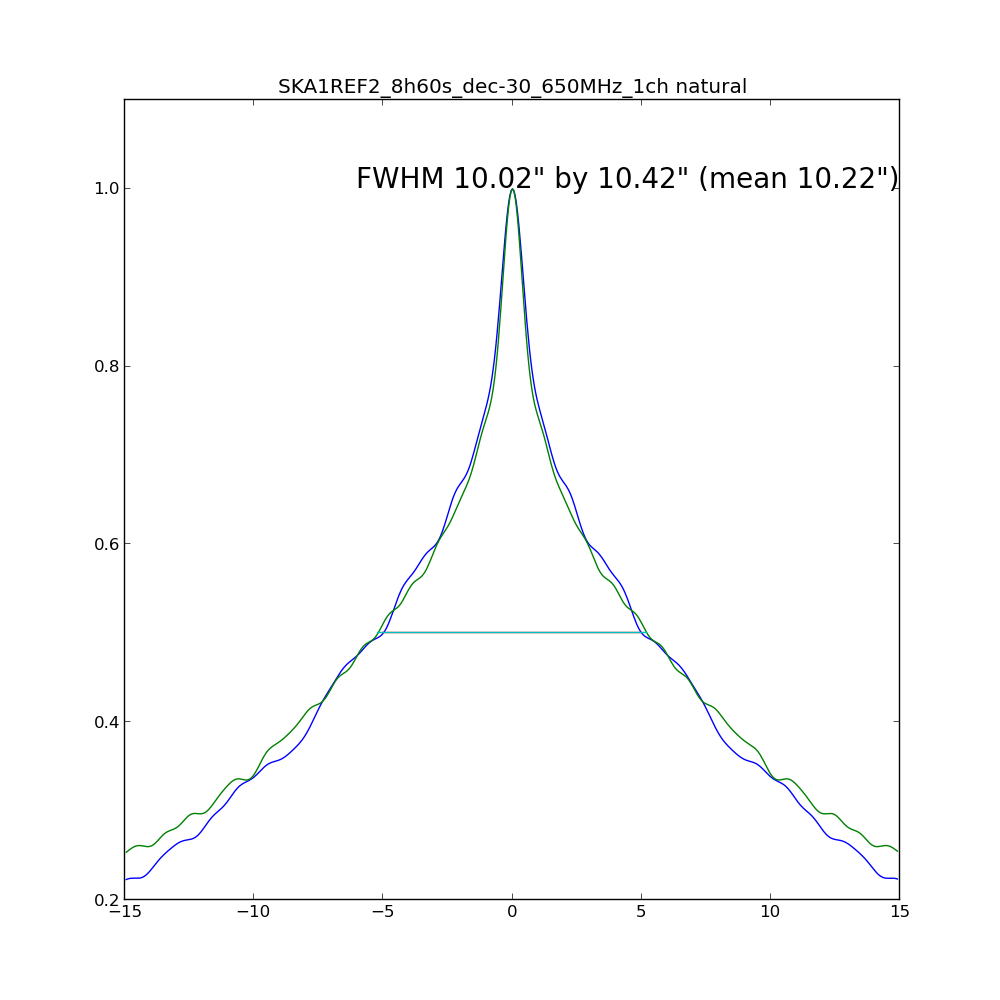
\includegraphics[width=0.180000\textwidth,trim= 0 .05cm 0 0.05cm]{{images/SKA1REF2_8h60s_dec-30_650MHz_1ch-natural-psf.fits}.png} &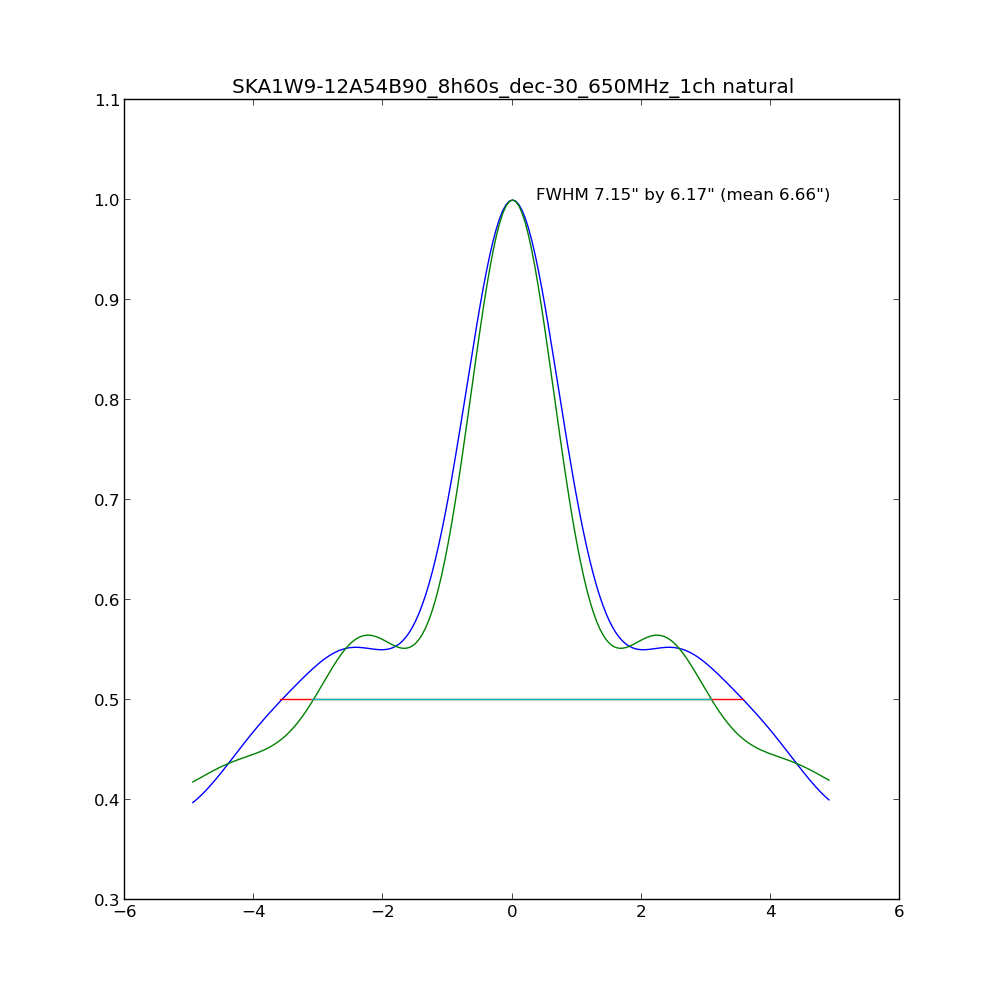
\includegraphics[width=0.180000\textwidth,trim= 0 .05cm 0 0.05cm]{{images/SKA1W9-12A54B90_8h60s_dec-30_650MHz_1ch-natural-psf.fits}.png} &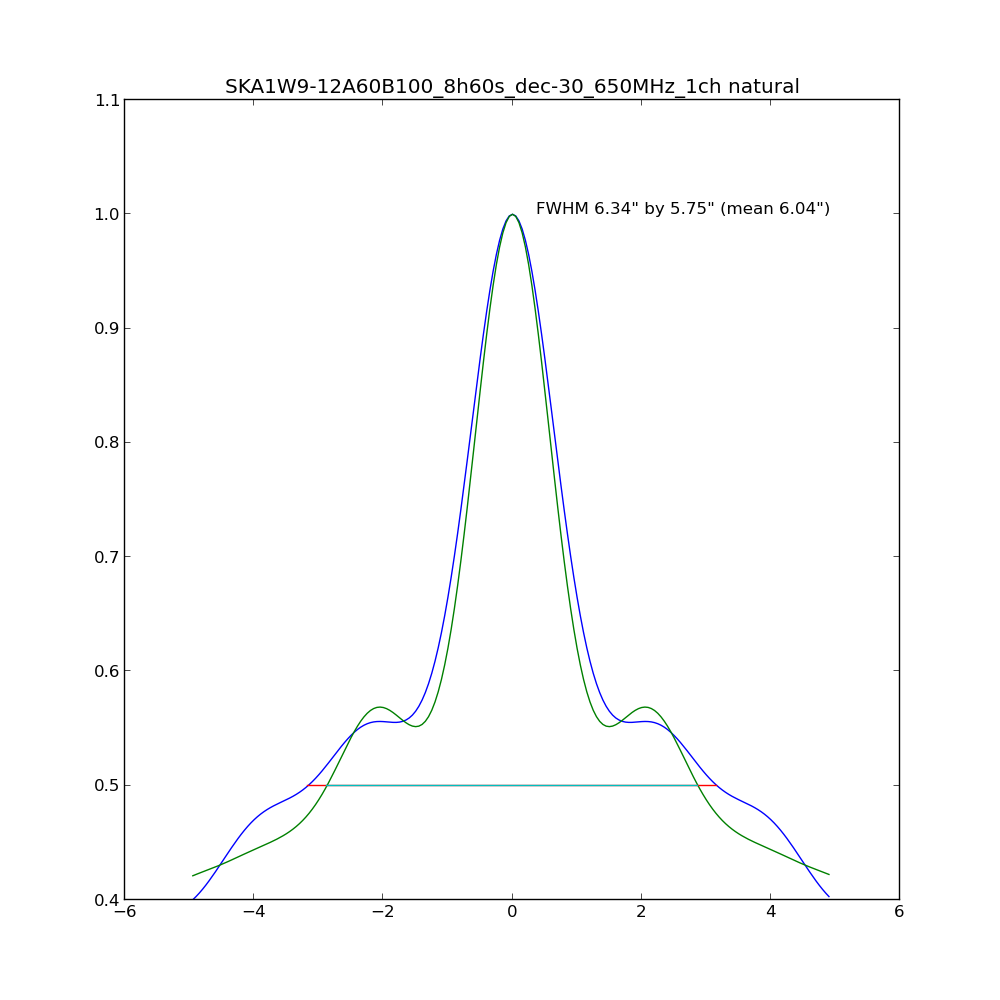
\includegraphics[width=0.180000\textwidth,trim= 0 .05cm 0 0.05cm]{{images/SKA1W9-12A60B100_8h60s_dec-30_650MHz_1ch-natural-psf.fits}.png} &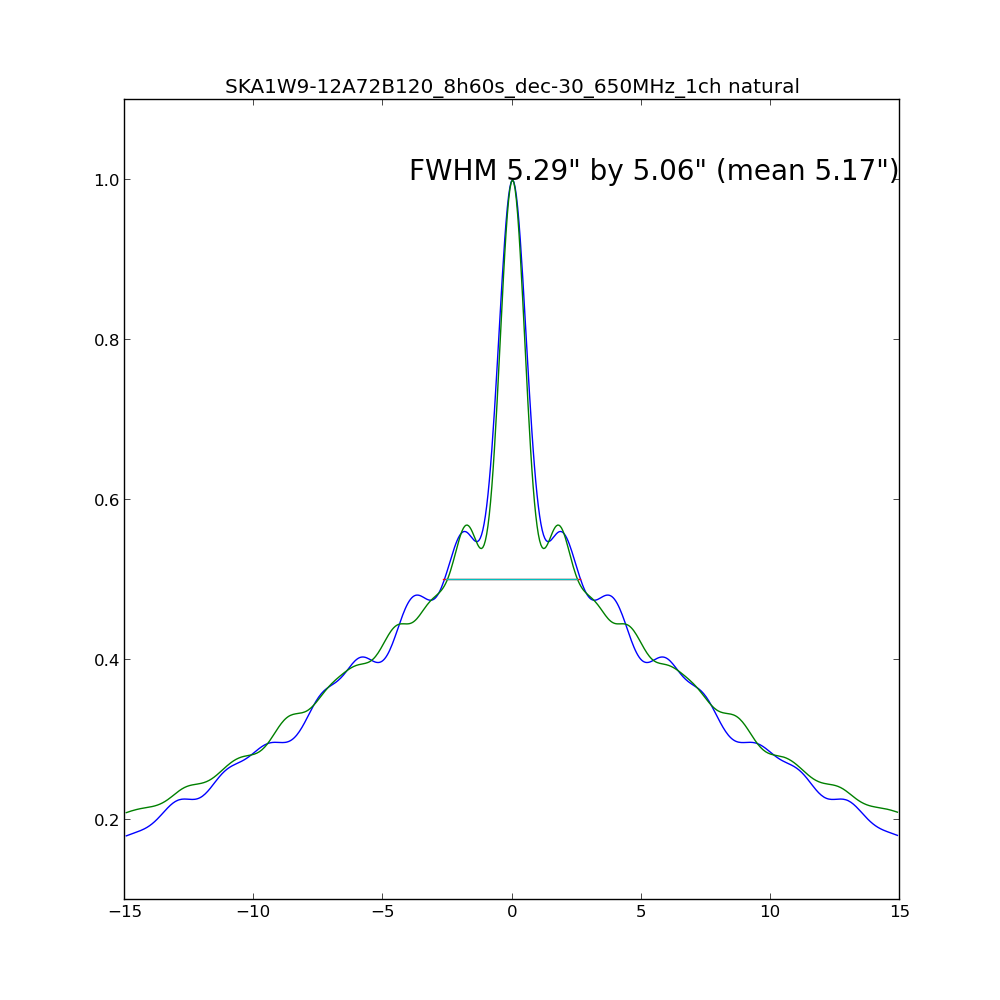
\includegraphics[width=0.180000\textwidth,trim= 0 .05cm 0 0.05cm]{{images/SKA1W9-12A72B120_8h60s_dec-30_650MHz_1ch-natural-psf.fits}.png} &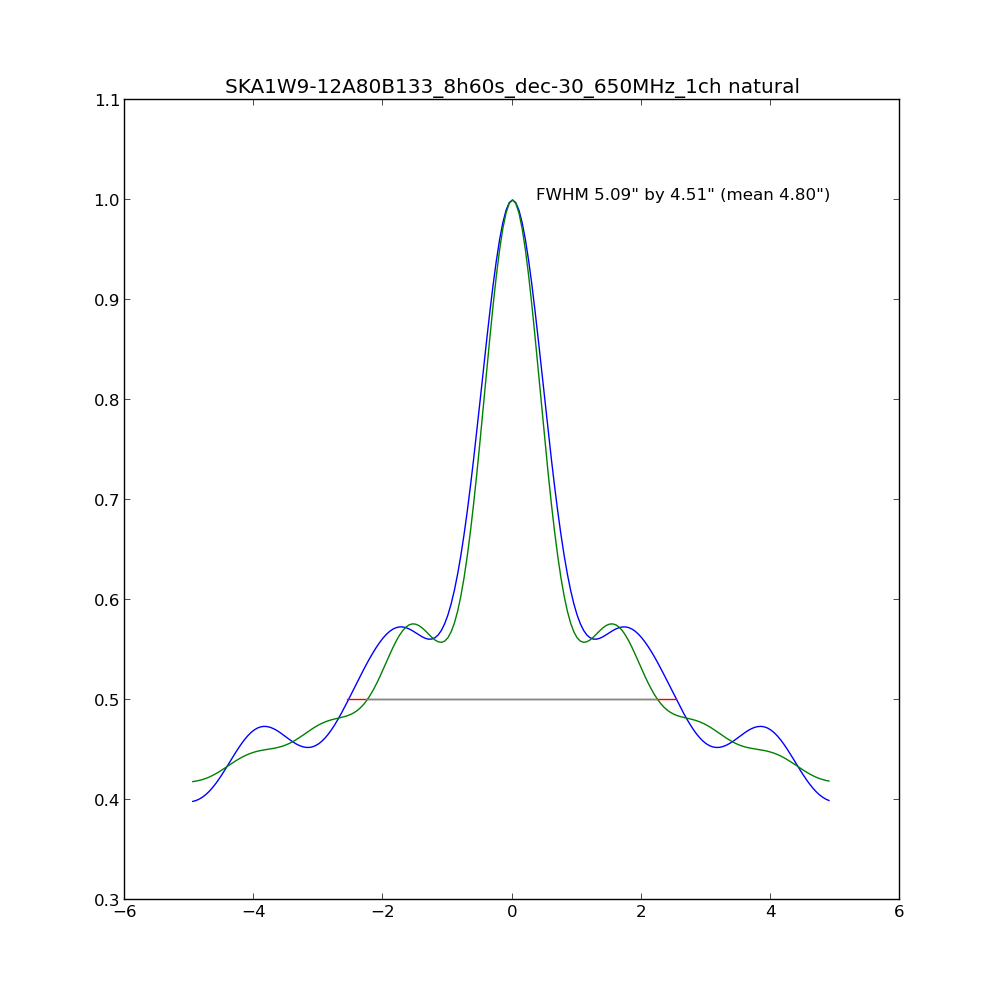
\includegraphics[width=0.180000\textwidth,trim= 0 .05cm 0 0.05cm]{{images/SKA1W9-12A80B133_8h60s_dec-30_650MHz_1ch-natural-psf.fits}.png} \\
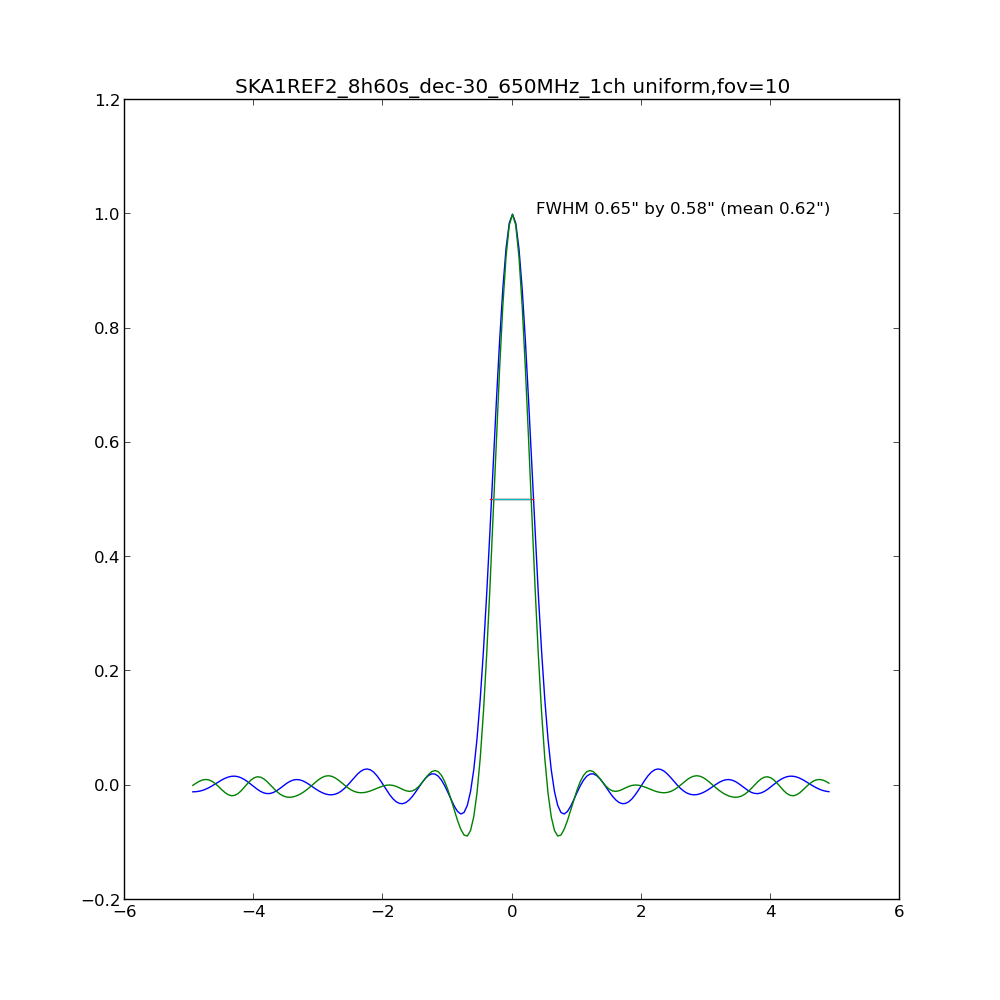
\includegraphics[width=0.180000\textwidth,trim= 0 .05cm 0 0.05cm]{{images/SKA1REF2_8h60s_dec-30_650MHz_1ch-uniform,fov=10-psf.fits}.png} &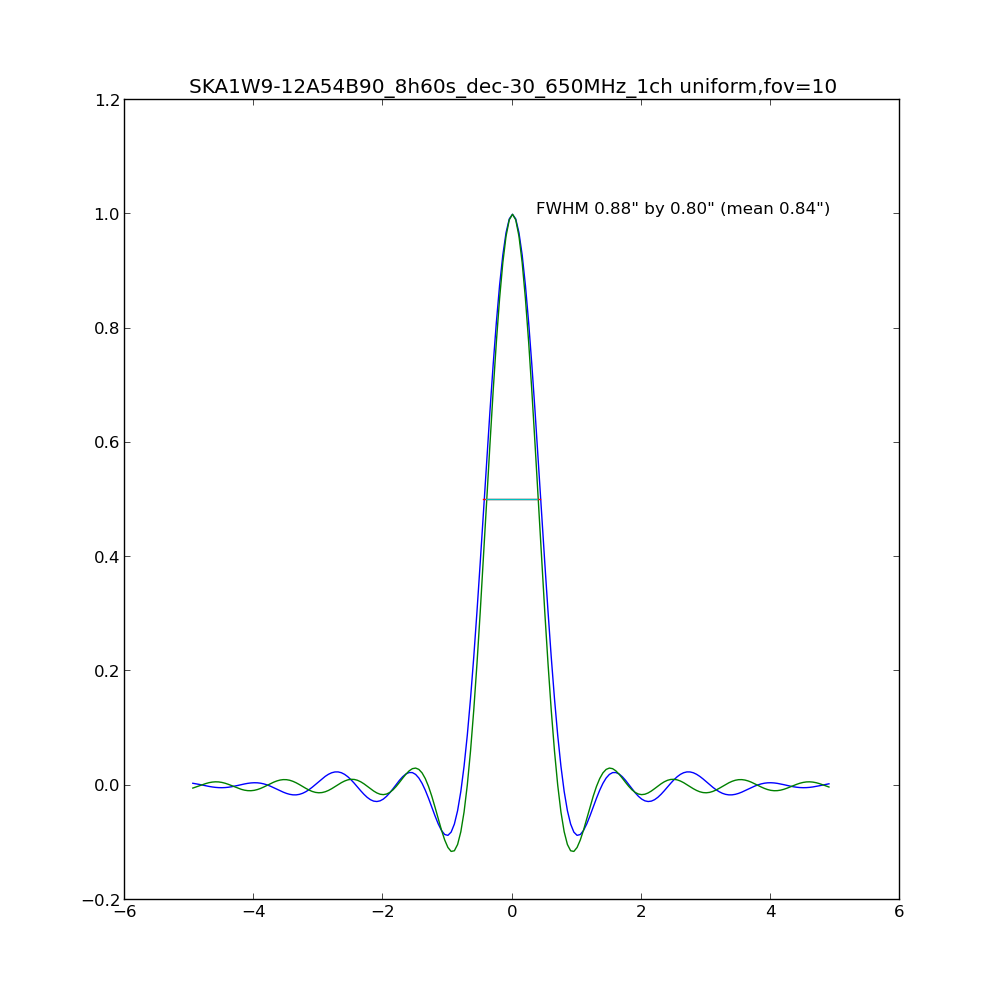
\includegraphics[width=0.180000\textwidth,trim= 0 .05cm 0 0.05cm]{{images/SKA1W9-12A54B90_8h60s_dec-30_650MHz_1ch-uniform,fov=10-psf.fits}.png} &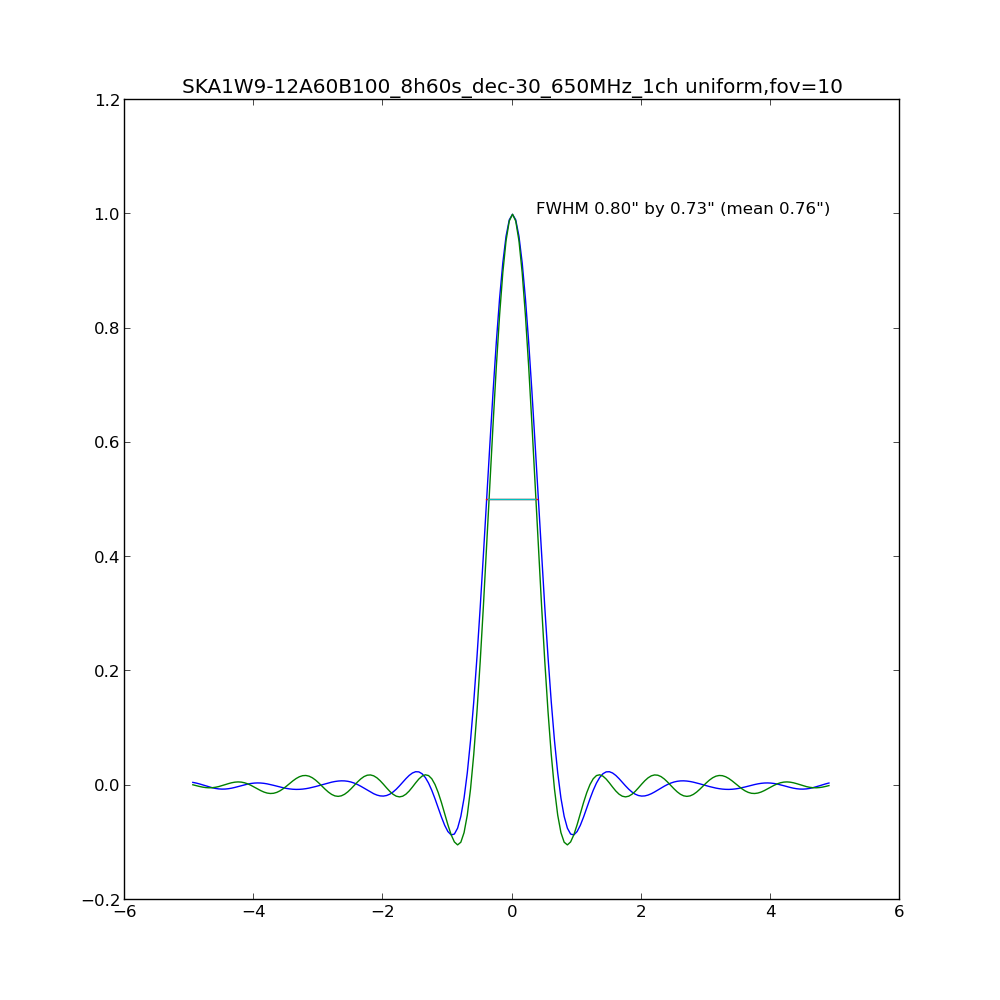
\includegraphics[width=0.180000\textwidth,trim= 0 .05cm 0 0.05cm]{{images/SKA1W9-12A60B100_8h60s_dec-30_650MHz_1ch-uniform,fov=10-psf.fits}.png} &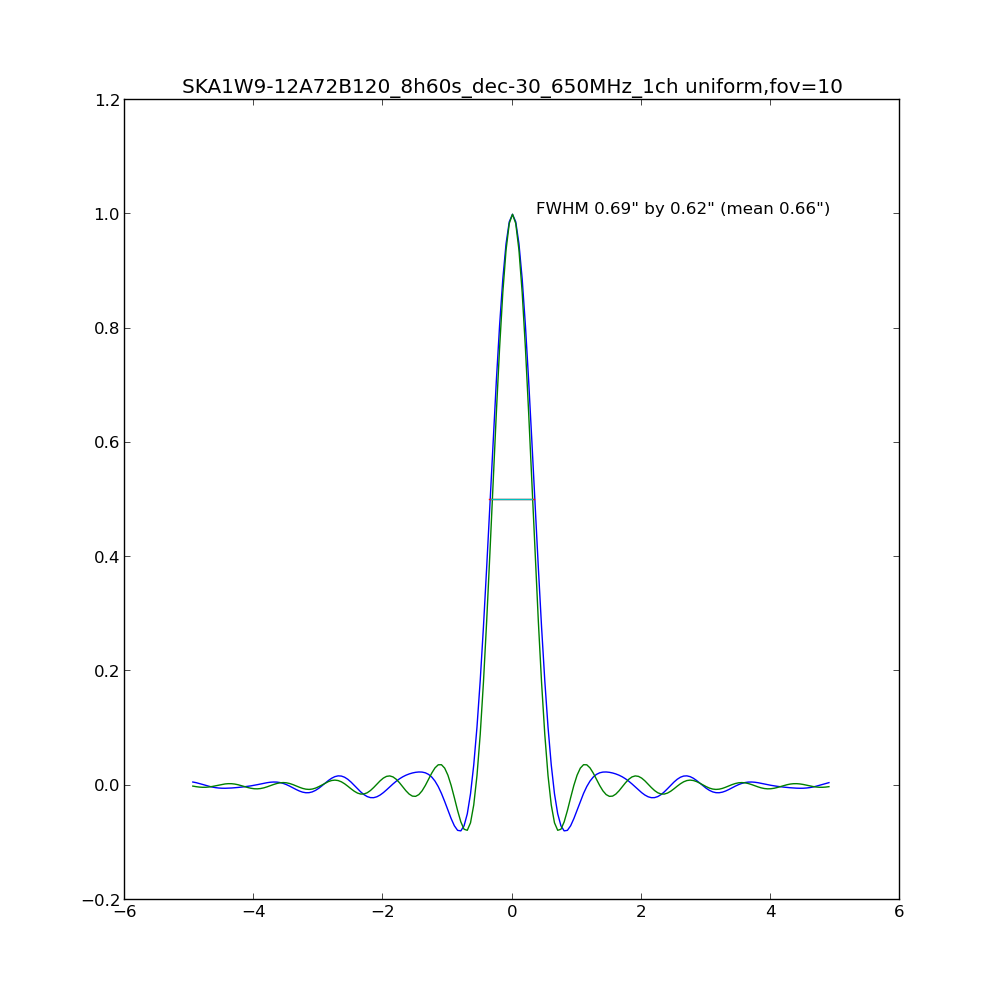
\includegraphics[width=0.180000\textwidth,trim= 0 .05cm 0 0.05cm]{{images/SKA1W9-12A72B120_8h60s_dec-30_650MHz_1ch-uniform,fov=10-psf.fits}.png} &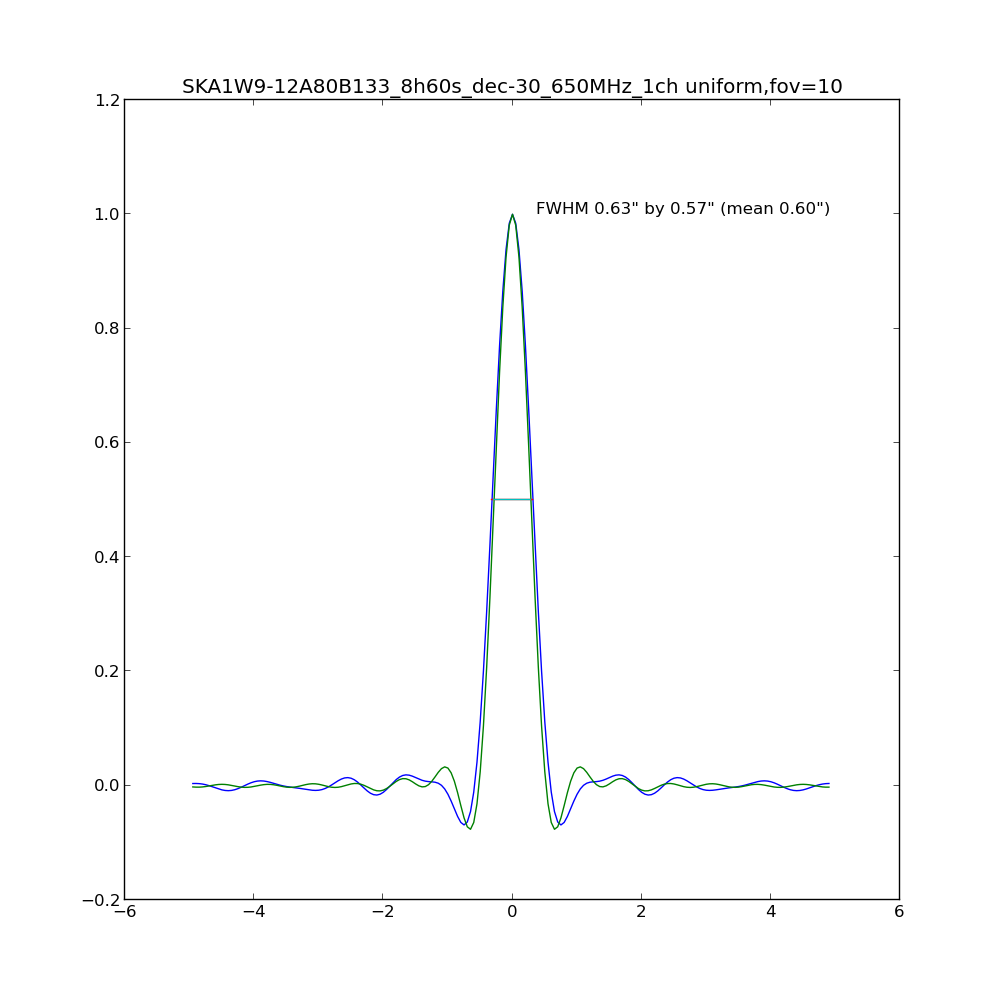
\includegraphics[width=0.180000\textwidth,trim= 0 .05cm 0 0.05cm]{{images/SKA1W9-12A80B133_8h60s_dec-30_650MHz_1ch-uniform,fov=10-psf.fits}.png} \\
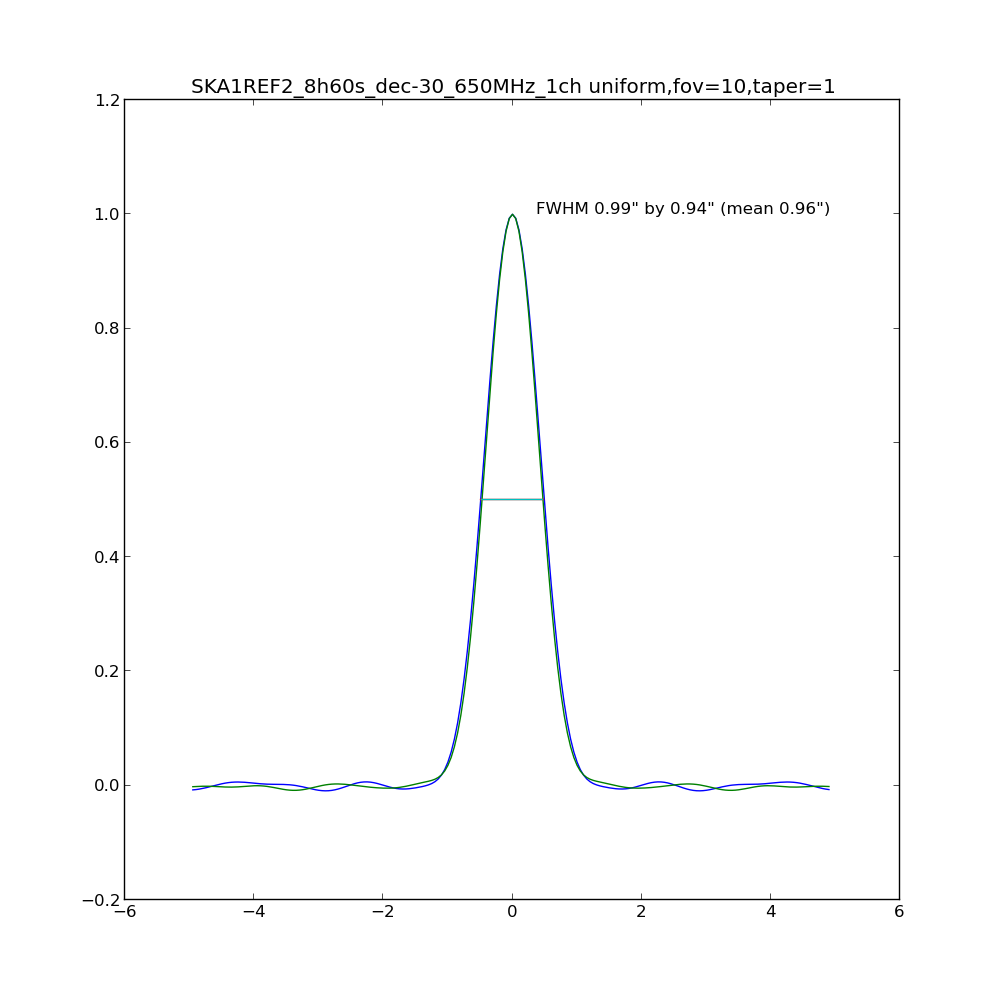
\includegraphics[width=0.180000\textwidth,trim= 0 .05cm 0 0.05cm]{{images/SKA1REF2_8h60s_dec-30_650MHz_1ch-uniform,fov=10,taper=1-psf.fits}.png} &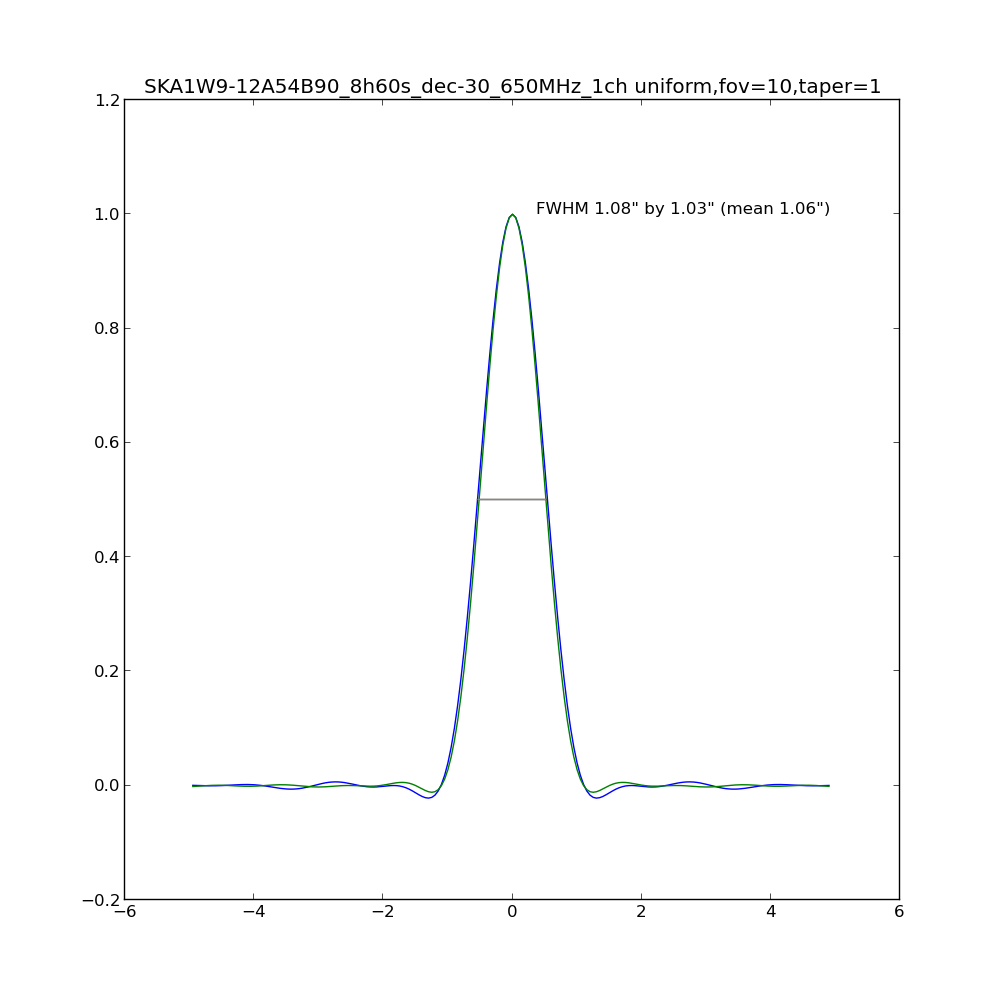
\includegraphics[width=0.180000\textwidth,trim= 0 .05cm 0 0.05cm]{{images/SKA1W9-12A54B90_8h60s_dec-30_650MHz_1ch-uniform,fov=10,taper=1-psf.fits}.png} &\includegraphics[width=0.180000\textwidth,trim= 0 .05cm 0 0.05cm]{{images/SKA1W9-12A60B100_8h60s_dec-30_650MHz_1ch-uniform,fov=10,taper=1-psf.fits}.png} &\includegraphics[width=0.180000\textwidth,trim= 0 .05cm 0 0.05cm]{{images/SKA1W9-12A72B120_8h60s_dec-30_650MHz_1ch-uniform,fov=10,taper=1-psf.fits}.png} &\includegraphics[width=0.180000\textwidth,trim= 0 .05cm 0 0.05cm]{{images/SKA1W9-12A80B133_8h60s_dec-30_650MHz_1ch-uniform,fov=10,taper=1-psf.fits}.png} 
\end{tabular}}
 \caption{PSF cross-sections at Dec=-30 deg, Freq=650MHz. Row 1 and 2 are for natural and uniform weighting respectively, and row
3 is for uniform weighting with a 1 arcsec Gaussian taper. The blue and green curves are cross-sections along $l$ and $m$
respectively, and the horizontal line marks the FWHM. FWHM parameters are included in the plot.}
\end{figure}
\begin{figure}[H]
 \tiny{%%% autogen
 \begin{tabular}{ccc}
\includegraphics[width=0.300000\textwidth,trim= 0 .05cm 0 0.05cm]{{images/SKA1REF2_8h60s_dec-30_800MHz_1ch-natural-psf.fits}.png} &\includegraphics[width=0.300000\textwidth,trim= 0 .05cm 0 0.05cm]{{images/SKA1W9-12A72B120_8h60s_dec-30_800MHz_1ch-natural-psf.fits}.png} &\includegraphics[width=0.300000\textwidth,trim= 0 .05cm 0 0.05cm]{{images/SKA1W9-0A72B120_8h60s_dec-30_800MHz_1ch-natural-psf.fits}.png} 
 \\\includegraphics[width=0.300000\textwidth,trim= 0 .05cm 0 0.05cm]{{images/SKA1REF2_8h60s_dec-30_800MHz_1ch-briggs,robust=-2,fov=10-psf.fits}.png} &\includegraphics[width=0.300000\textwidth,trim= 0 .05cm 0 0.05cm]{{images/SKA1W9-12A72B120_8h60s_dec-30_800MHz_1ch-briggs,robust=-2,fov=10-psf.fits}.png} &\includegraphics[width=0.300000\textwidth,trim= 0 .05cm 0 0.05cm]{{images/SKA1W9-0A72B120_8h60s_dec-30_800MHz_1ch-briggs,robust=-2,fov=10-psf.fits}.png} 
 \\\includegraphics[width=0.300000\textwidth,trim= 0 .05cm 0 0.05cm]{{images/SKA1REF2_8h60s_dec-30_800MHz_1ch-briggs,robust=-2,fov=10,taper=1-psf.fits}.png} &\includegraphics[width=0.300000\textwidth,trim= 0 .05cm 0 0.05cm]{{images/SKA1W9-12A72B120_8h60s_dec-30_800MHz_1ch-briggs,robust=-2,fov=10,taper=1-psf.fits}.png} &\includegraphics[width=0.300000\textwidth,trim= 0 .05cm 0 0.05cm]{{images/SKA1W9-0A72B120_8h60s_dec-30_800MHz_1ch-briggs,robust=-2,fov=10,taper=1-psf.fits}.png} 
 \\\end{tabular}}
 \caption{PSF cross-sections at Dec=-30 deg, Freq=800MHz. Row 1 and 2 are for natural and uniform weighting respectively, and  row
3 is for uniform weighting with a 1 arcsec Gaussian taper. The blue and green curves are cross-sections along $l$ and $m$
respectively, and the horizontal line marks the FWHM. FWHM parameters are included in the plot.}
\end{figure}
\begin{figure}[H]
 \tiny{%%% autogen
 \begin{tabular}{ccc}
\includegraphics[width=0.300000\textwidth,trim= 0 .05cm 0 0.05cm]{{images/SKA1REF2_8h60s_dec-30_1100MHz_1ch-natural-psf.fits}.png} &\includegraphics[width=0.300000\textwidth,trim= 0 .05cm 0 0.05cm]{{images/SKA1W9-12A72B120_8h60s_dec-30_1100MHz_1ch-natural-psf.fits}.png} &\includegraphics[width=0.300000\textwidth,trim= 0 .05cm 0 0.05cm]{{images/SKA1W9-0A72B120_8h60s_dec-30_1100MHz_1ch-natural-psf.fits}.png} 
 \\\includegraphics[width=0.300000\textwidth,trim= 0 .05cm 0 0.05cm]{{images/SKA1REF2_8h60s_dec-30_1100MHz_1ch-briggs,robust=-2,fov=10-psf.fits}.png} &\includegraphics[width=0.300000\textwidth,trim= 0 .05cm 0 0.05cm]{{images/SKA1W9-12A72B120_8h60s_dec-30_1100MHz_1ch-briggs,robust=-2,fov=10-psf.fits}.png} &\includegraphics[width=0.300000\textwidth,trim= 0 .05cm 0 0.05cm]{{images/SKA1W9-0A72B120_8h60s_dec-30_1100MHz_1ch-briggs,robust=-2,fov=10-psf.fits}.png} 
 \\\includegraphics[width=0.300000\textwidth,trim= 0 .05cm 0 0.05cm]{{images/SKA1REF2_8h60s_dec-30_1100MHz_1ch-briggs,robust=-2,fov=10,taper=1-psf.fits}.png} &\includegraphics[width=0.300000\textwidth,trim= 0 .05cm 0 0.05cm]{{images/SKA1W9-12A72B120_8h60s_dec-30_1100MHz_1ch-briggs,robust=-2,fov=10,taper=1-psf.fits}.png} &\includegraphics[width=0.300000\textwidth,trim= 0 .05cm 0 0.05cm]{{images/SKA1W9-0A72B120_8h60s_dec-30_1100MHz_1ch-briggs,robust=-2,fov=10,taper=1-psf.fits}.png} 
 \\\end{tabular}}
 \caption{PSF cross-sections at Dec=-30 deg, Freq=1100MHz. Row 1 and 2 are for natural and uniform weighting respectively, and row
3 is for uniform weighting with a 1 arcsec Gaussian taper. The blue and green curves are cross-sections along $l$ and $m$
respectively, and the horizontal line marks the FWHM. FWHM parameters are included in the plot.}
\end{figure}

\end{document}

